%!TEX root = ../Report.tex

% User Manual
\chapter{User's Manual} % (fold)
\label{cha:user_s_manual}

\section{Prerequisite} % (fold)
\label{sec:prerequisite}
To use Dialogflow and Slack, the following account is required:
\begin{itemize}
	\item Gmail Account
	\item Slack Account
\end{itemize}
If you do not have these two accounts, please go to Slack (https://slack.com/signin) or Google (https://accounts.google.com/sigNup) to register.

\clearpage
% section prerequisite (end)


\section{Import Agent} % (fold)
\label{sec:import_agent}

\begin{enumerate}

	\item Go to Dialogflow Console (https://console.dialogflow.com), then click “Create new agent”

	\begin{figure}[H]
		\centering
		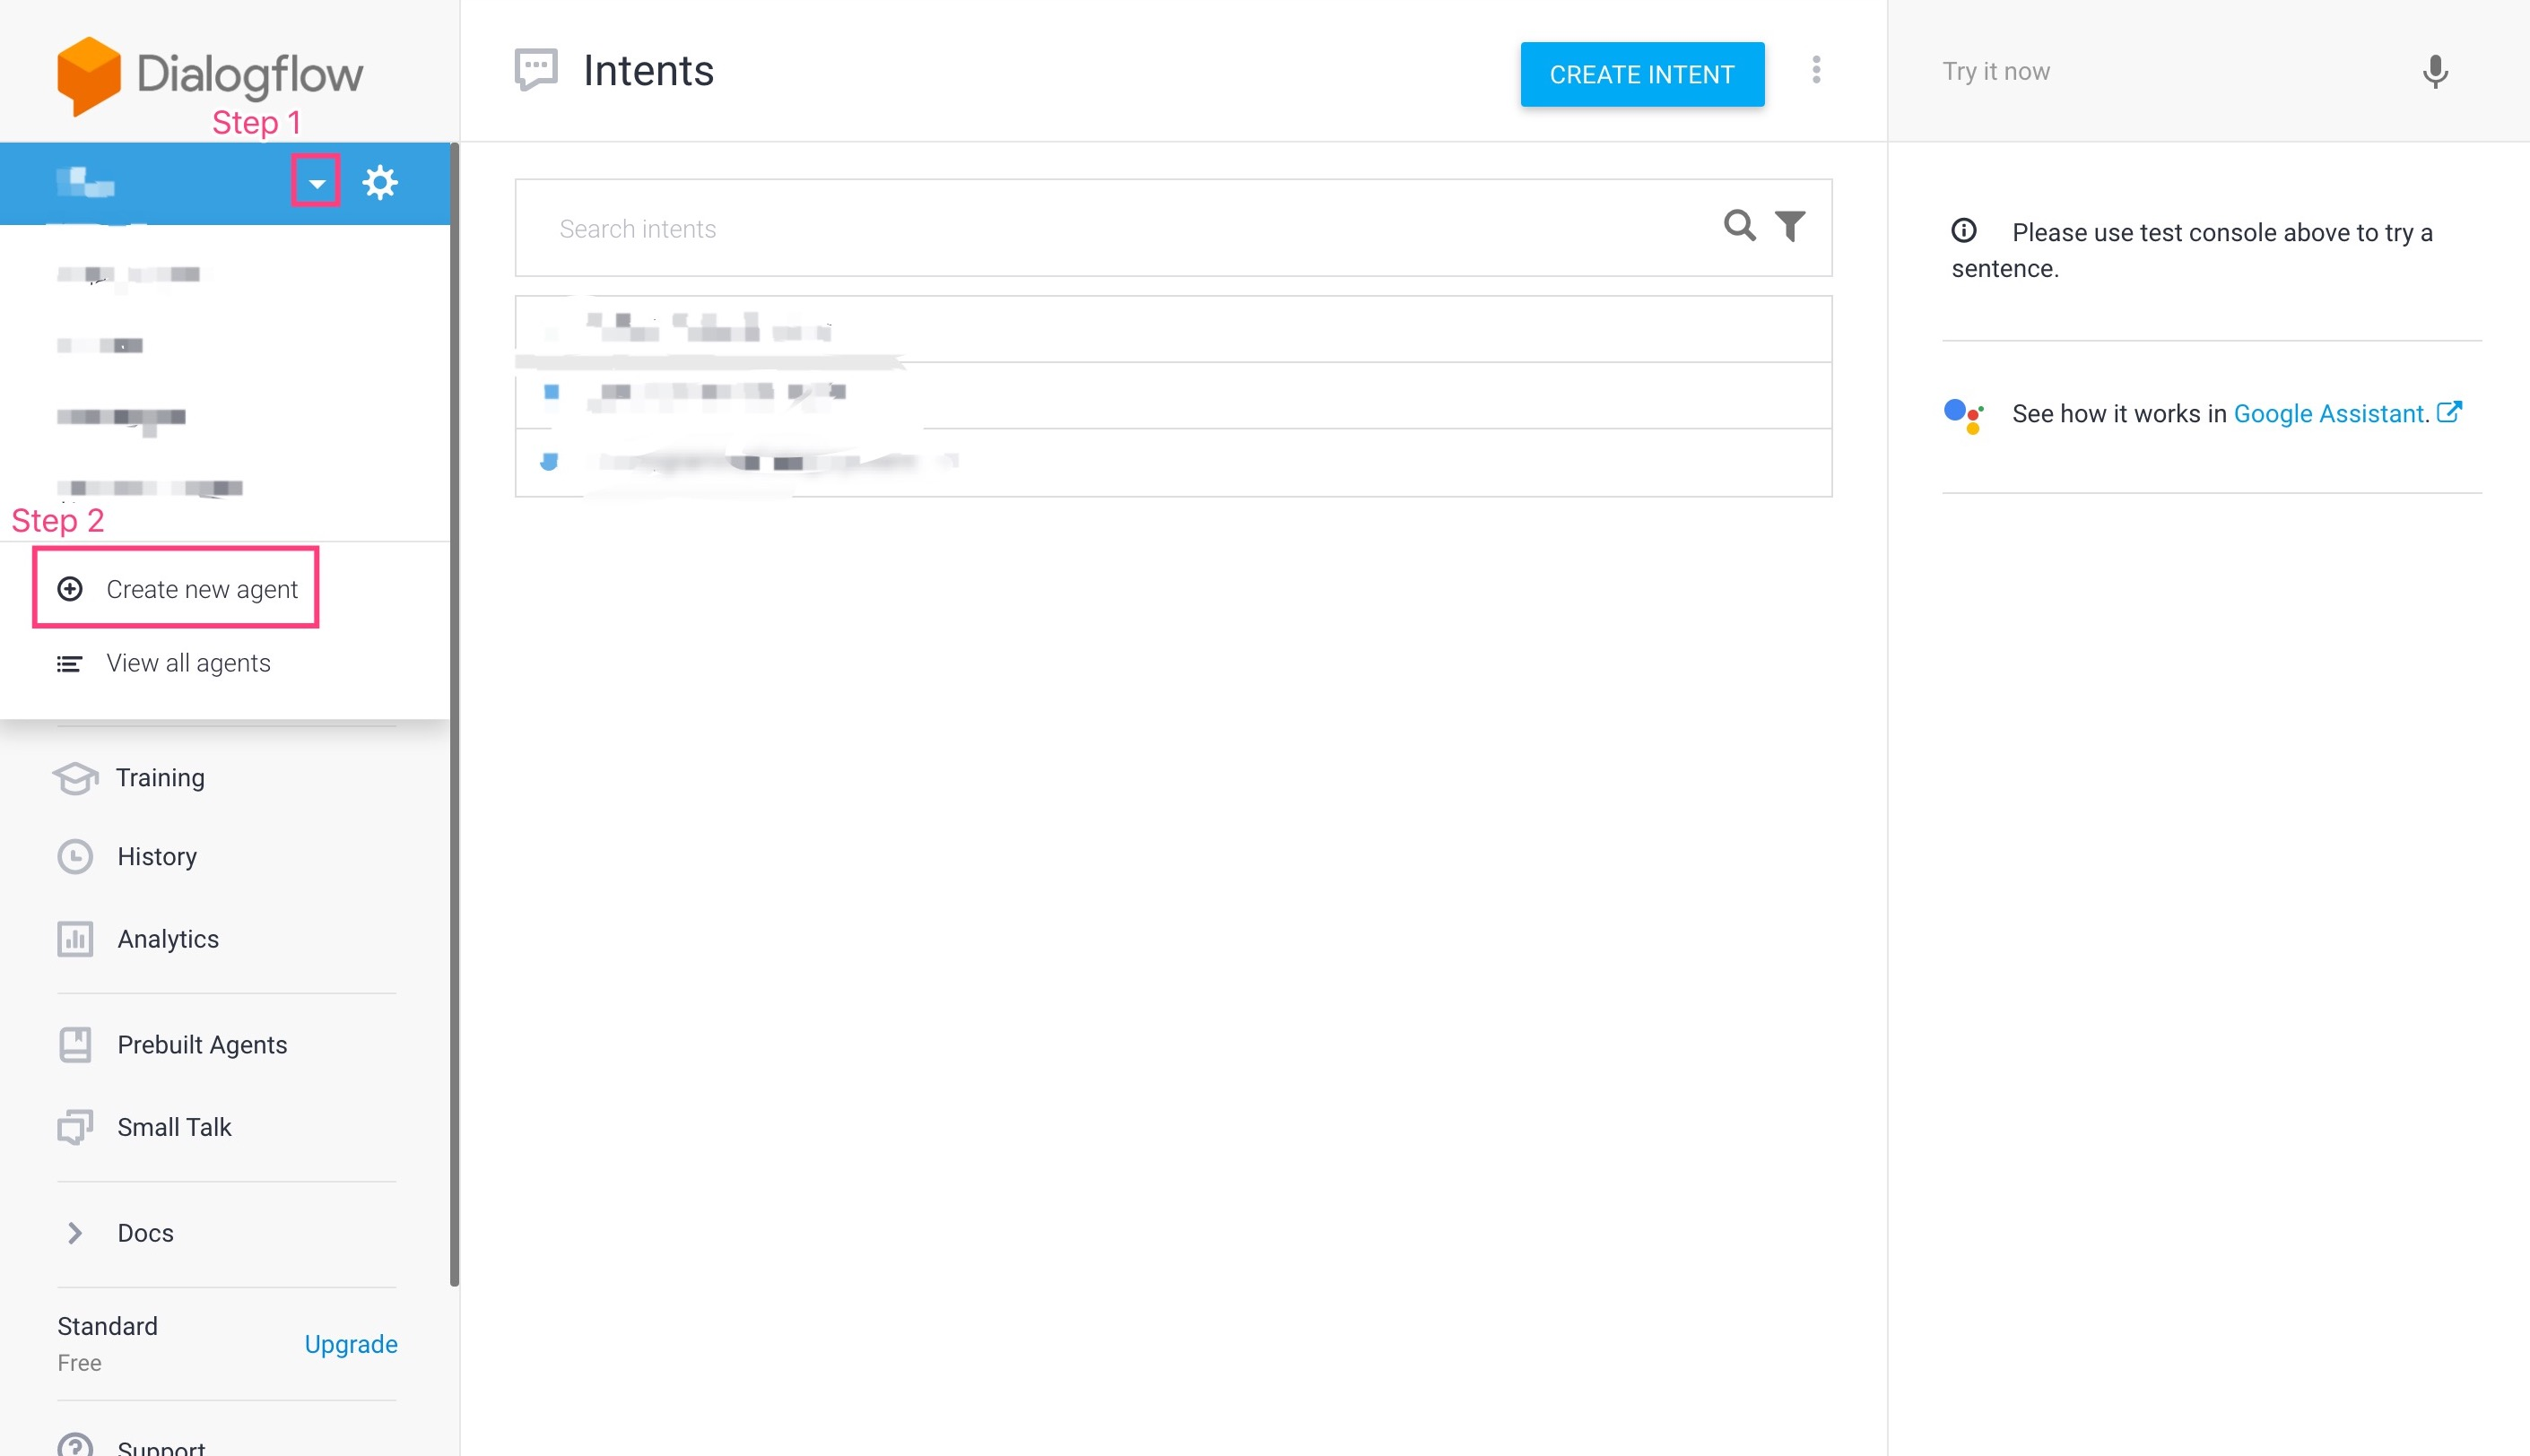
\includegraphics[width=\linewidth, frame]{img/manual_1.jpg}
	\end{figure}

	\item Put Agent name as you wish, then click “CREATE” button

	\begin{figure}[H]
		\centering
		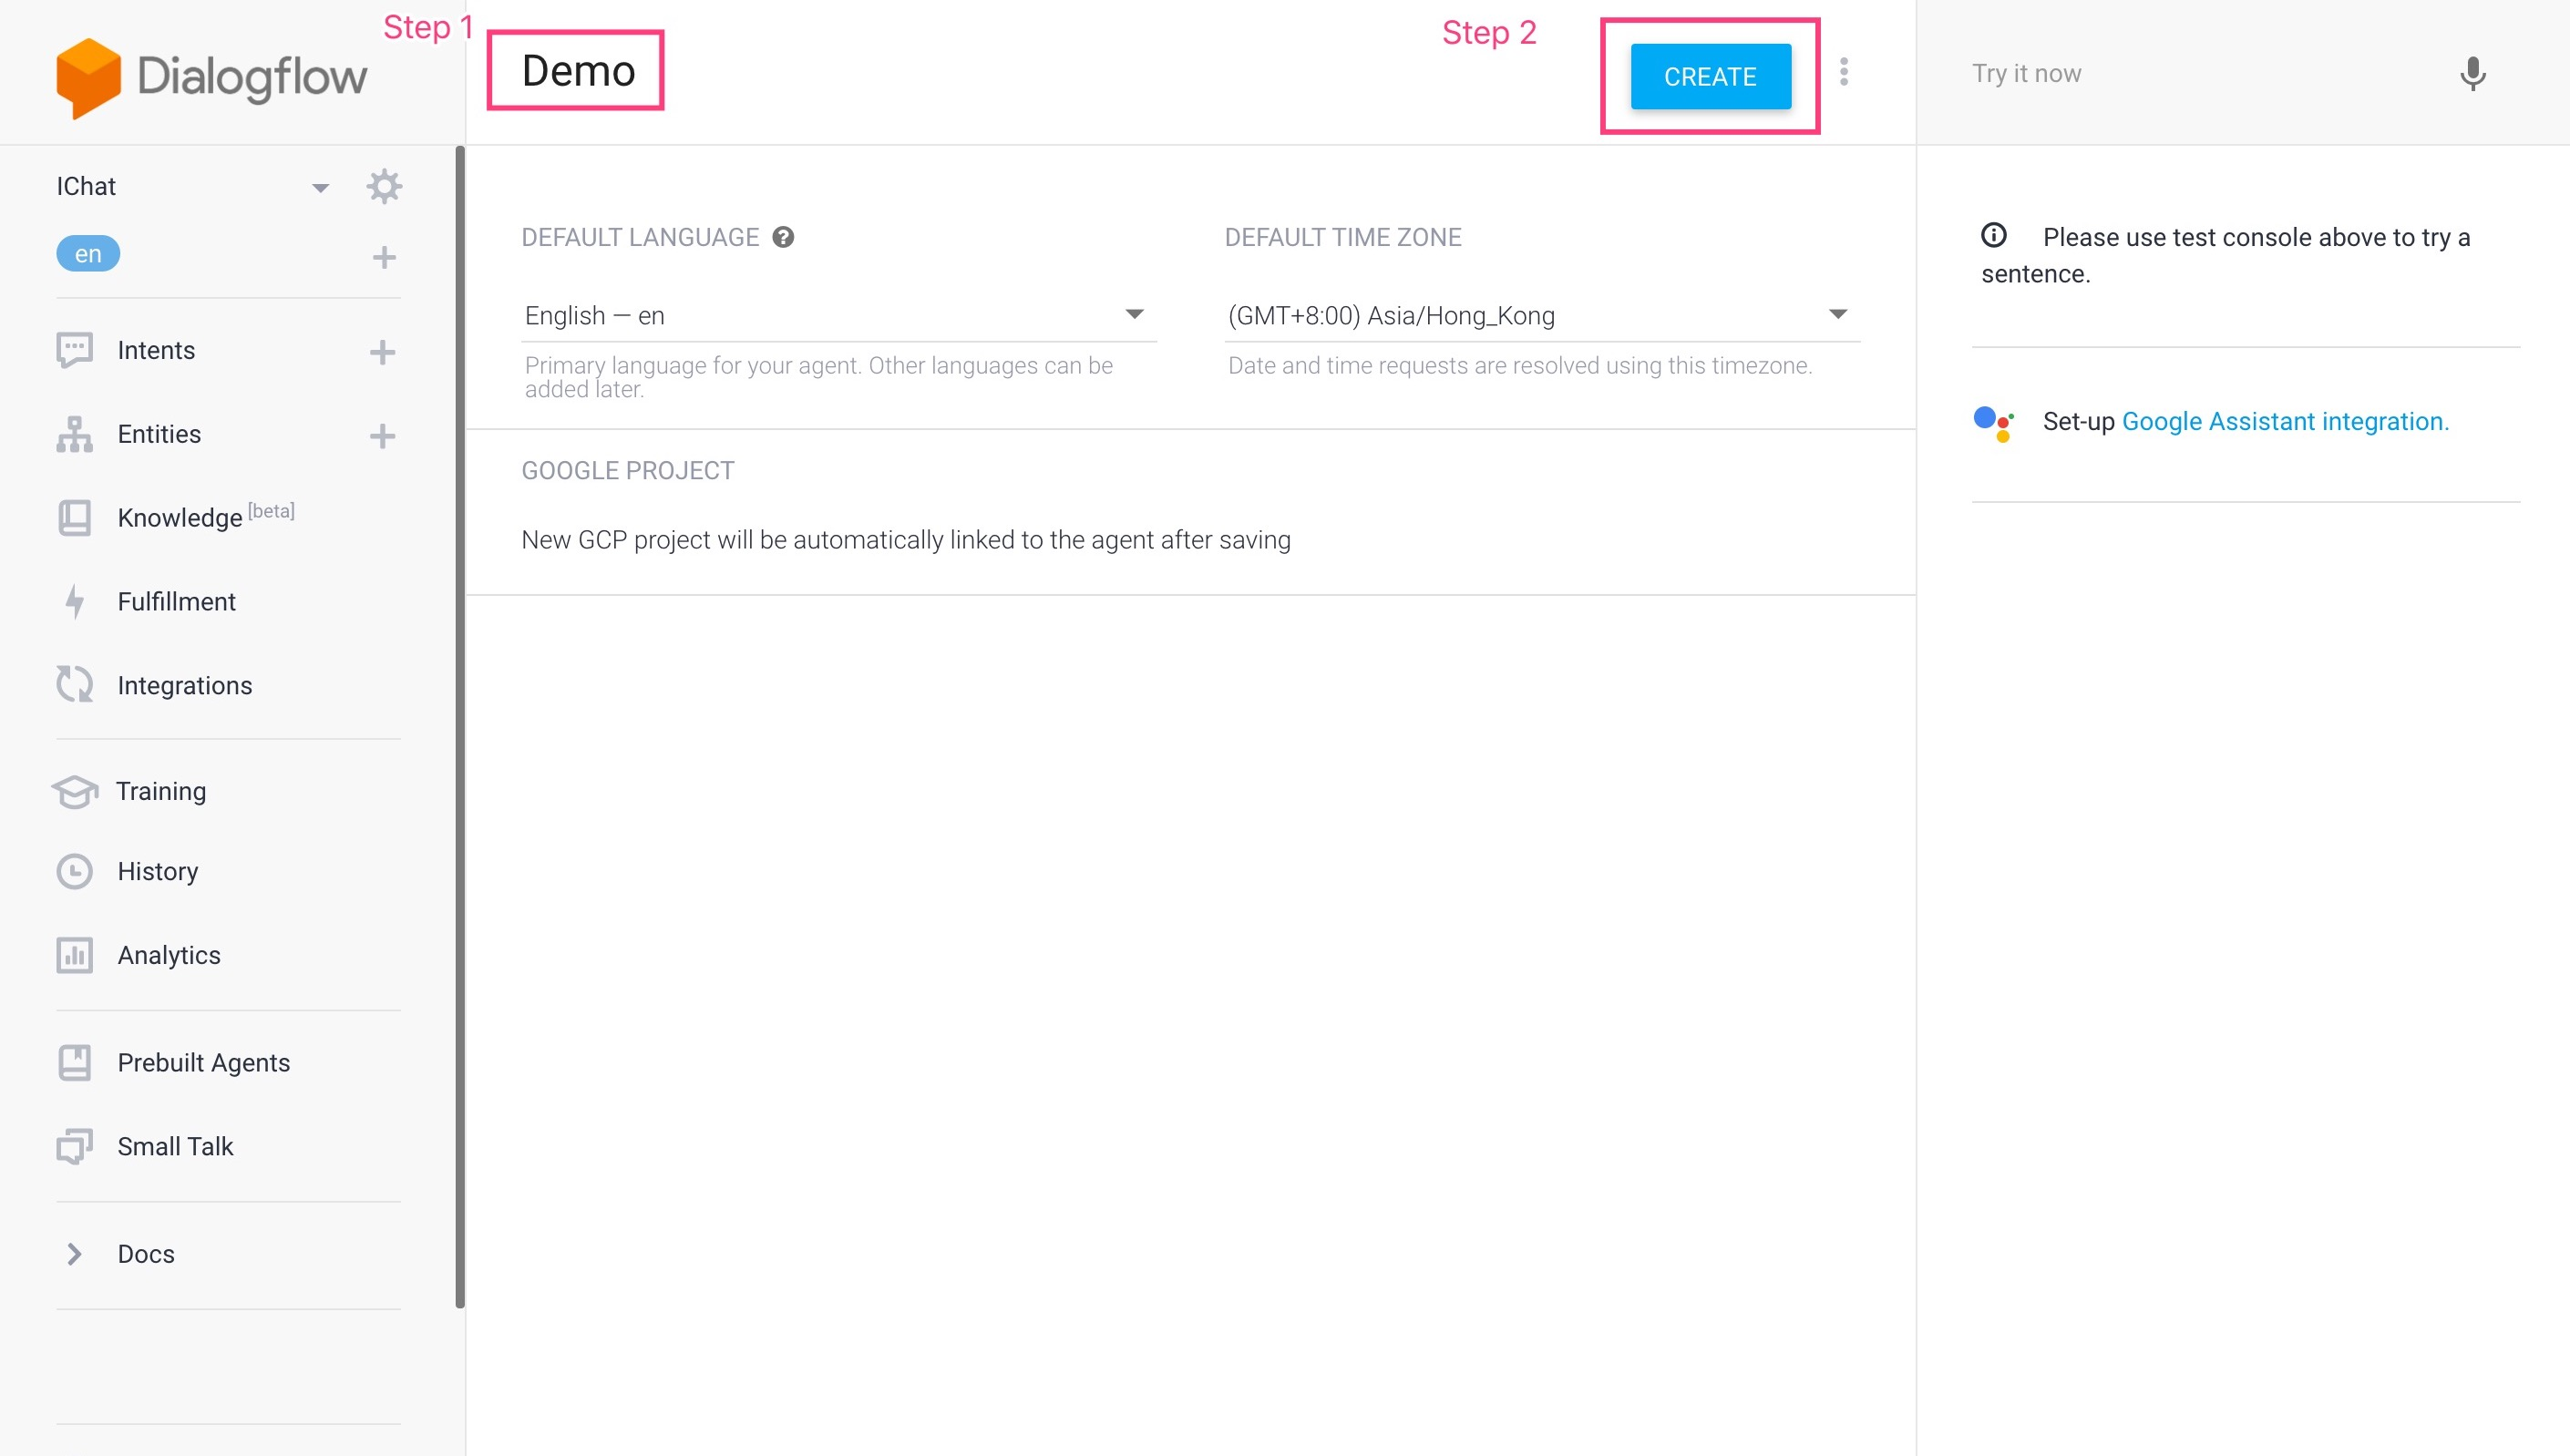
\includegraphics[width=\linewidth, frame]{img/manual_2.jpg}
	\end{figure}

	\item Go to Settings and enable beta features and APIs
	\nopagebreak
	\begin{figure}[H]
		\centering
		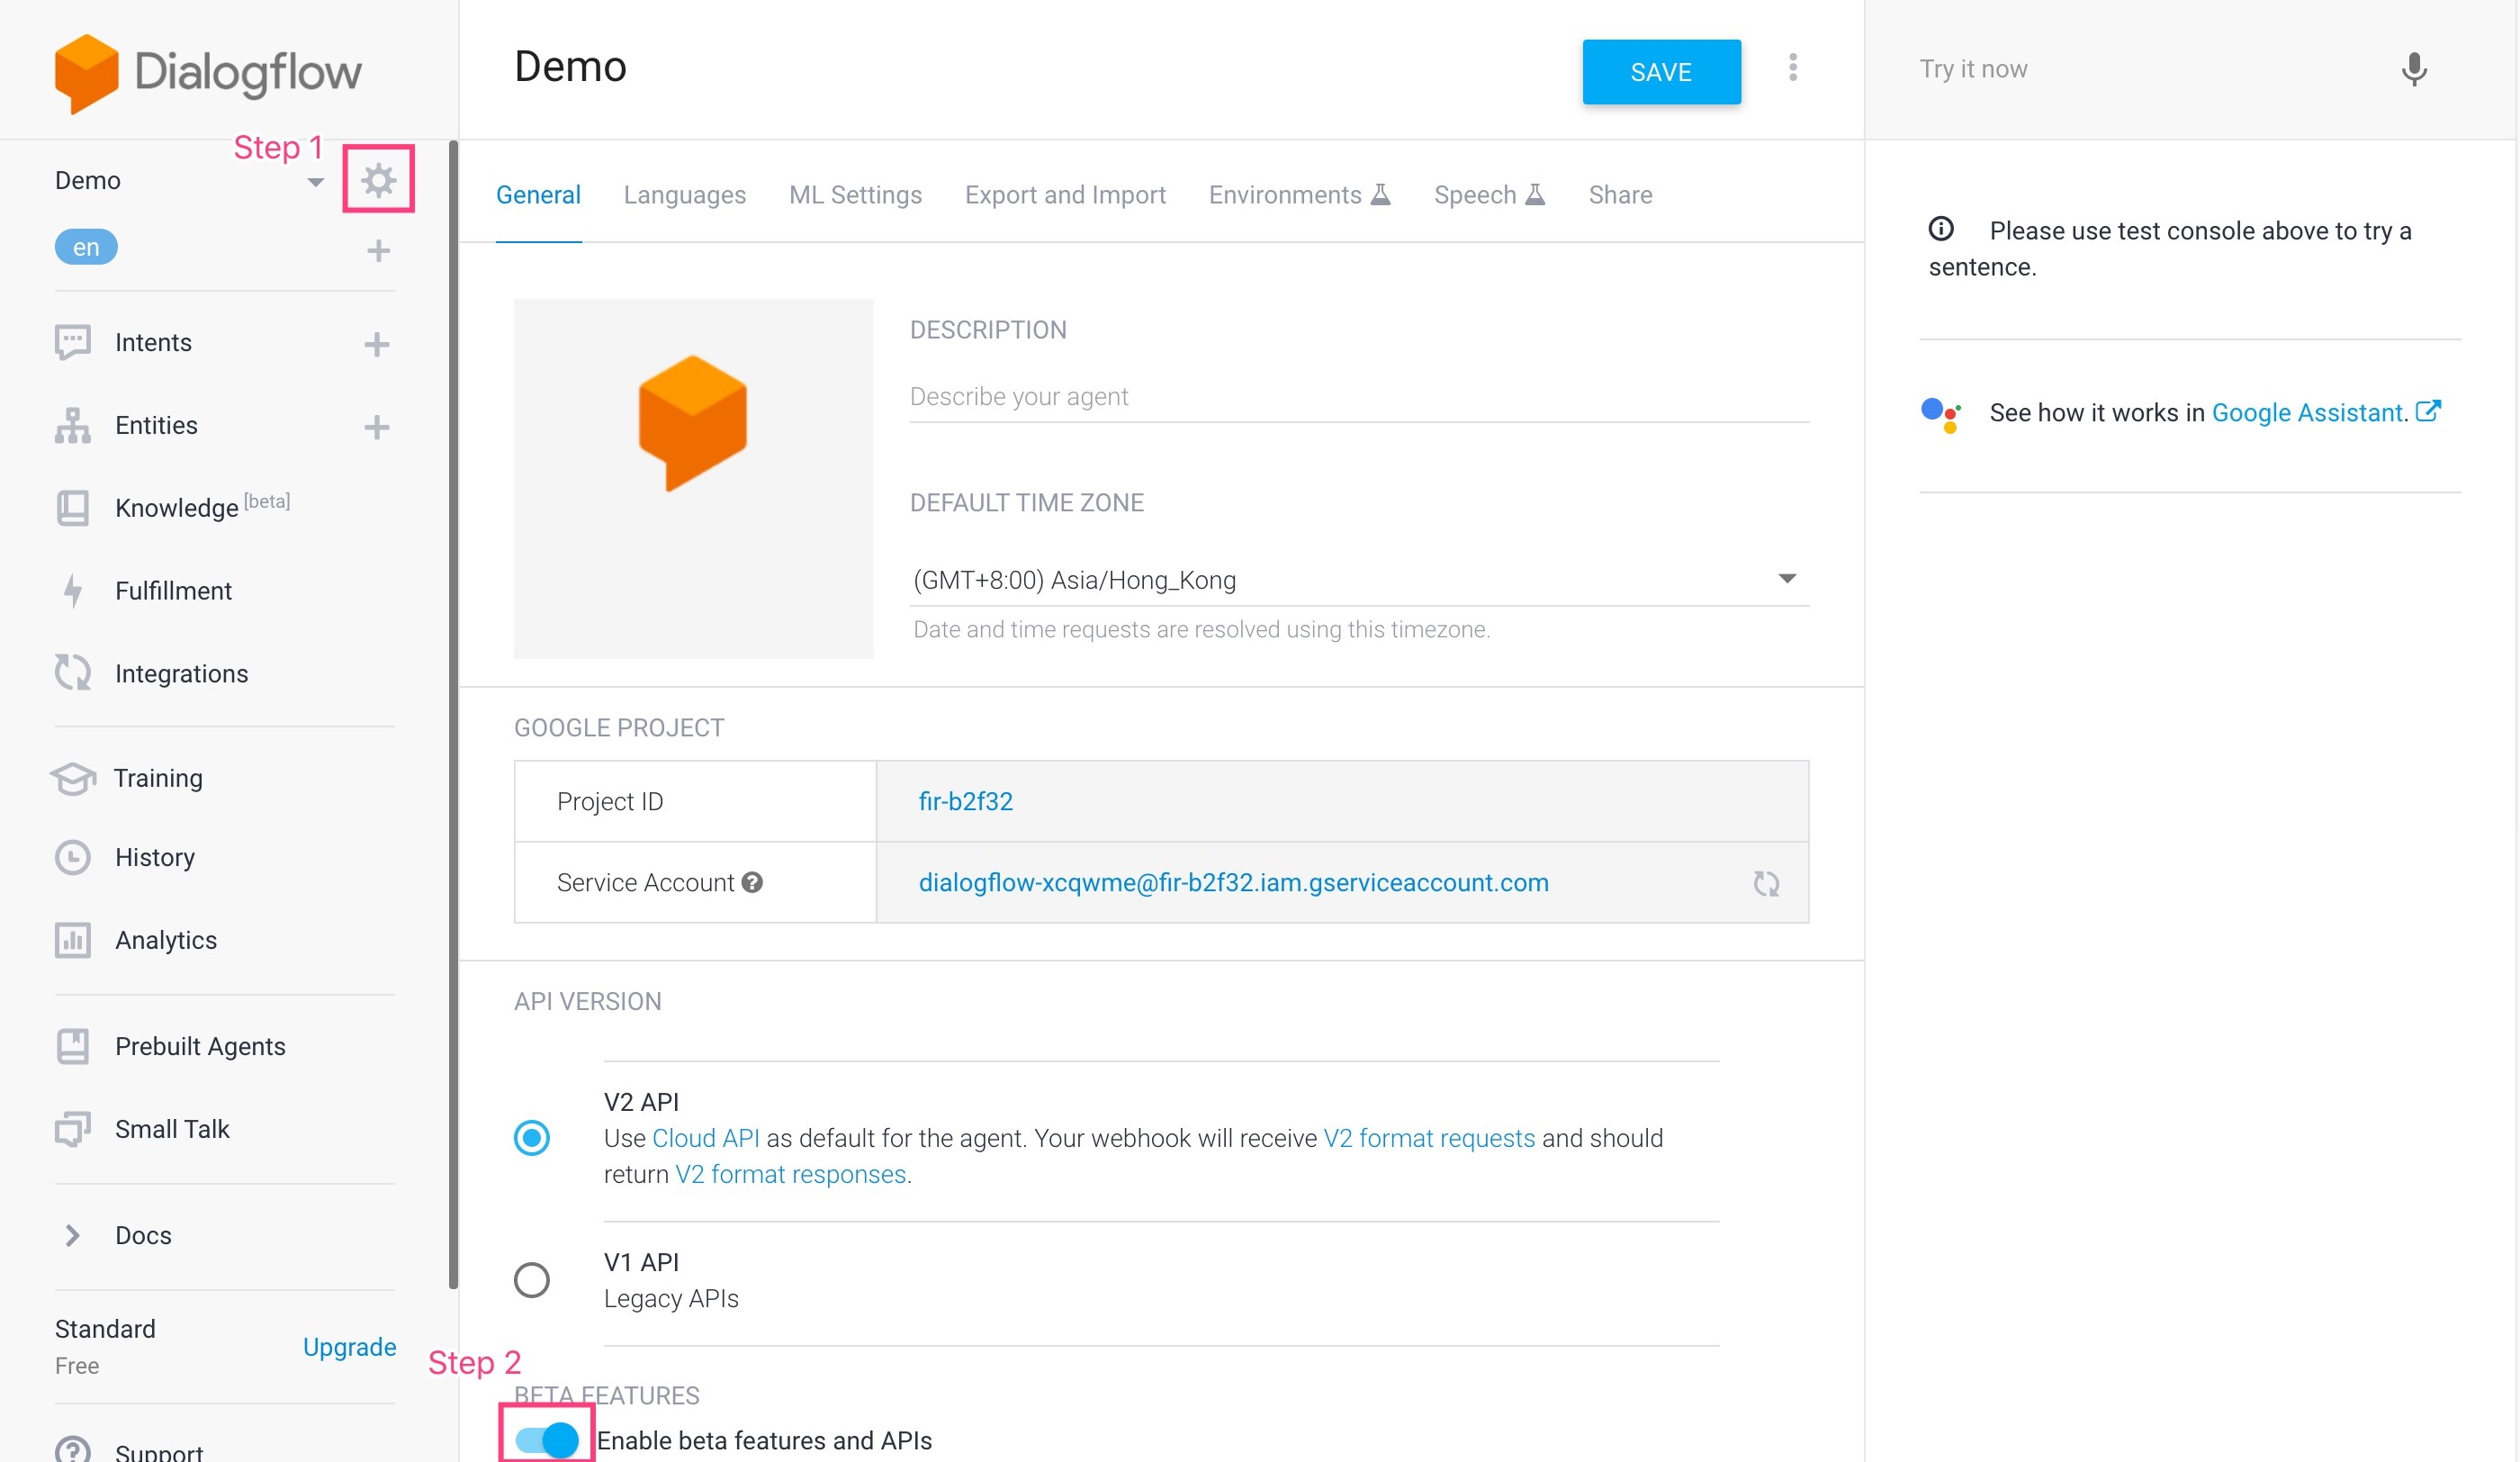
\includegraphics[width=\linewidth, frame]{img/manual_3.jpg}
	\end{figure}

	\item Go to “Export and Import” and click “IMPORT FROM ZIP”

	\begin{figure}[H]
		\centering
		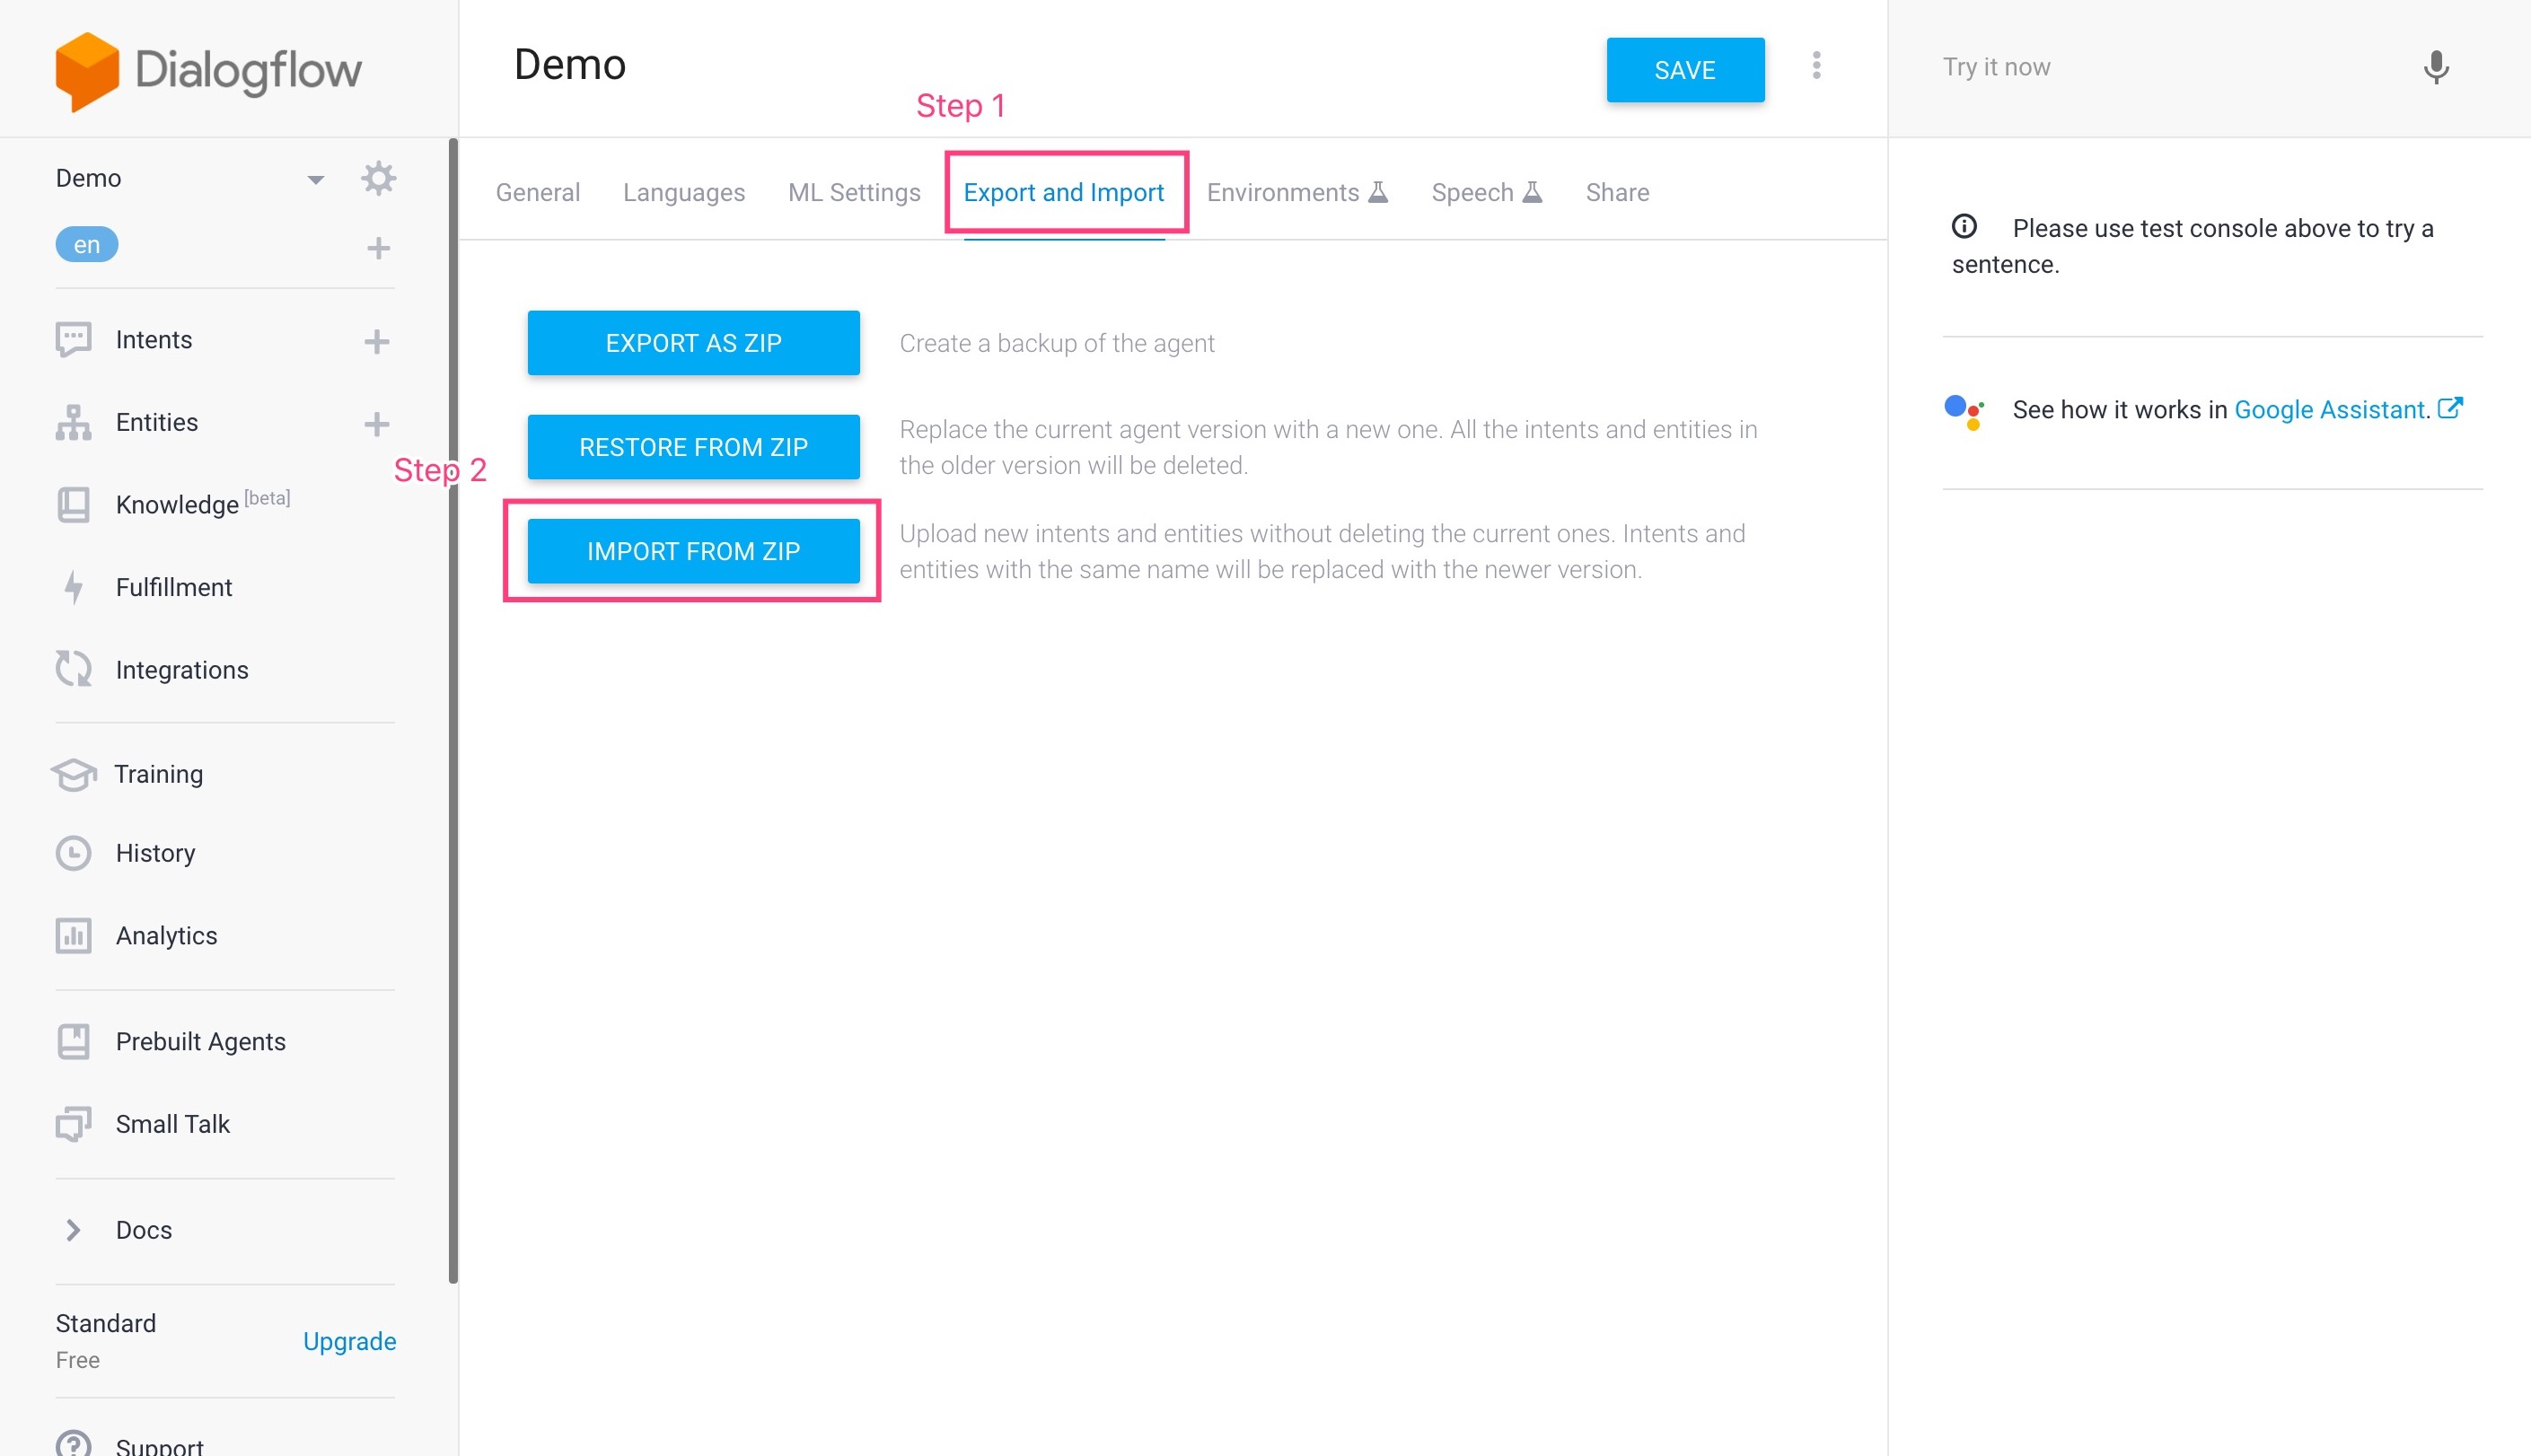
\includegraphics[width=\linewidth, frame]{img/manual_4.jpg}
	\end{figure}

	\item Click “SELECT FILE”
	\nopagebreak
	\begin{figure}[H]
		\centering
		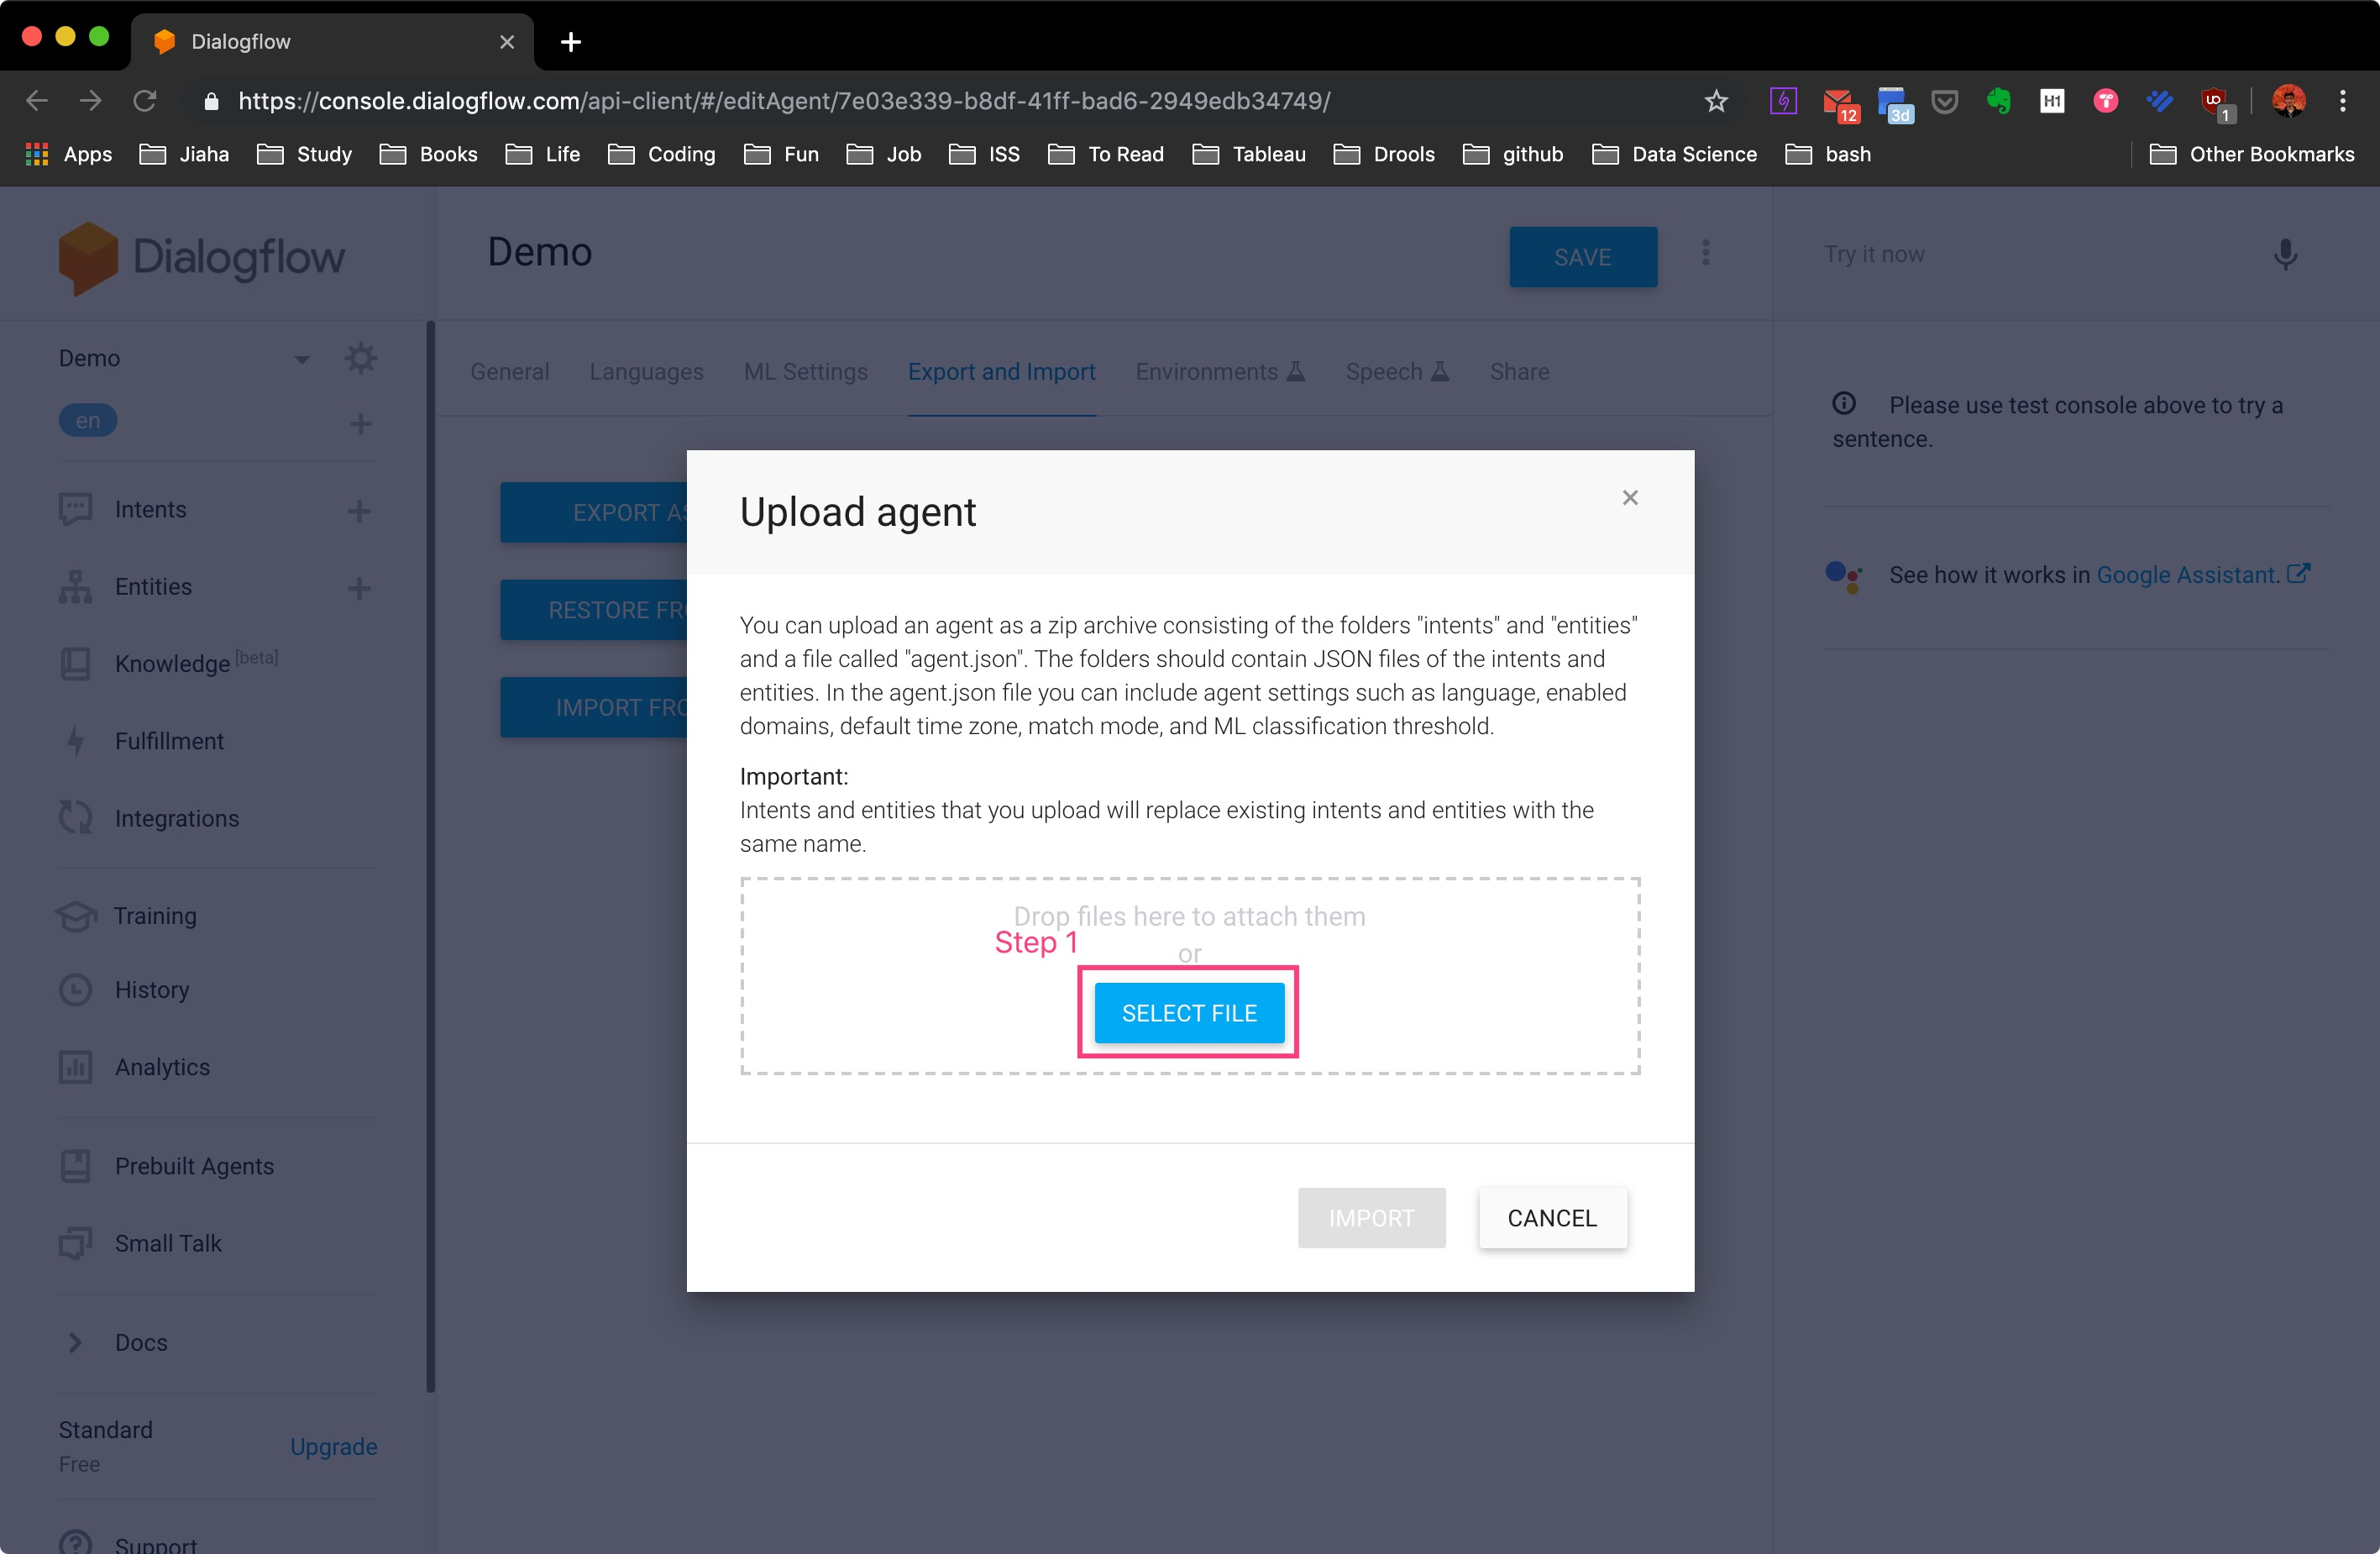
\includegraphics[width=\linewidth, frame]{img/manual_5.jpg}
	\end{figure}

	\item Choose “IChat.zip”, type IMPORT and click “IMPORT” button. Click “Done” button once imported.

	\begin{figure}[H]
		\centering
		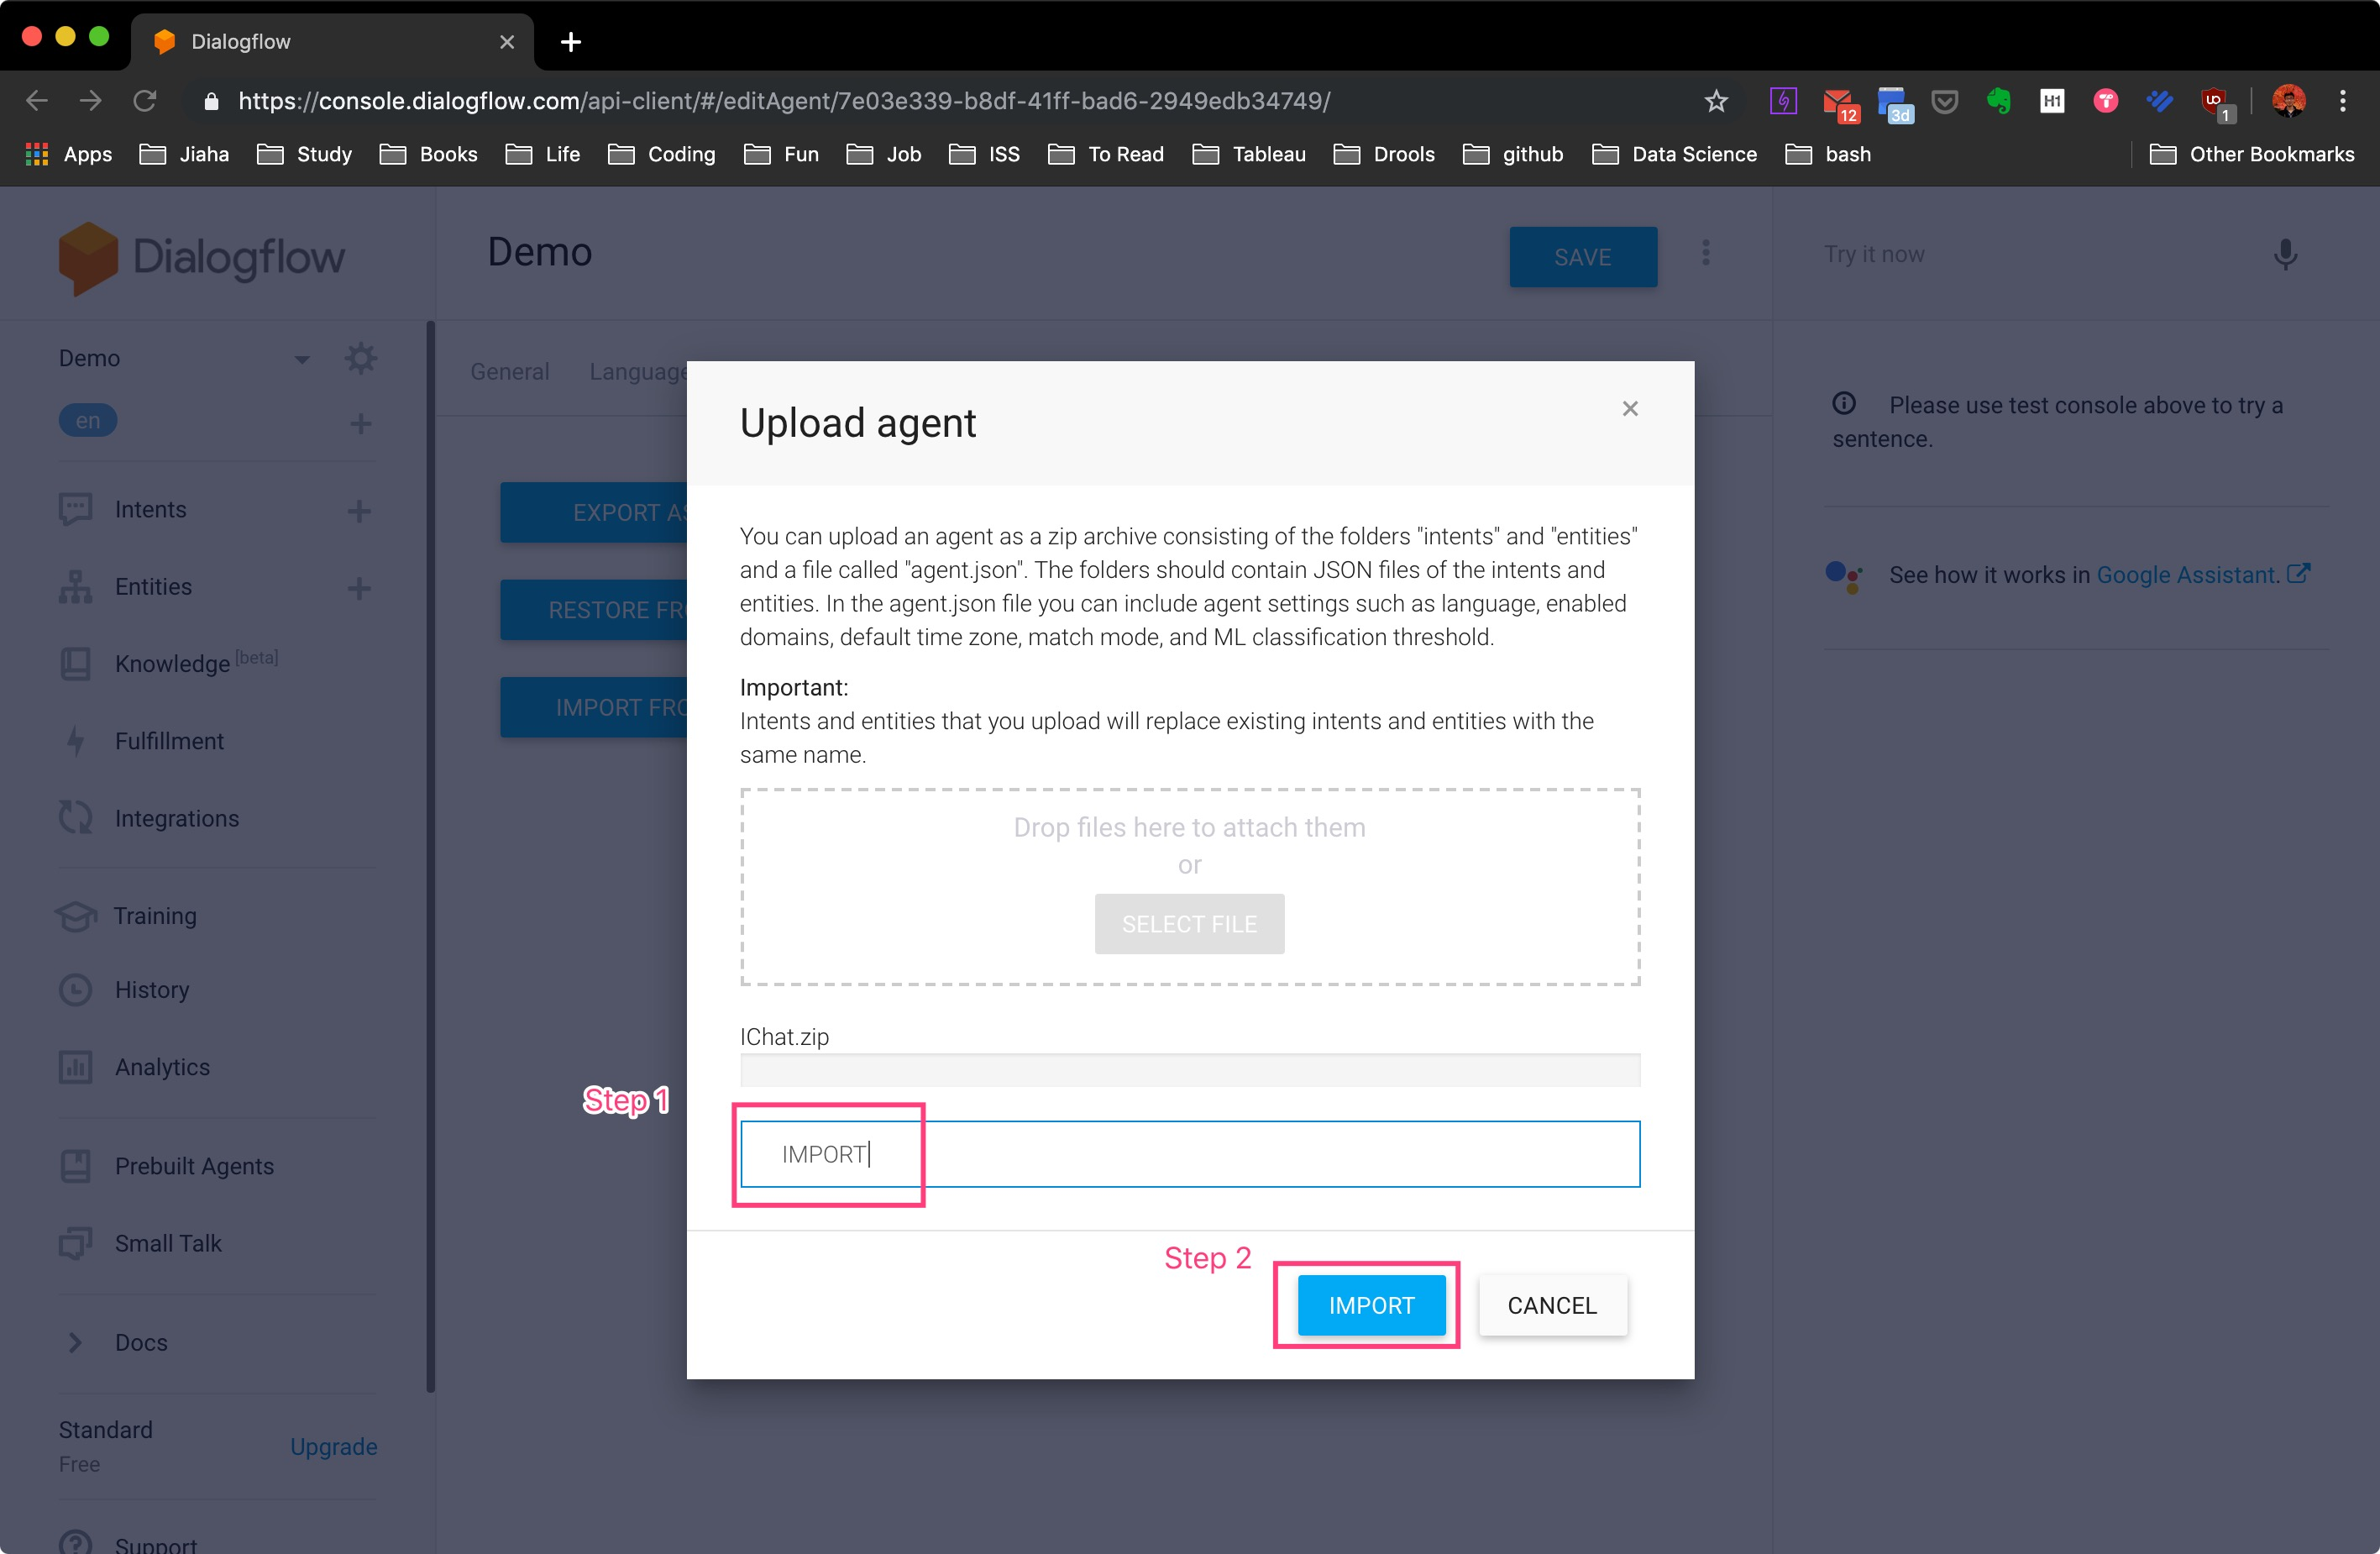
\includegraphics[width=\linewidth, frame]{img/manual_6.jpg}
	\end{figure}
\end{enumerate}
% section import_agent (end)

So far the “Intent” and “Entities” should be all imported into this agent.
Let’s continue to import “knowledge”.

\section{Create Knowledge} % (fold)
\label{sec:create_knowledge}
\begin{enumerate}

	\item Click “Knowledge” and then “Create the first one”

	\begin{figure}[H]
		\centering
		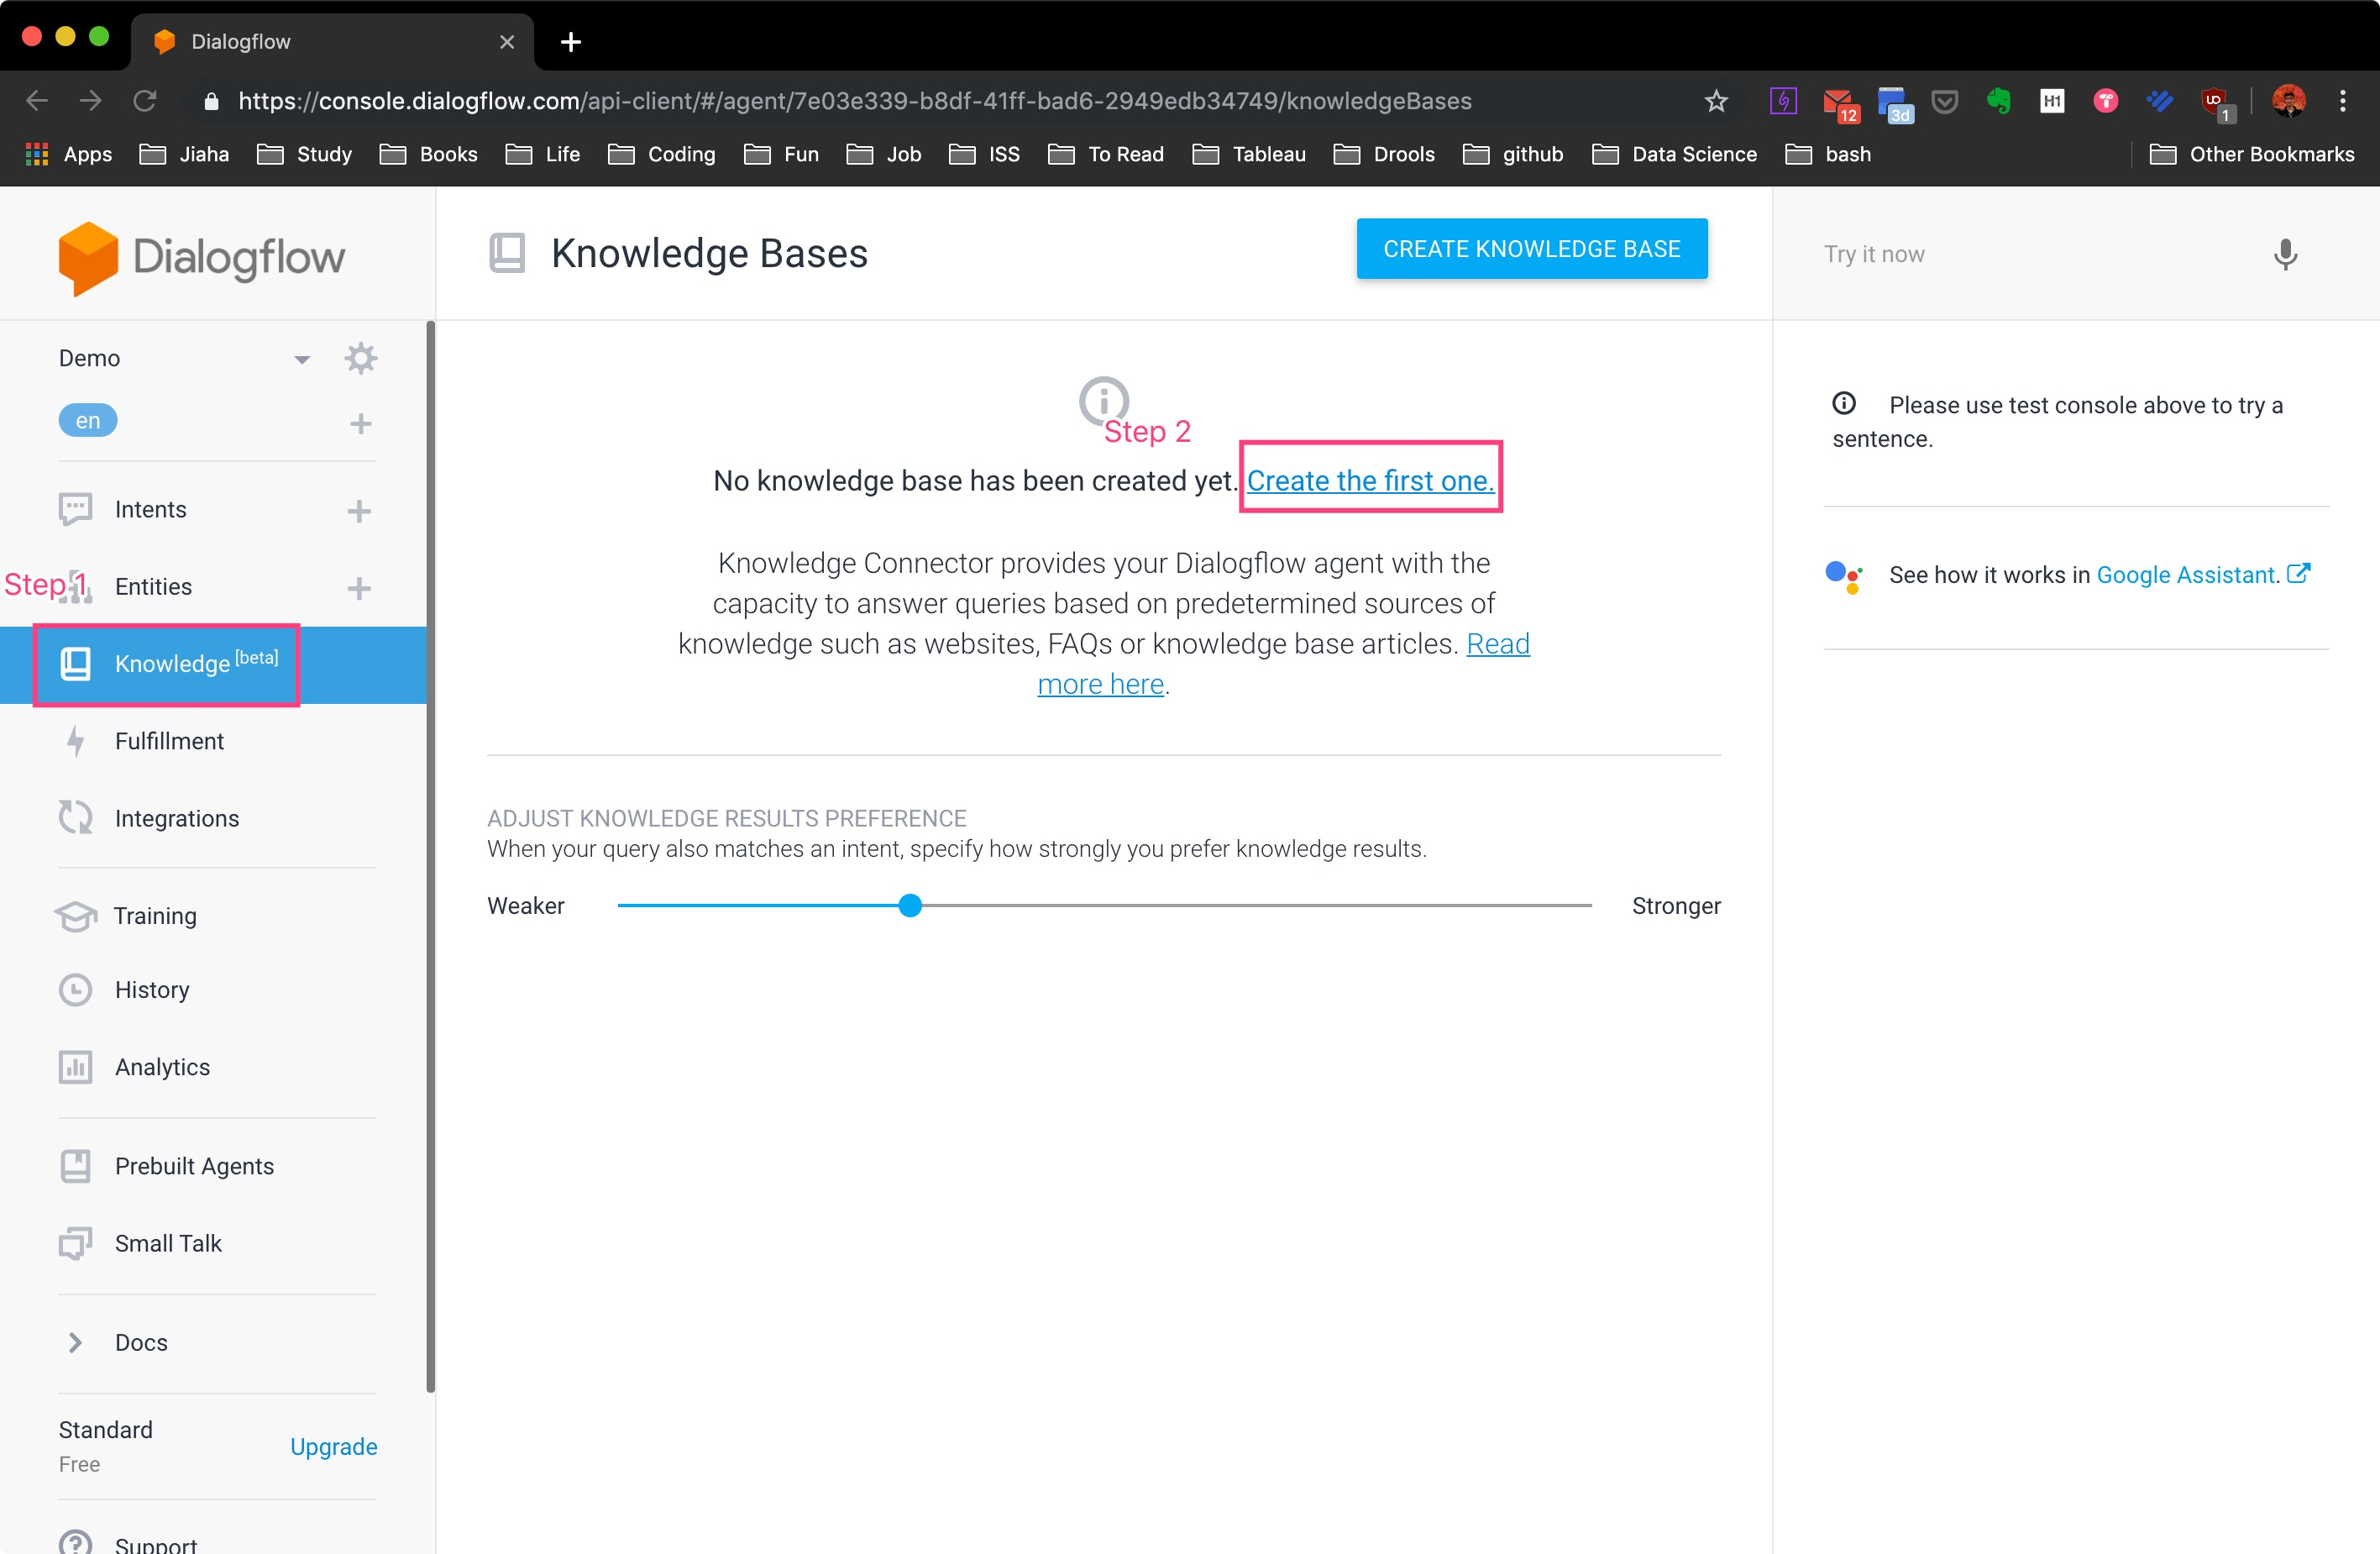
\includegraphics[width=\linewidth, frame]{img/manual_7.jpg}
	\end{figure}

	\item Put Agent name as you wish, then click “SAVE” button

	\begin{figure}[H]
		\centering
		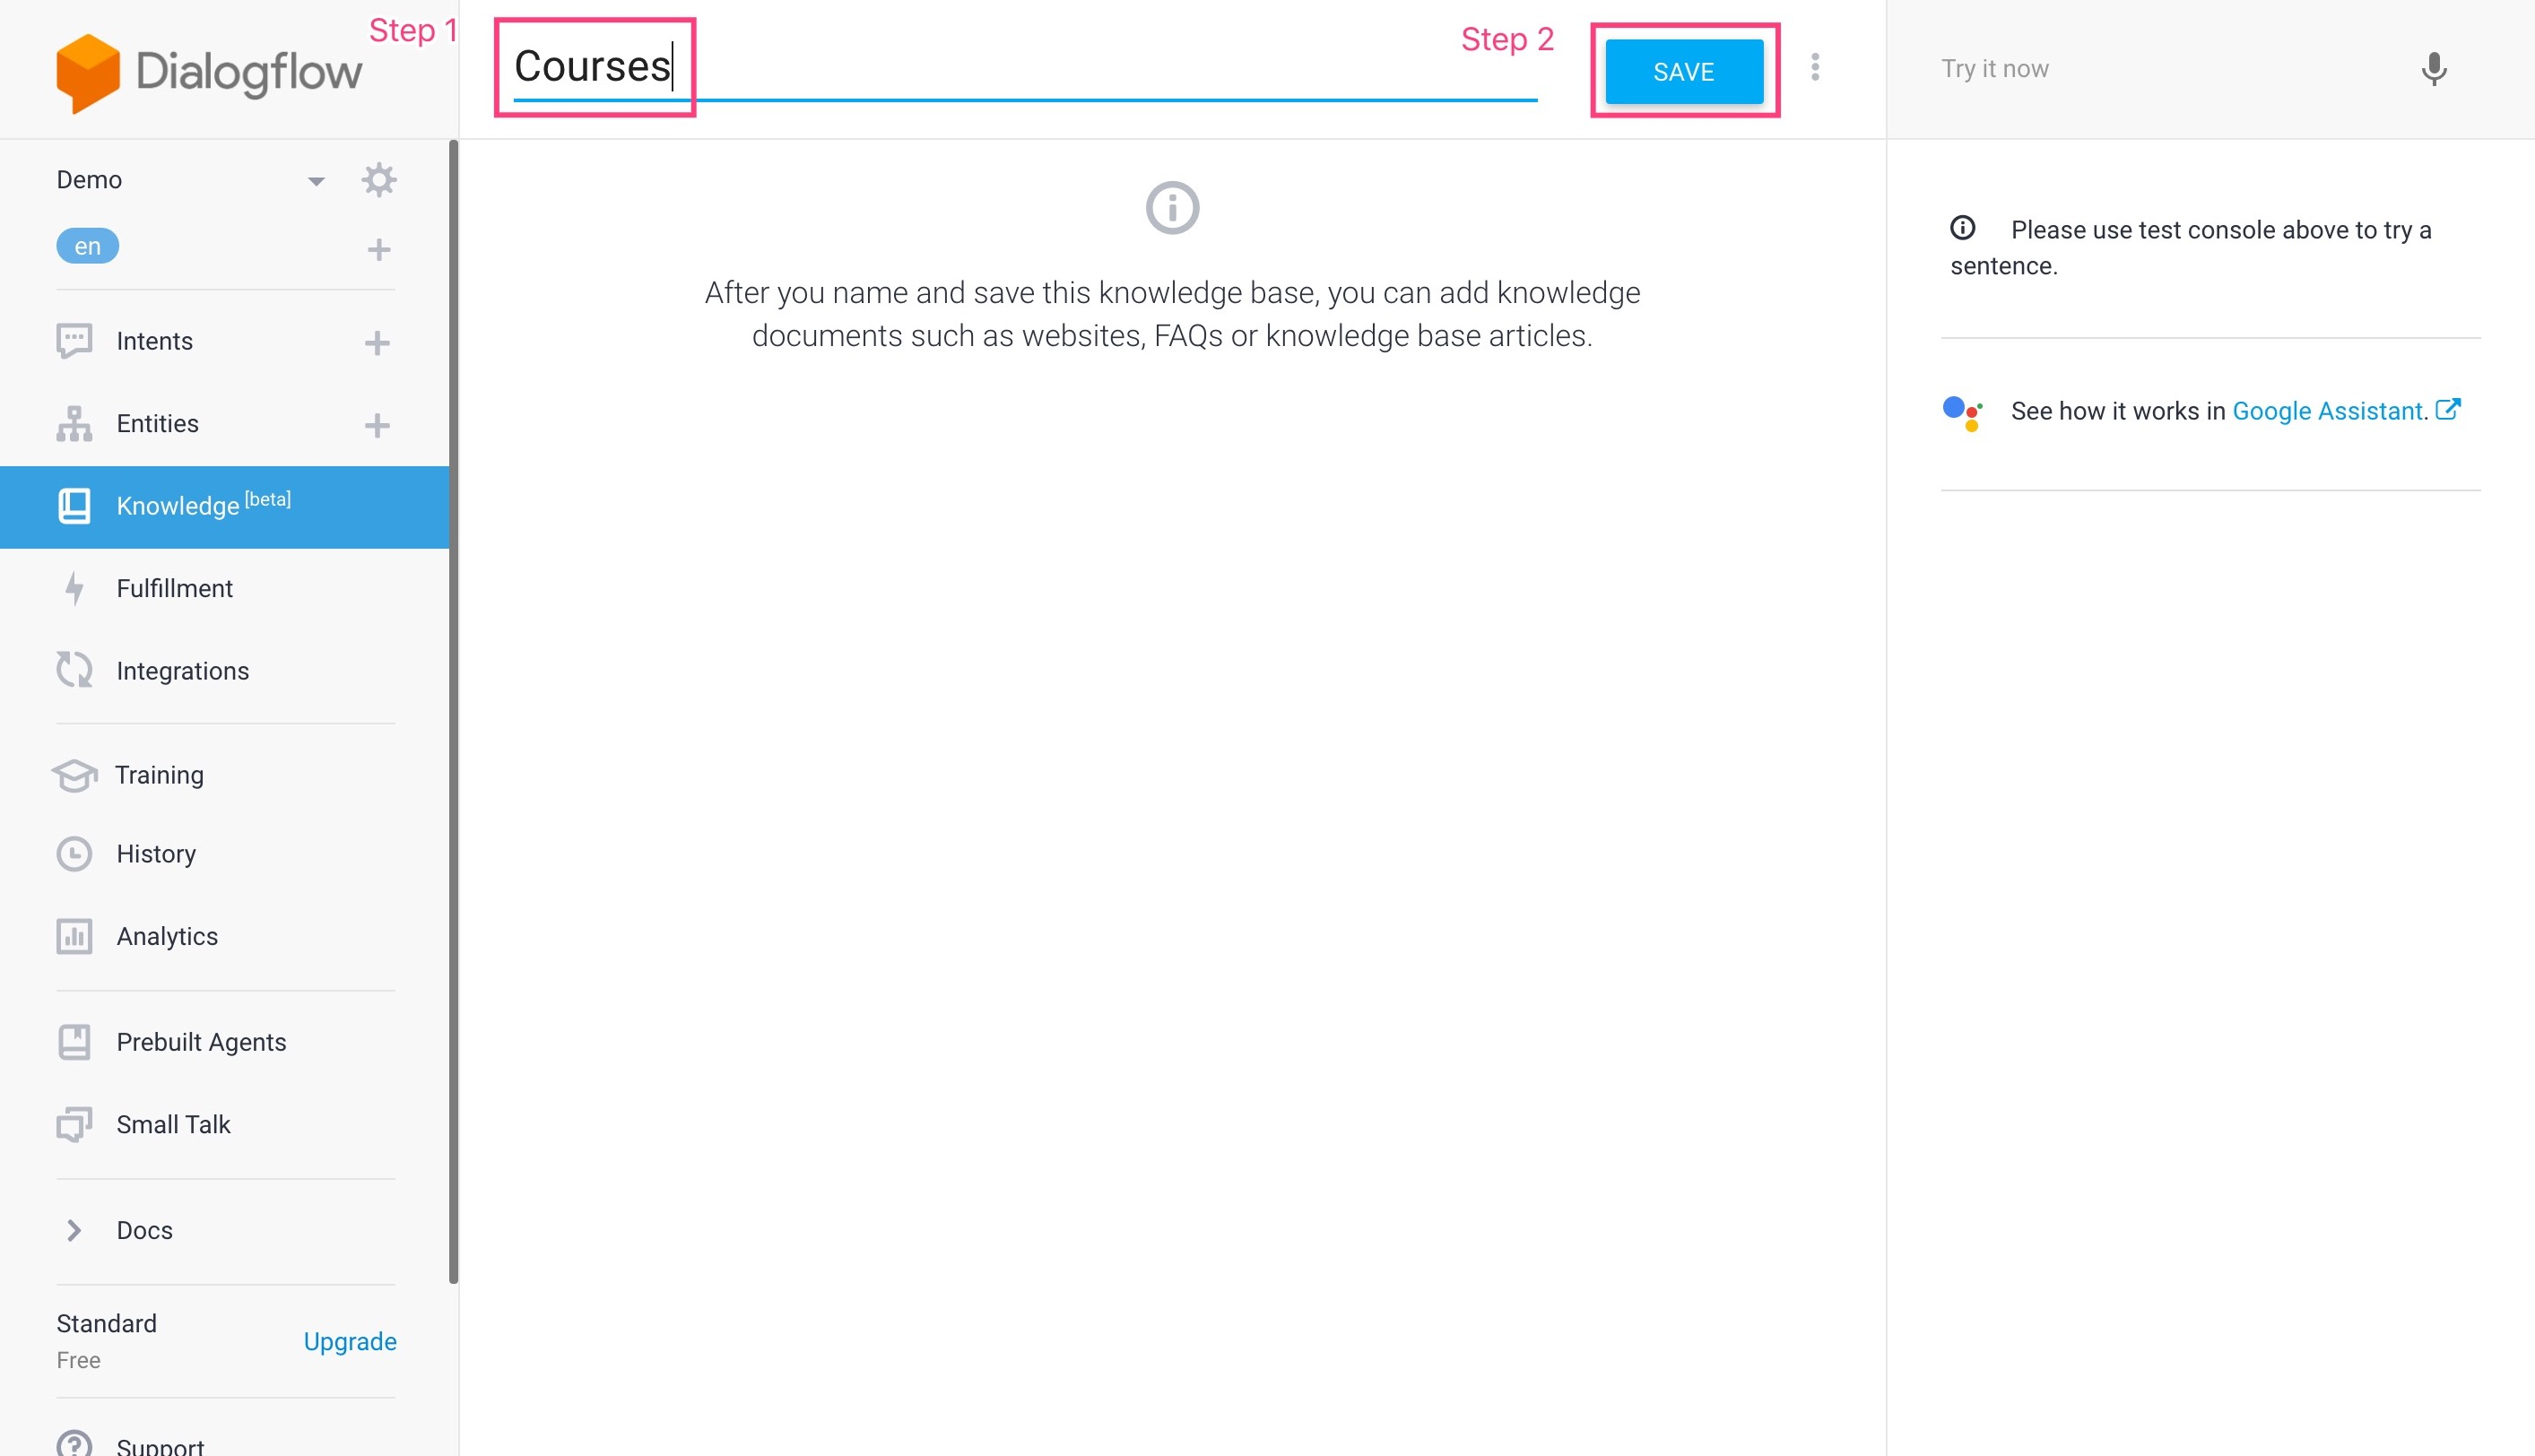
\includegraphics[width=\linewidth, frame]{img/manual_8.jpg}
	\end{figure}

	\item Click “Create the first one”
	\nopagebreak
	\begin{figure}[H]
		\centering
		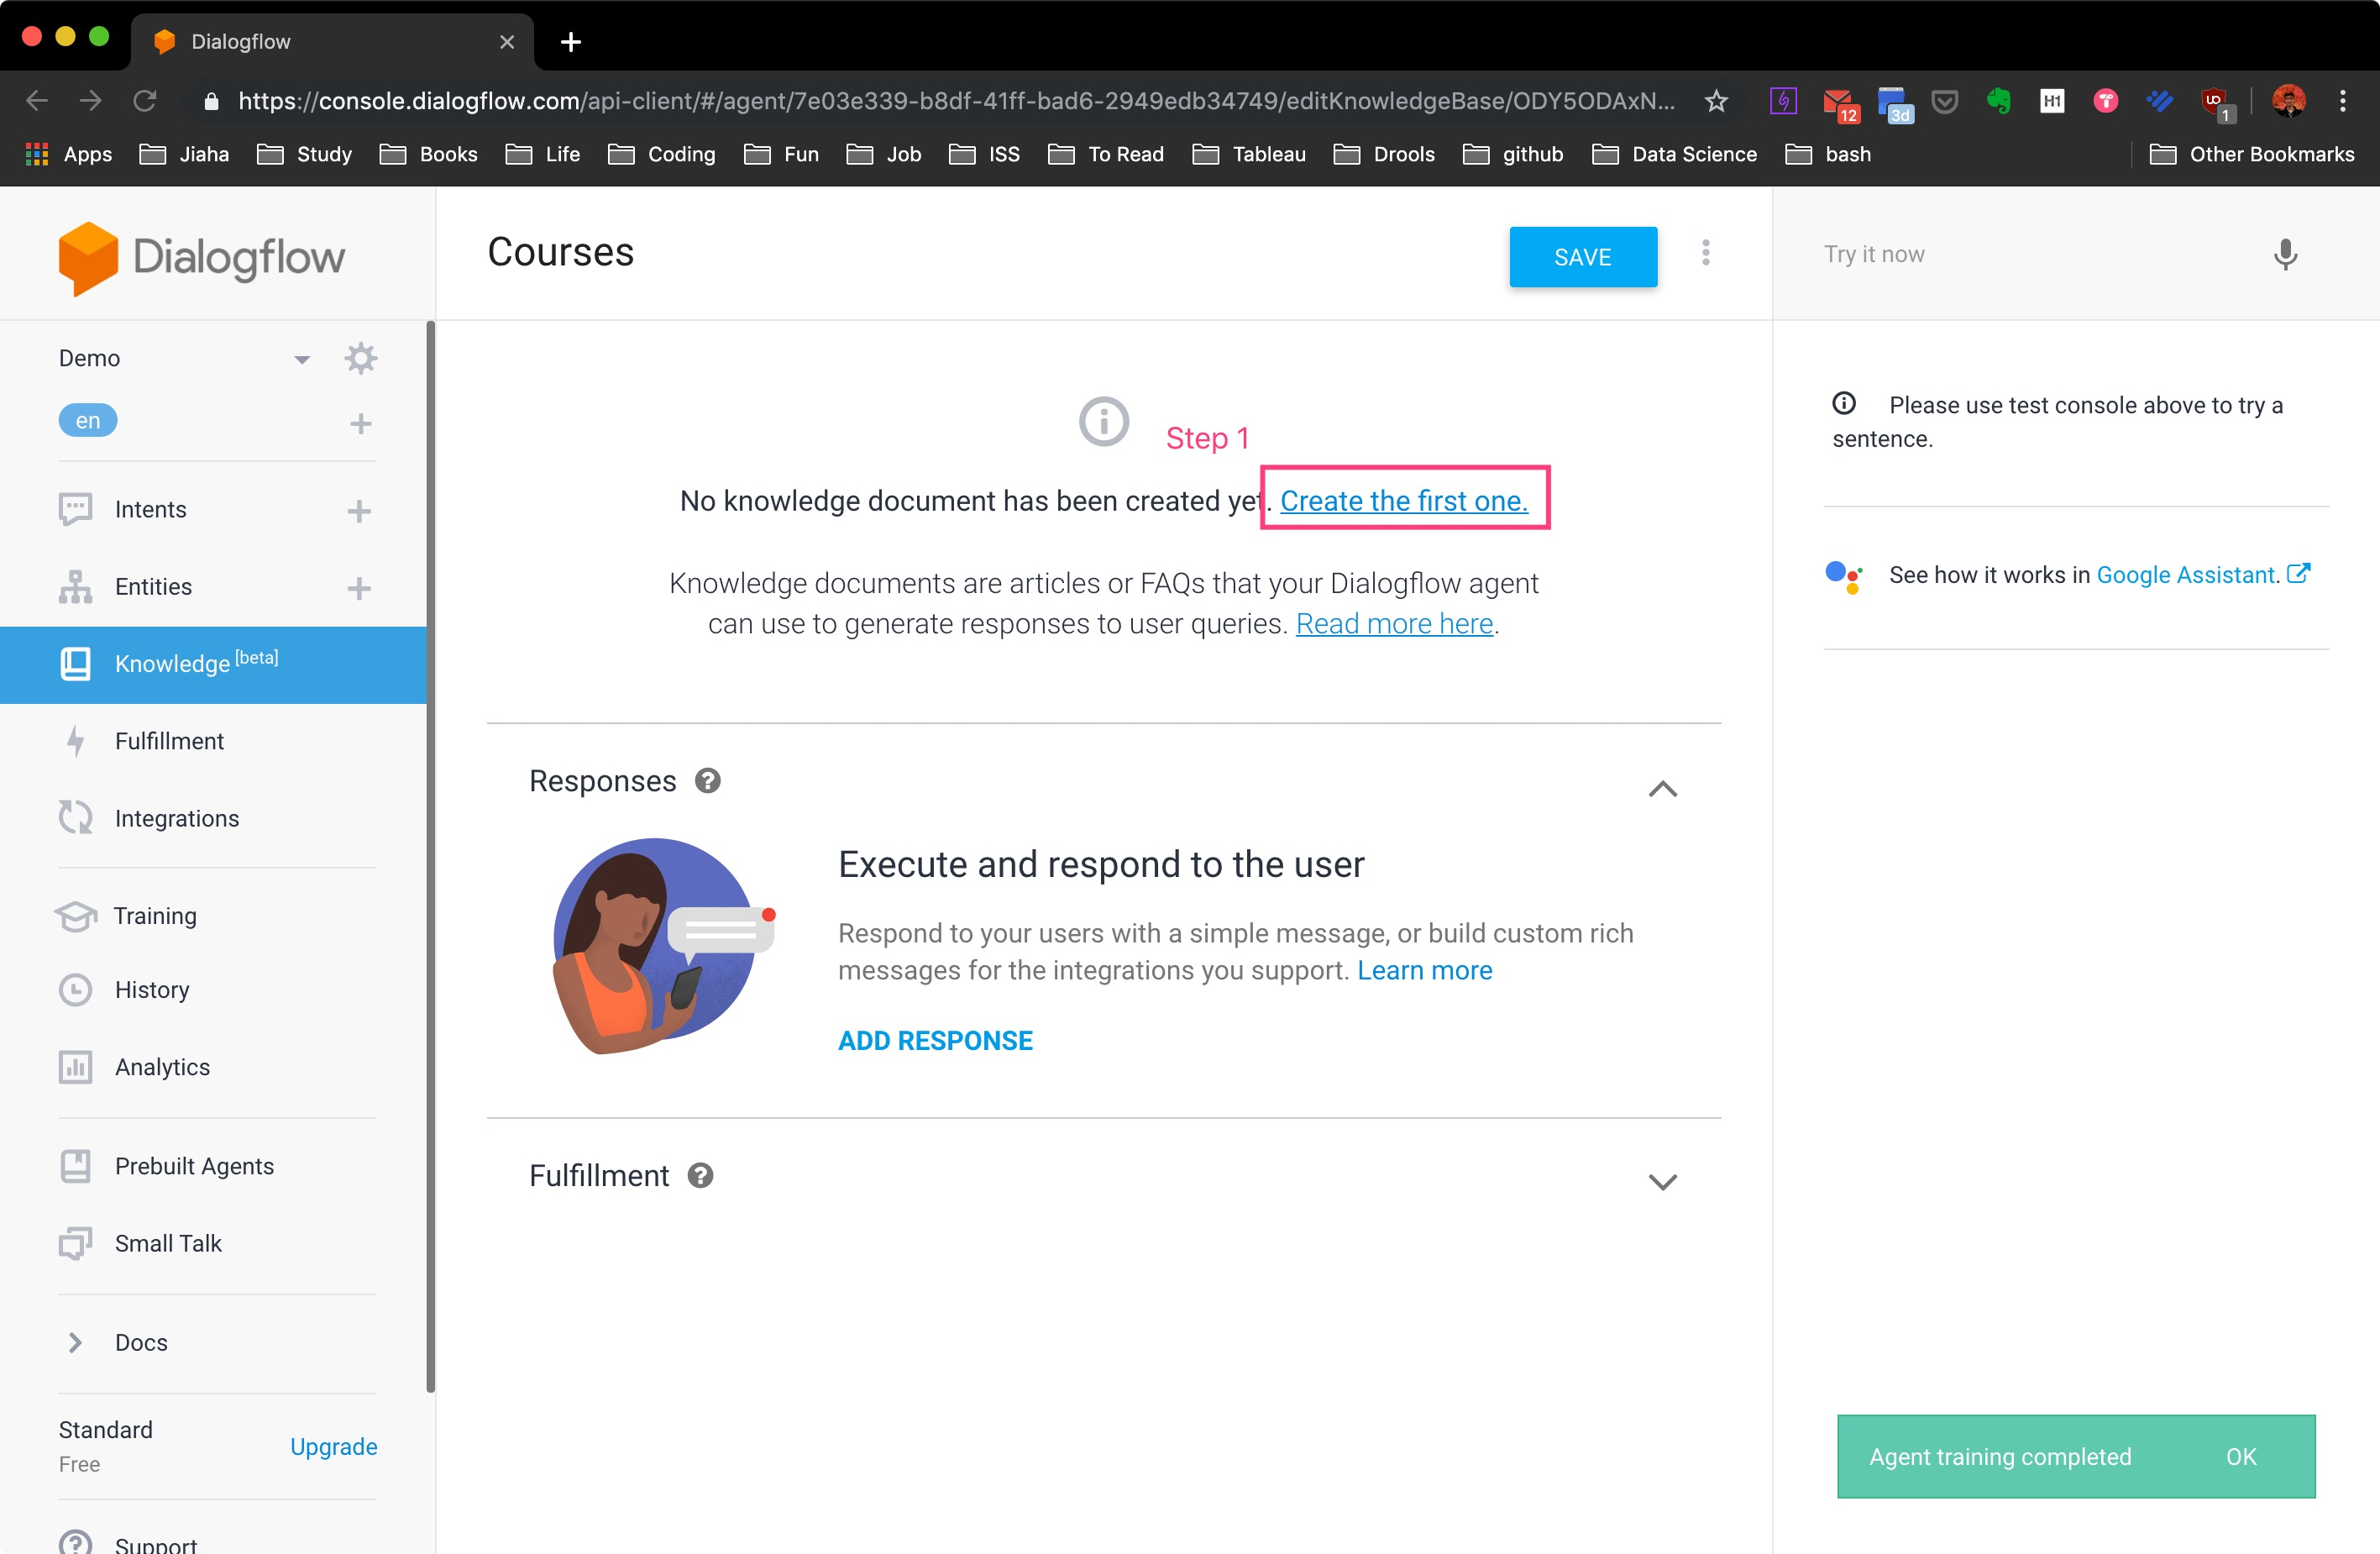
\includegraphics[width=\linewidth, frame]{img/manual_9.jpg}
	\end{figure}

	\item Input the fields as follows and upload “part1.csv”, then click “CREATE” button
	\nopagebreak
	\begin{figure}[H]
		\centering
		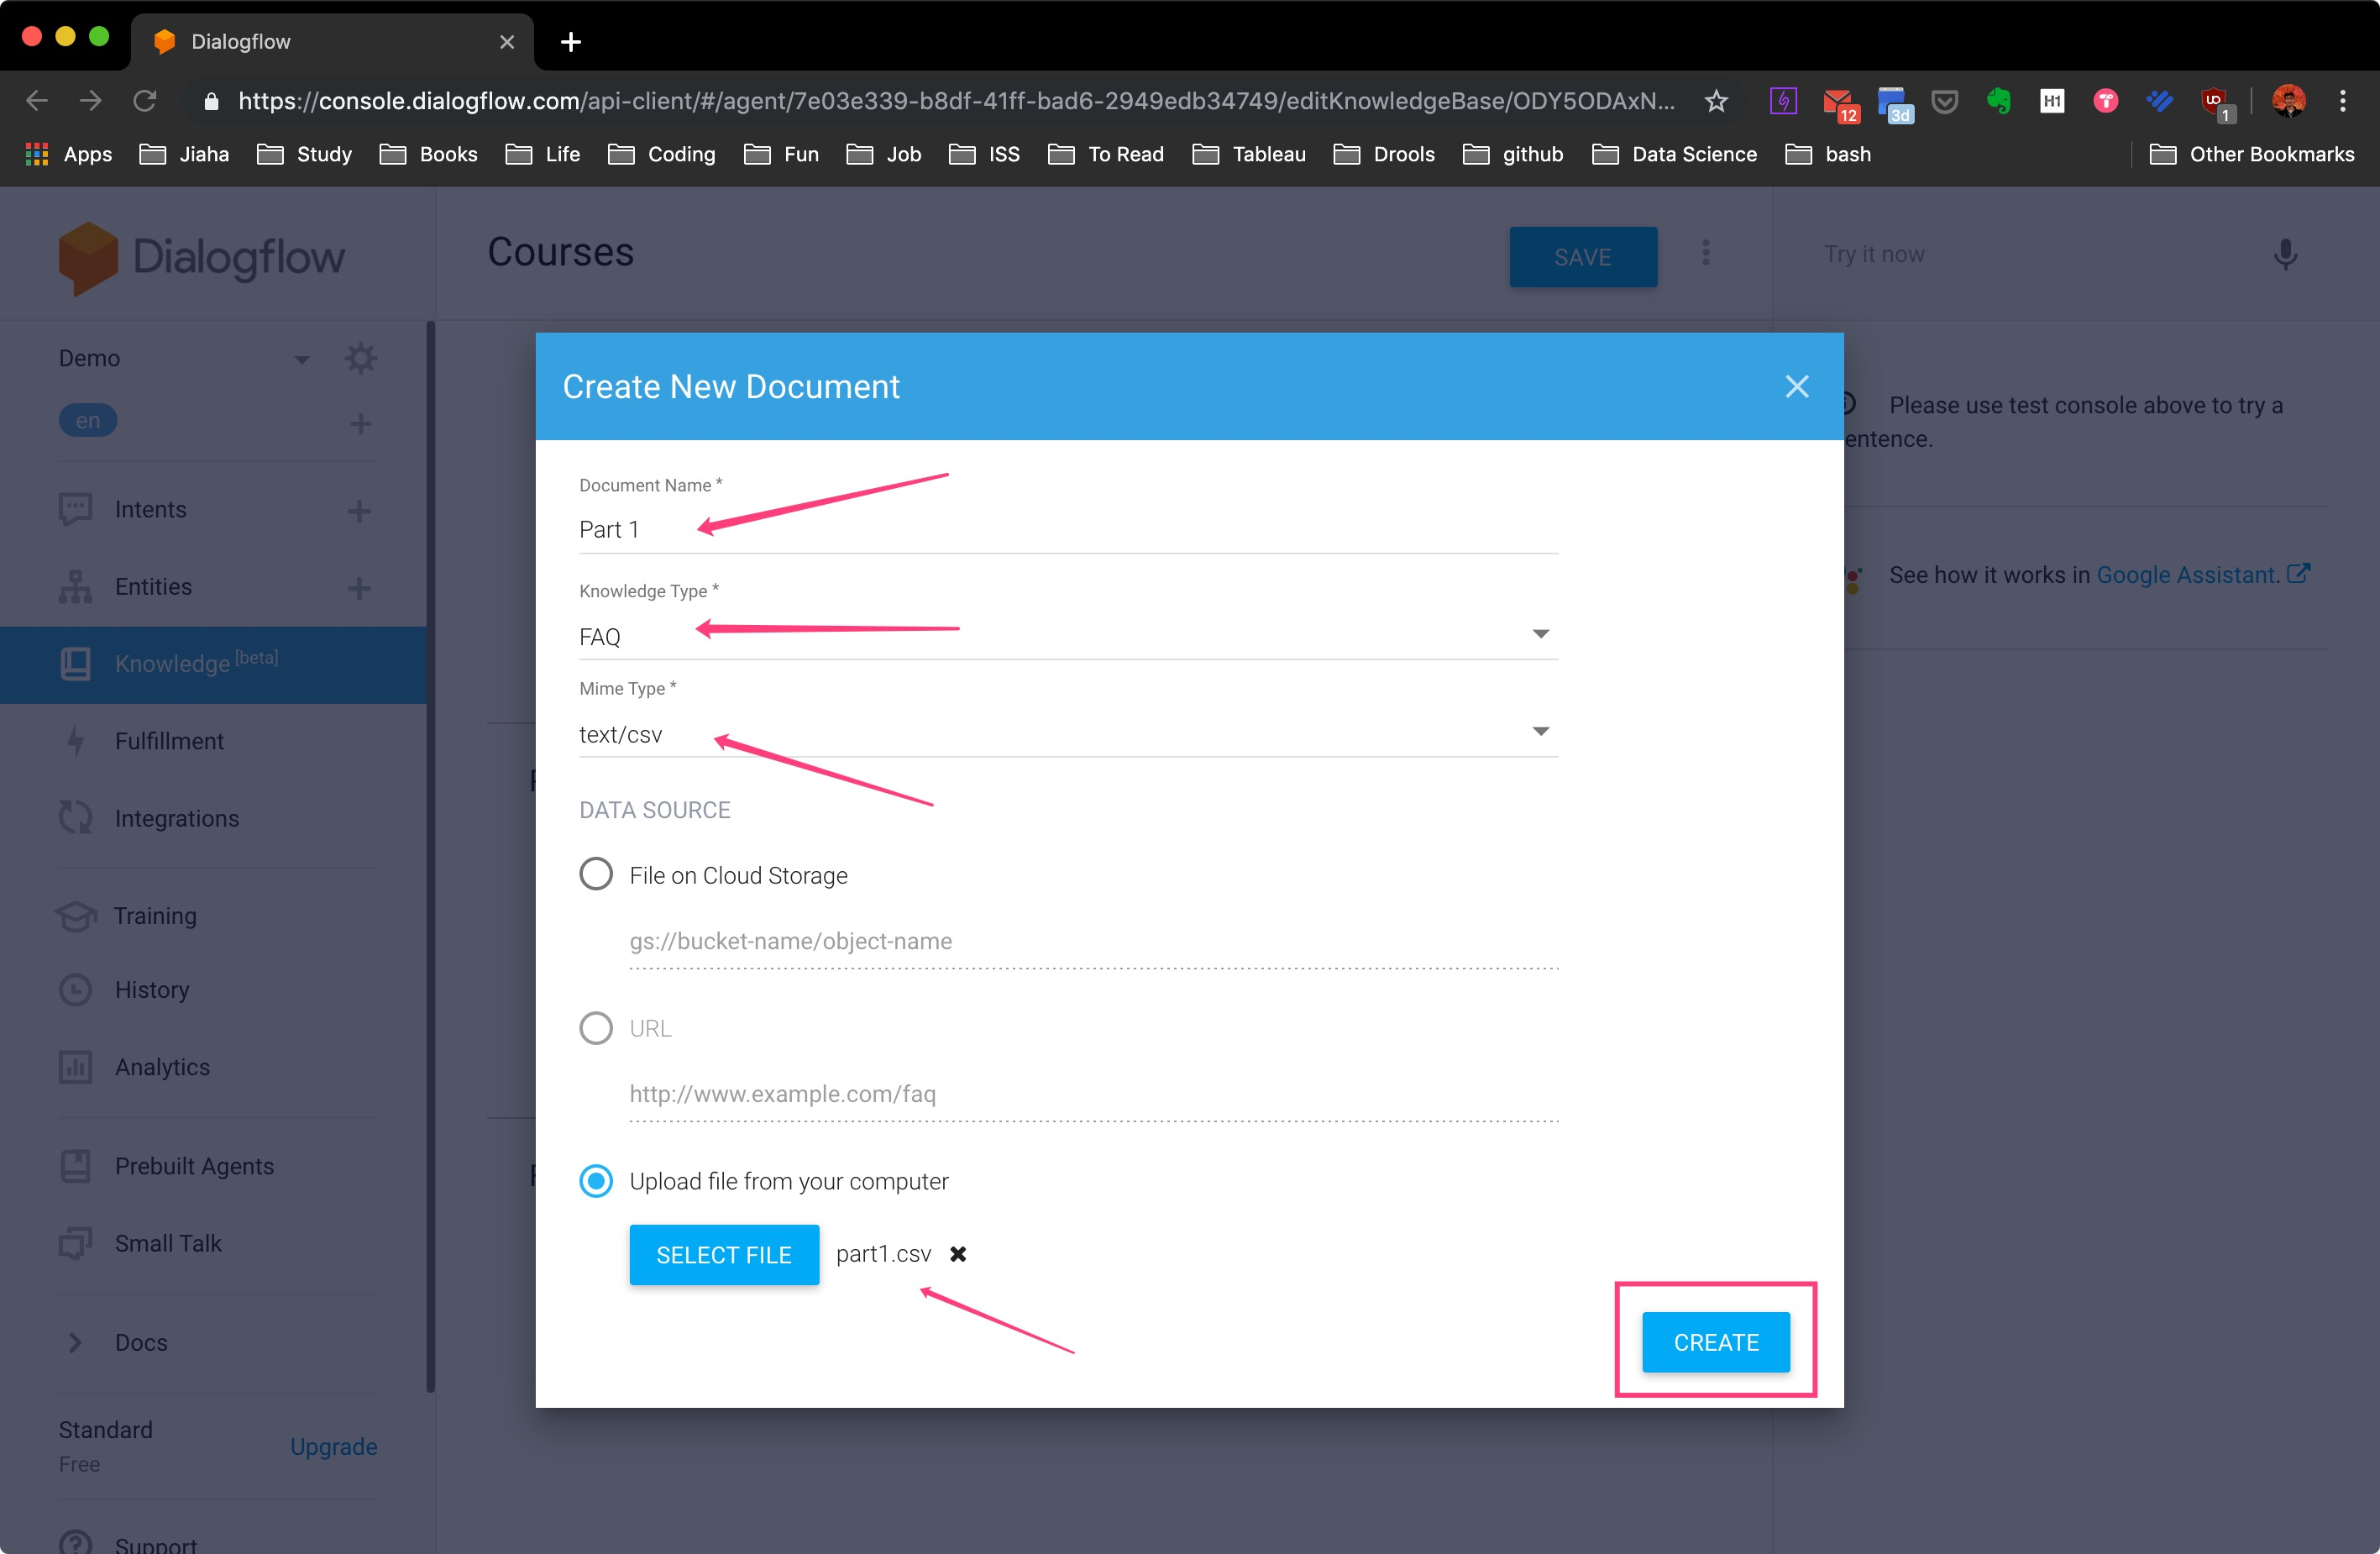
\includegraphics[width=\linewidth, frame]{img/manual_10.jpg}
	\end{figure}

	\item Click “+ New Document”
	\nopagebreak
	\begin{figure}[H]
		\centering
		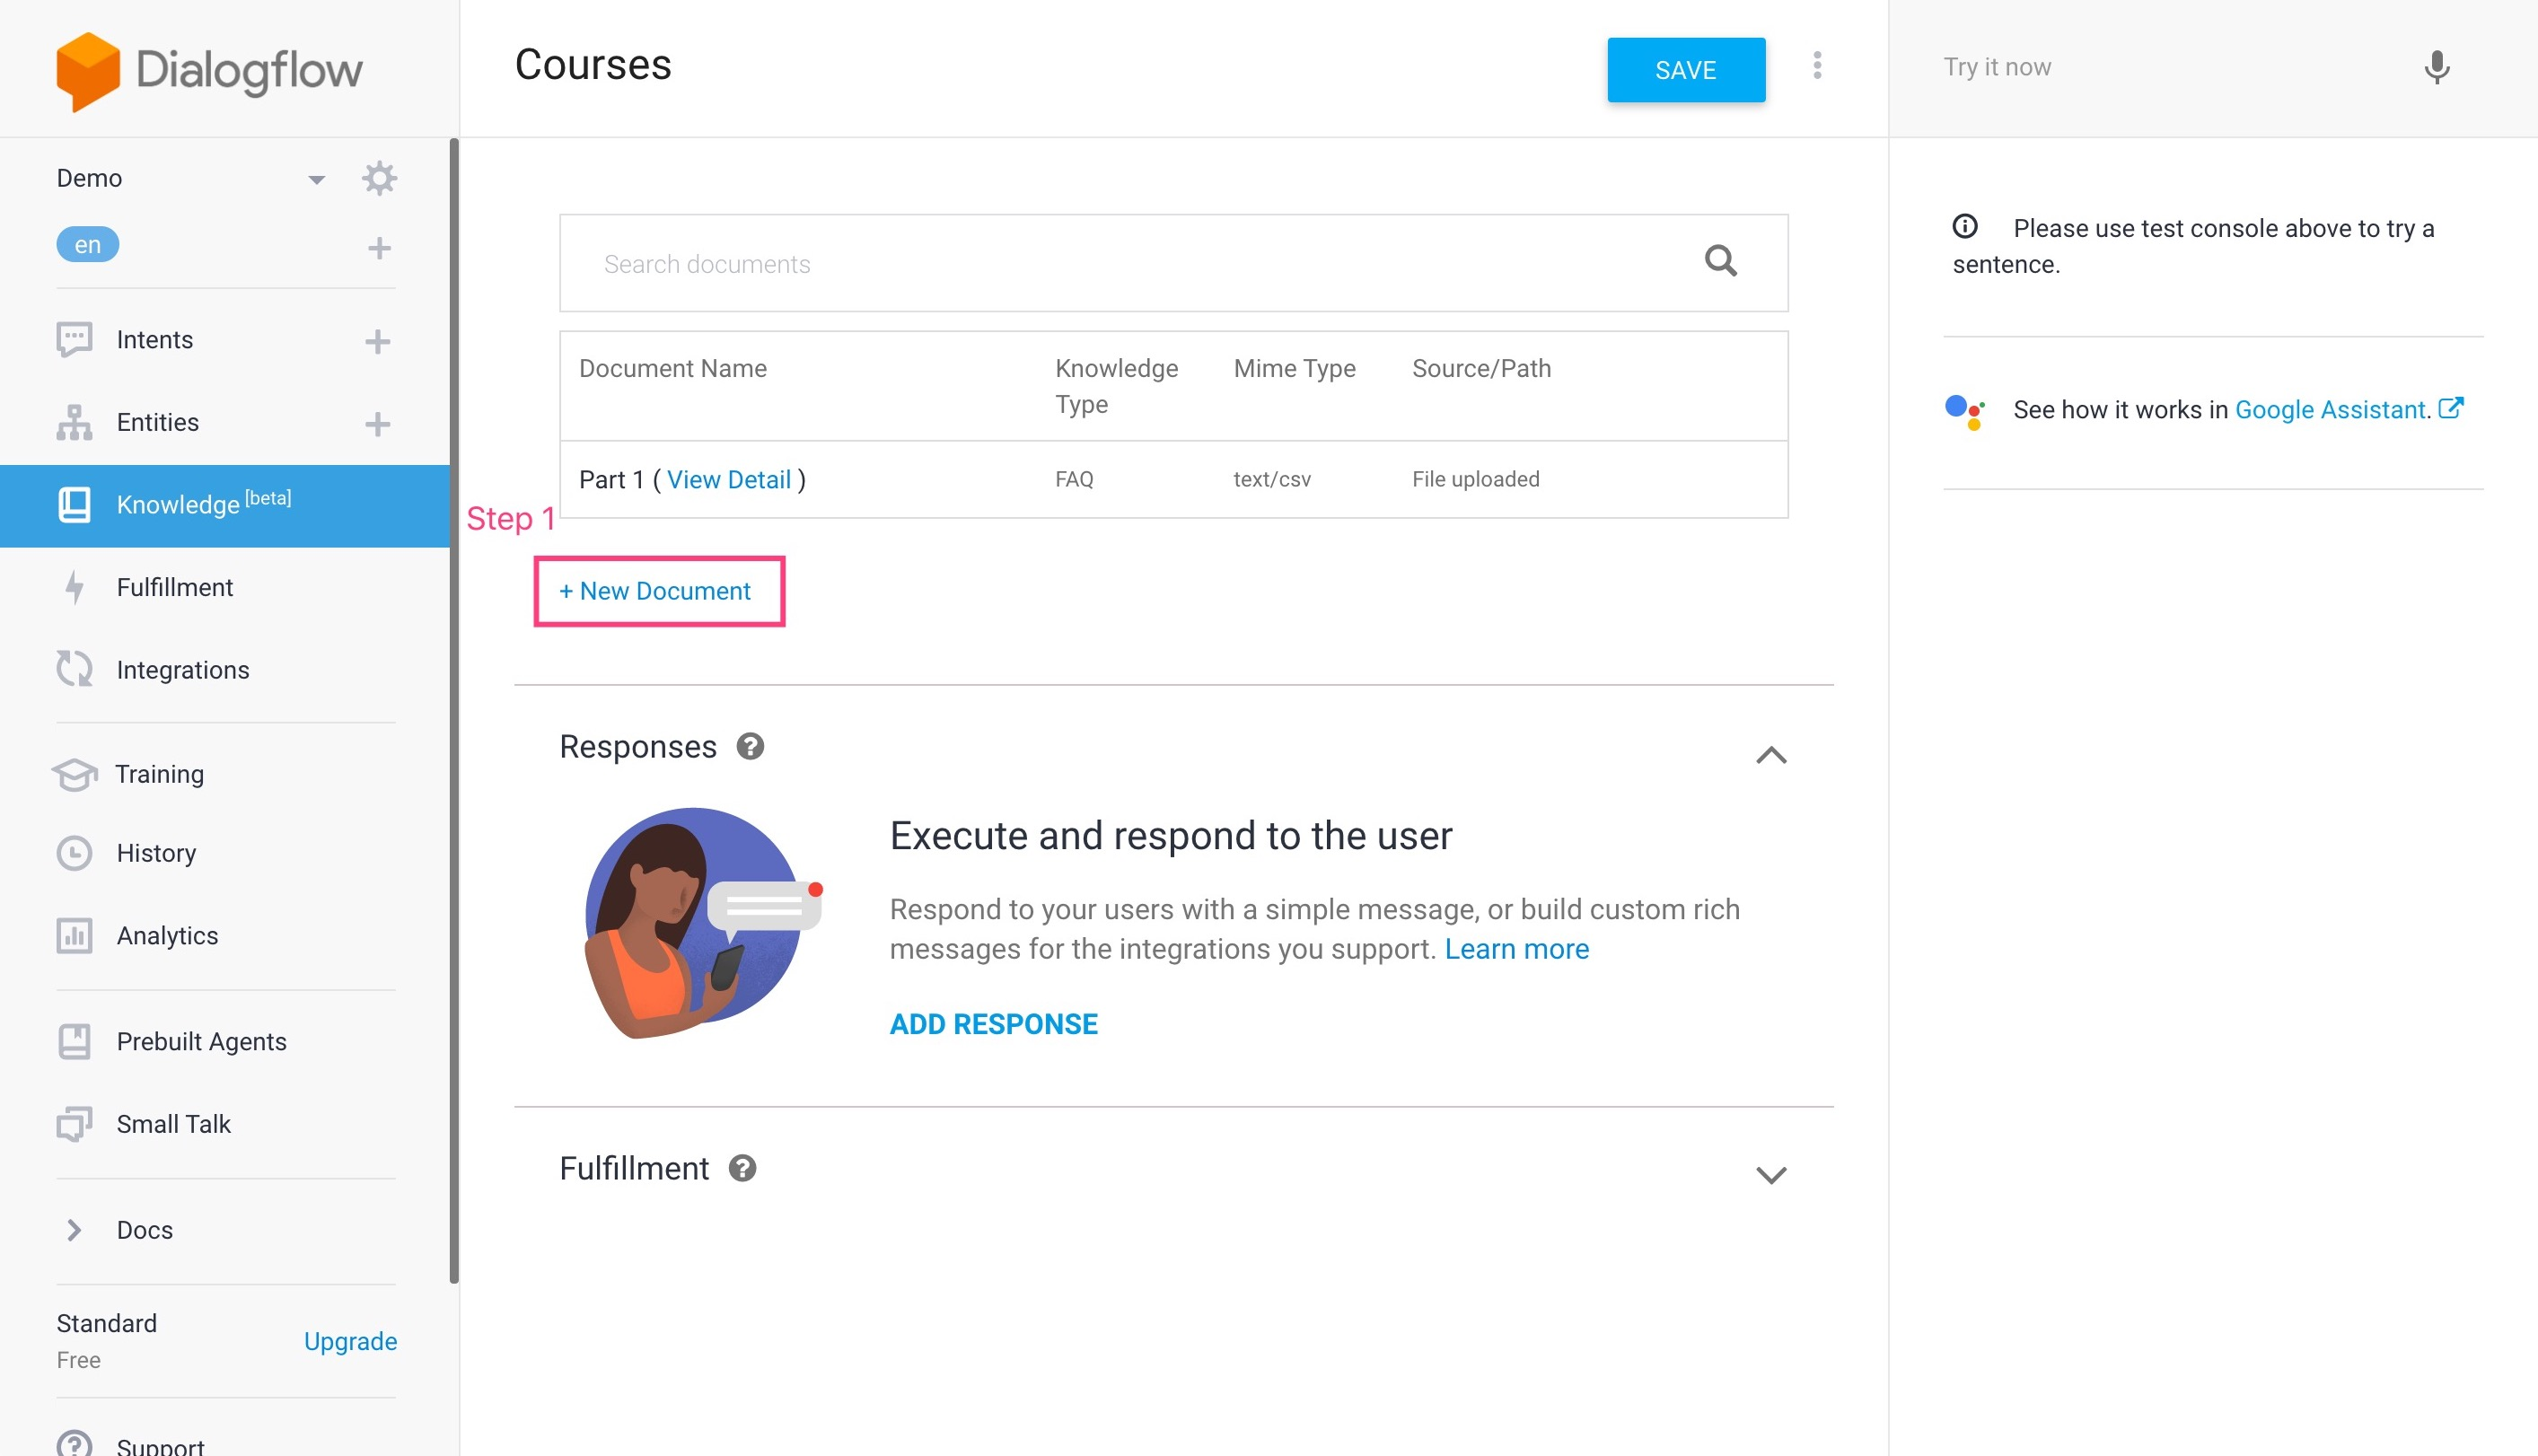
\includegraphics[width=\linewidth, frame]{img/manual_11.jpg}
	\end{figure}

	\item Input the fields as follows and upload “part2.csv”, then click “CREATE” button
	\nopagebreak
	\begin{figure}[H]
		\centering
		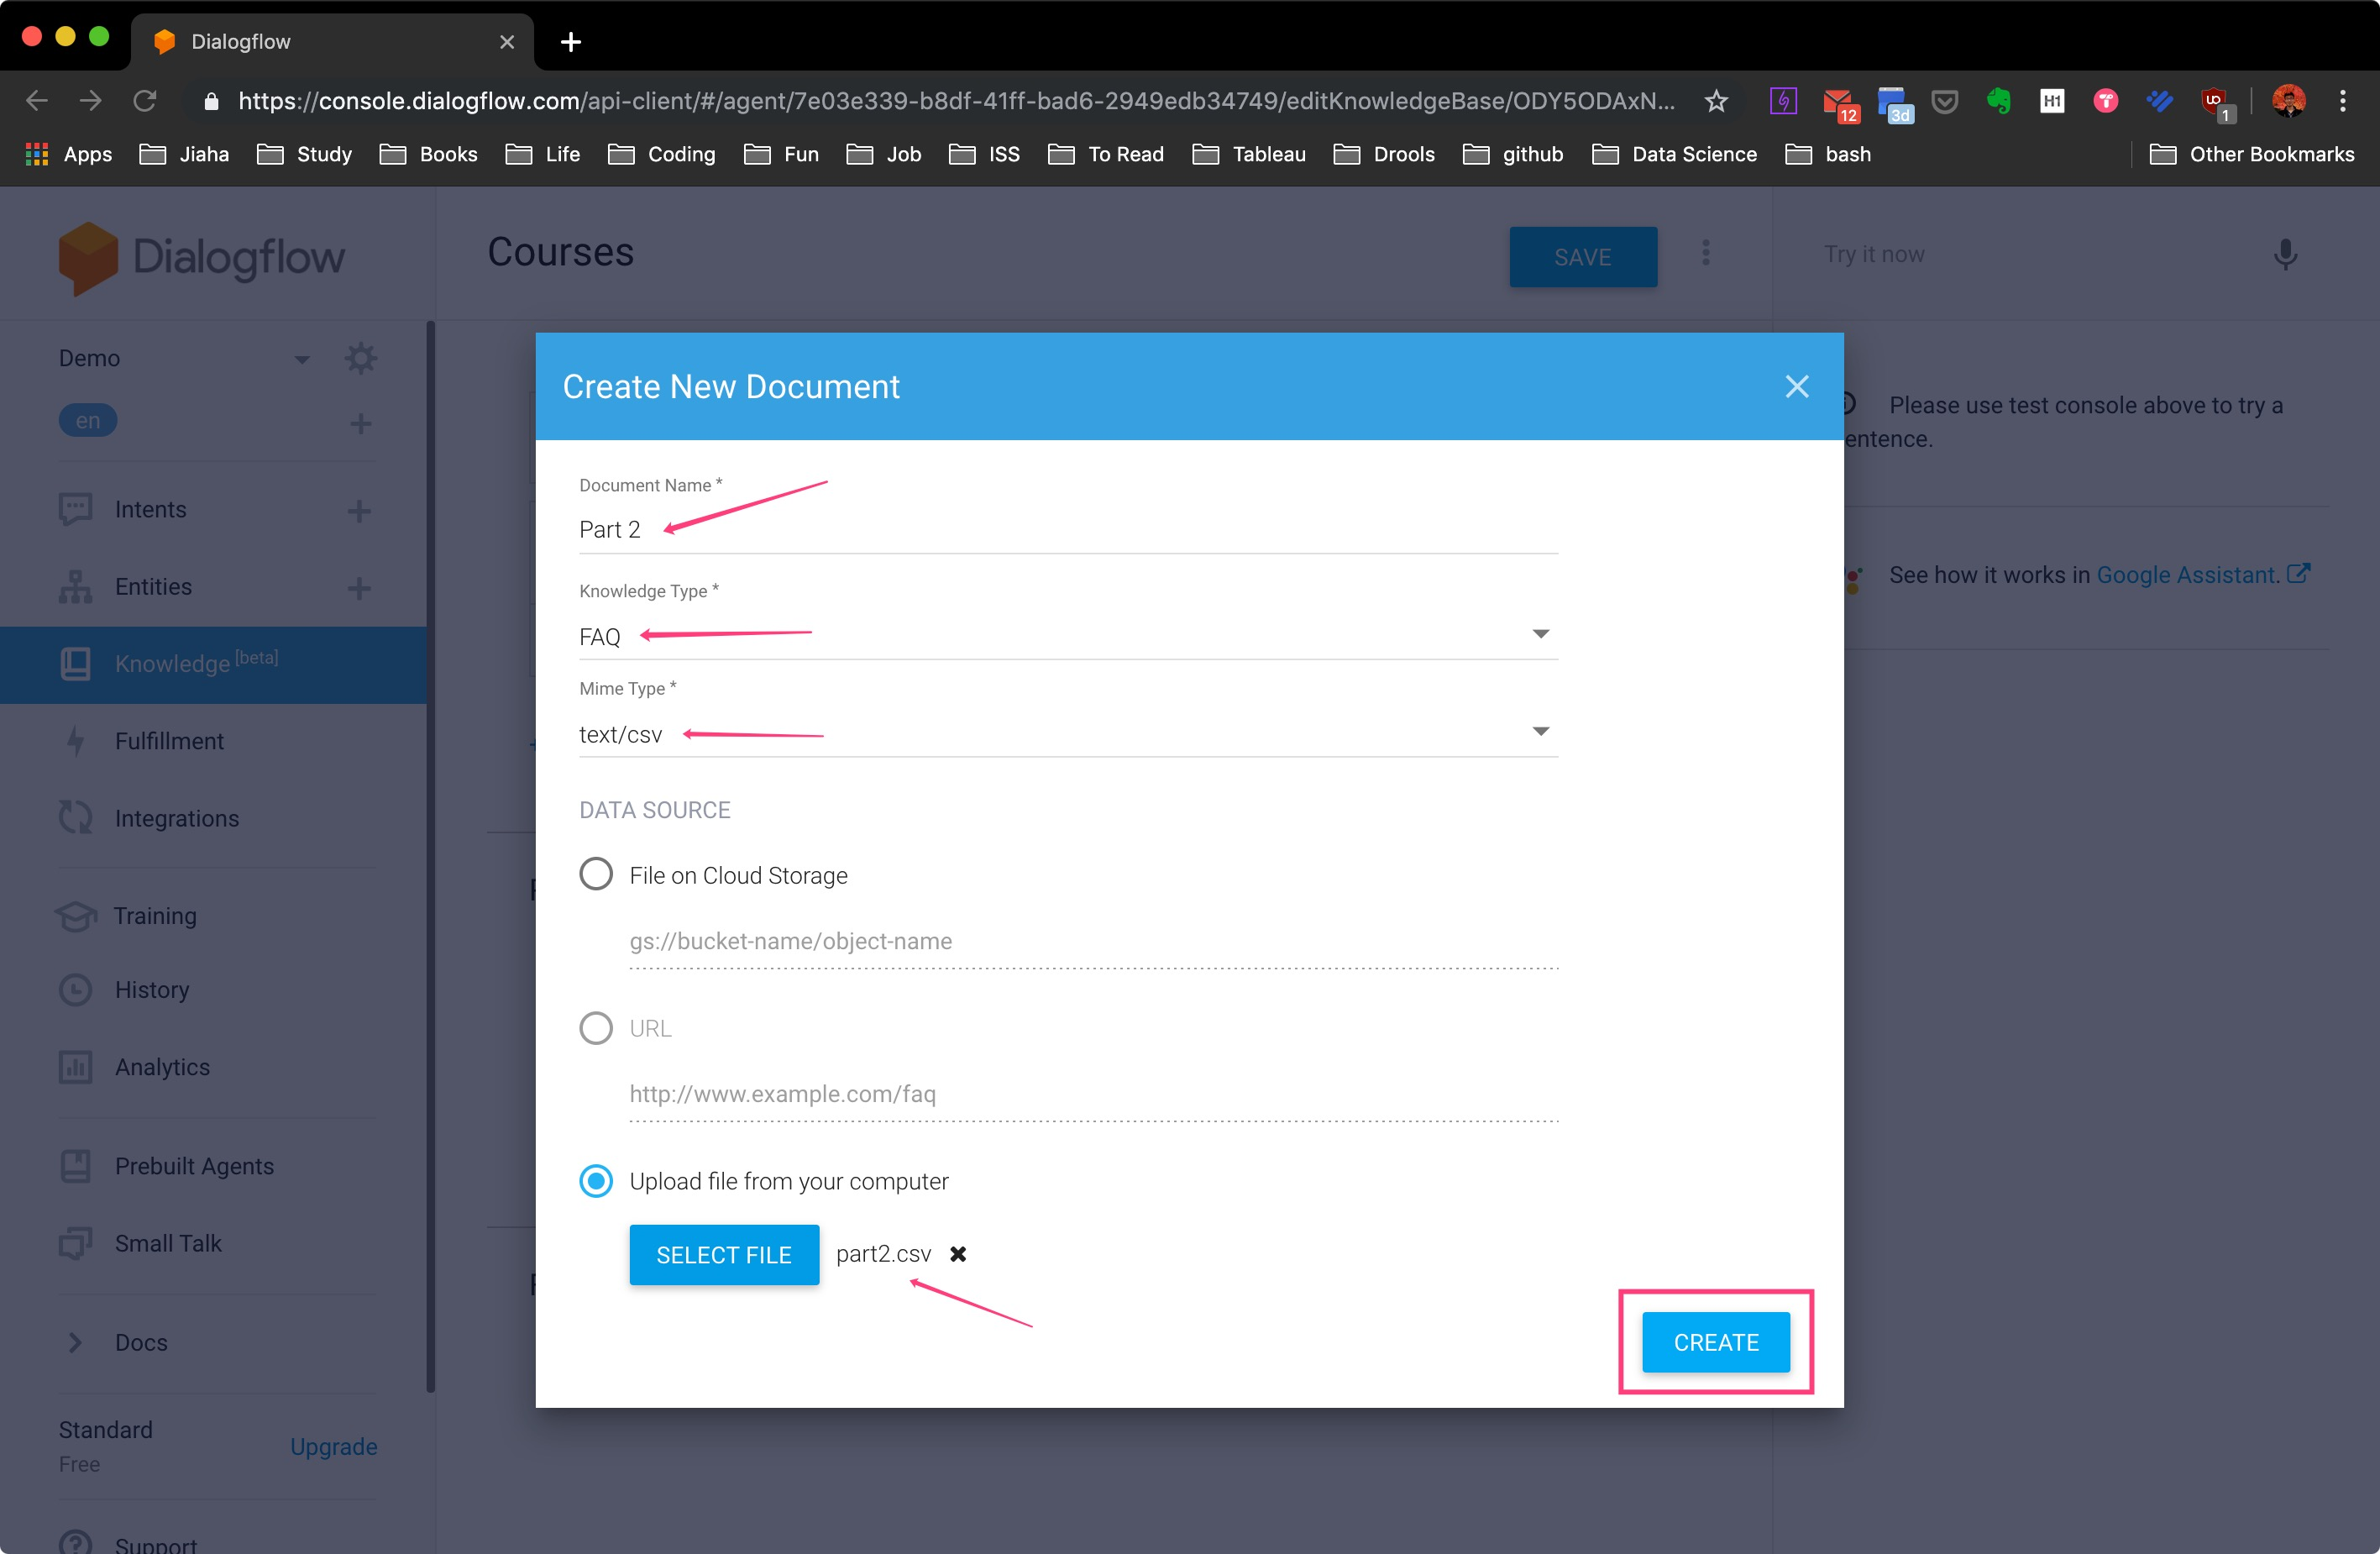
\includegraphics[width=\linewidth, frame]{img/manual_12.jpg}
	\end{figure}

	\item Click “ADD RESPONSE”
	\nopagebreak
	\begin{figure}[H]
		\centering
		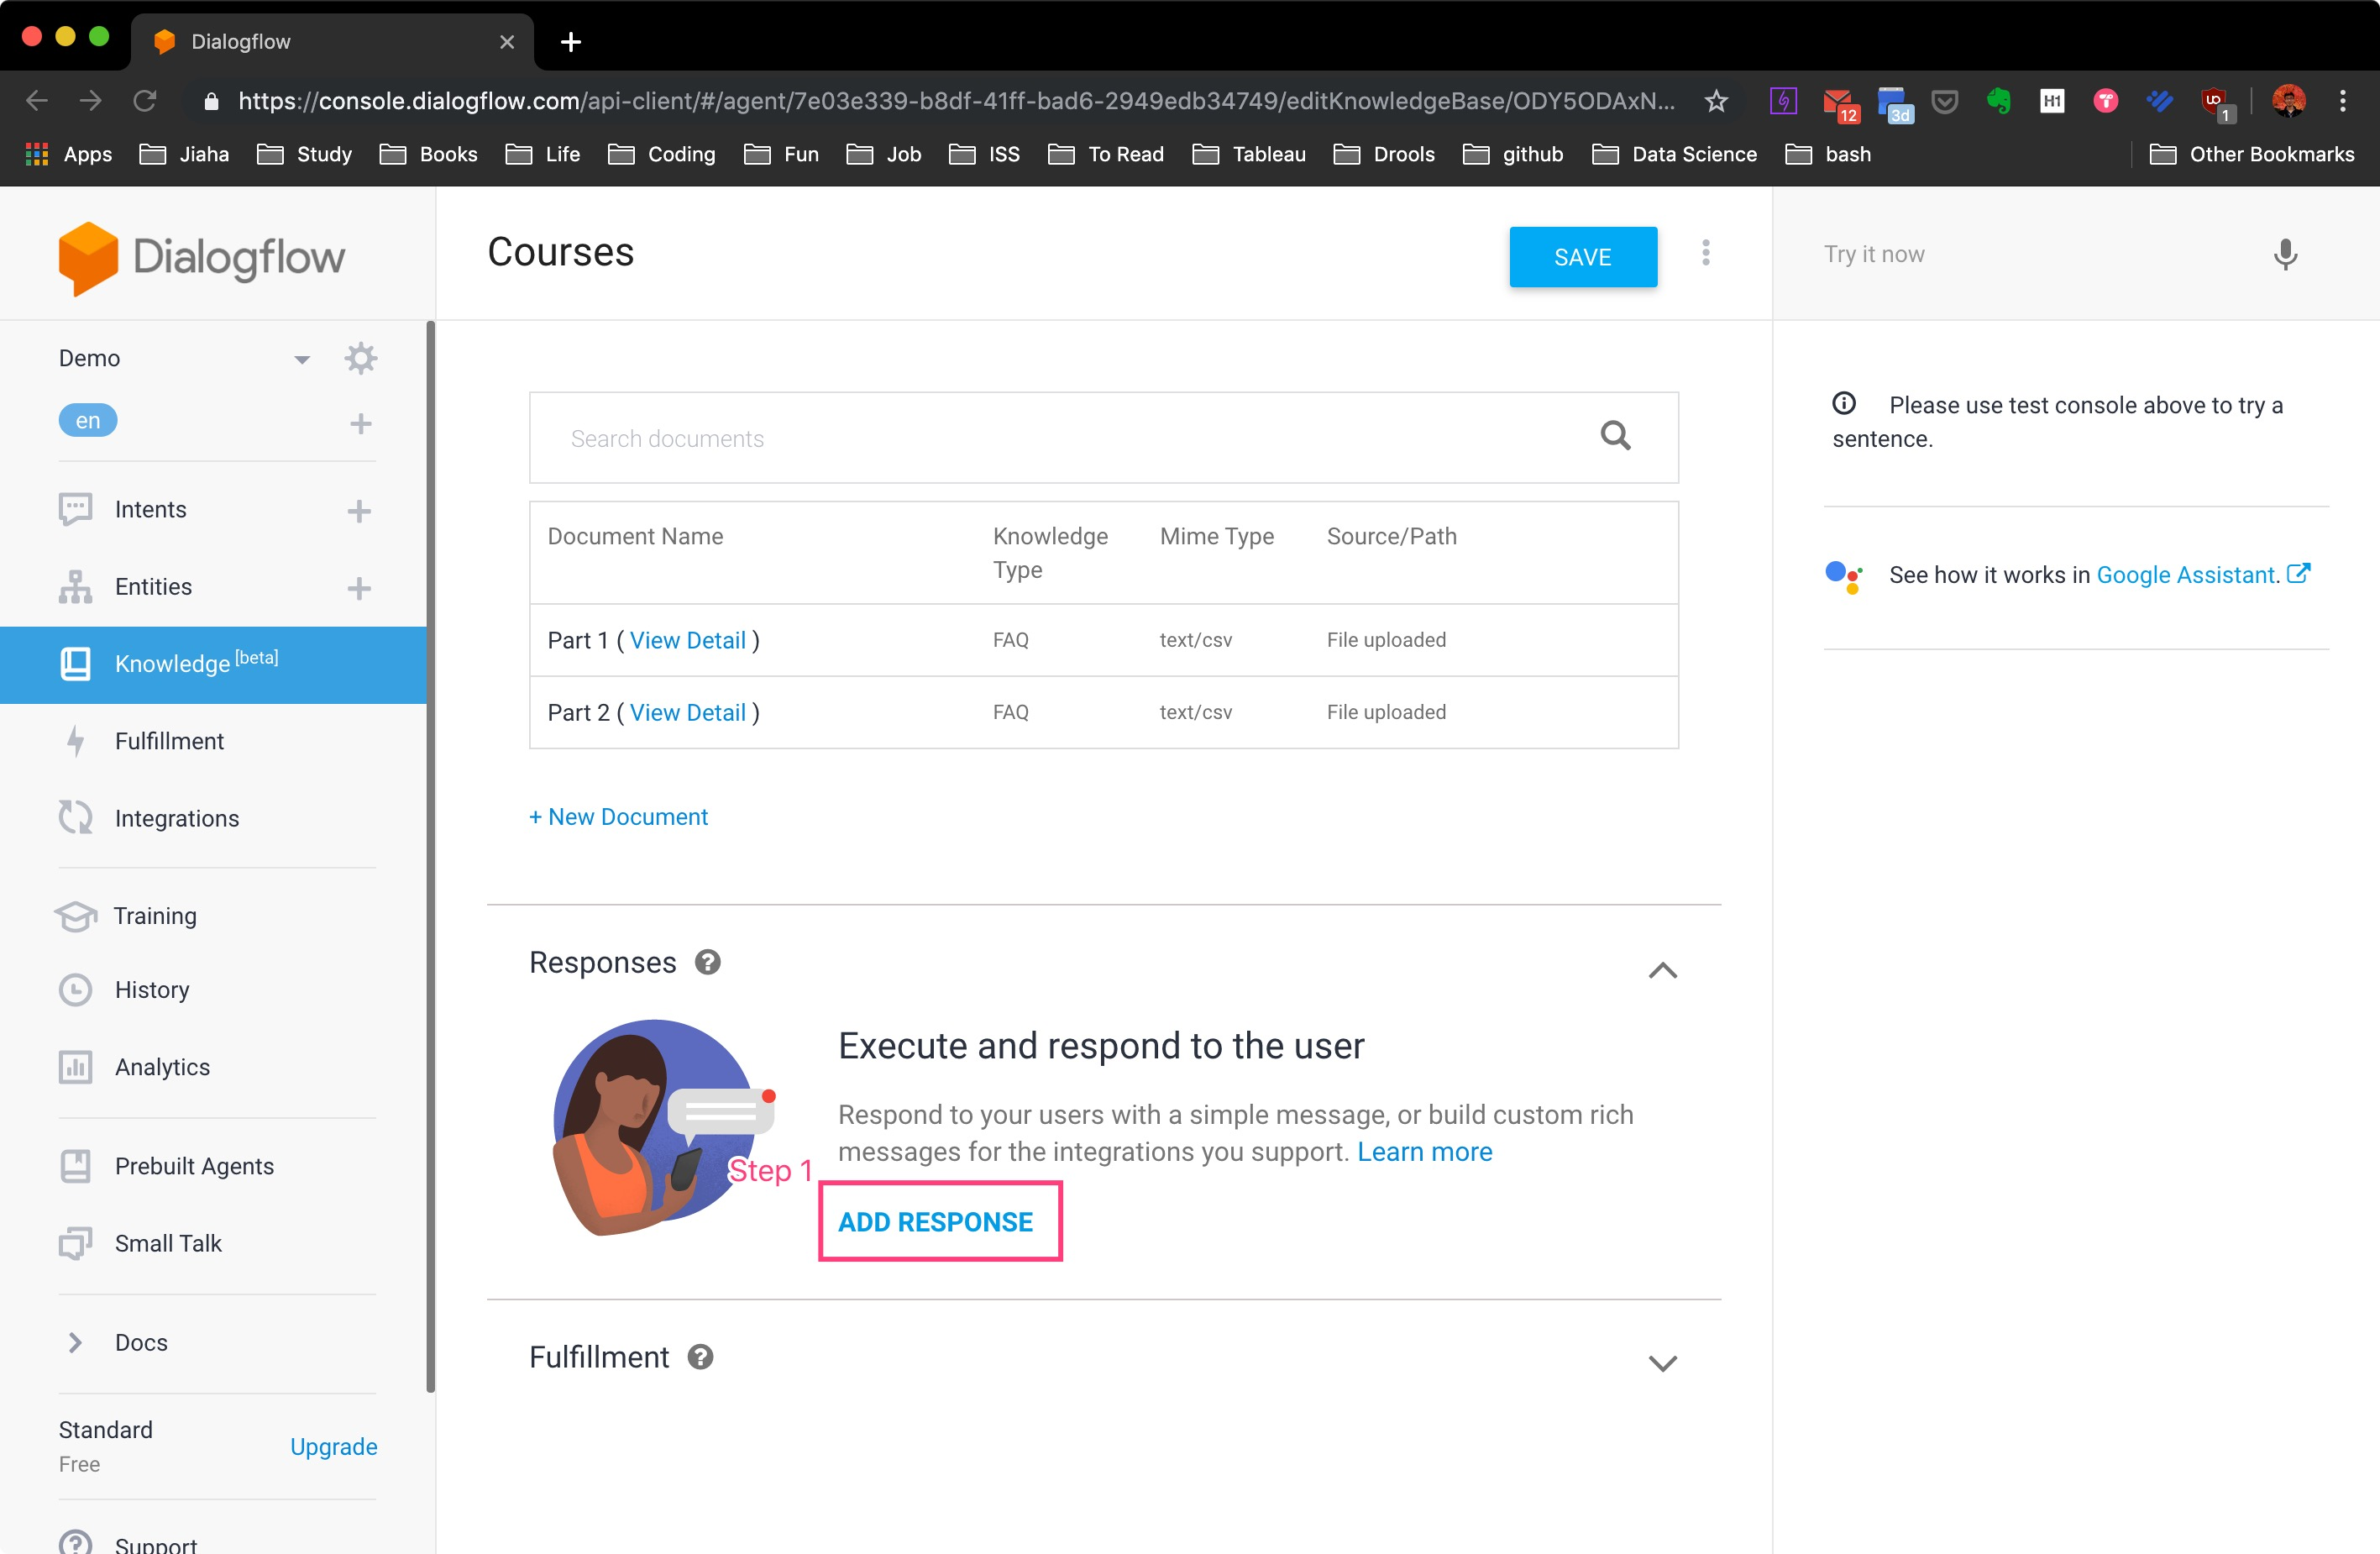
\includegraphics[width=\linewidth, frame]{img/manual_13.jpg}
	\end{figure}

	\item Click “SAVE” button
	\nopagebreak
	\begin{figure}[H]
		\centering
		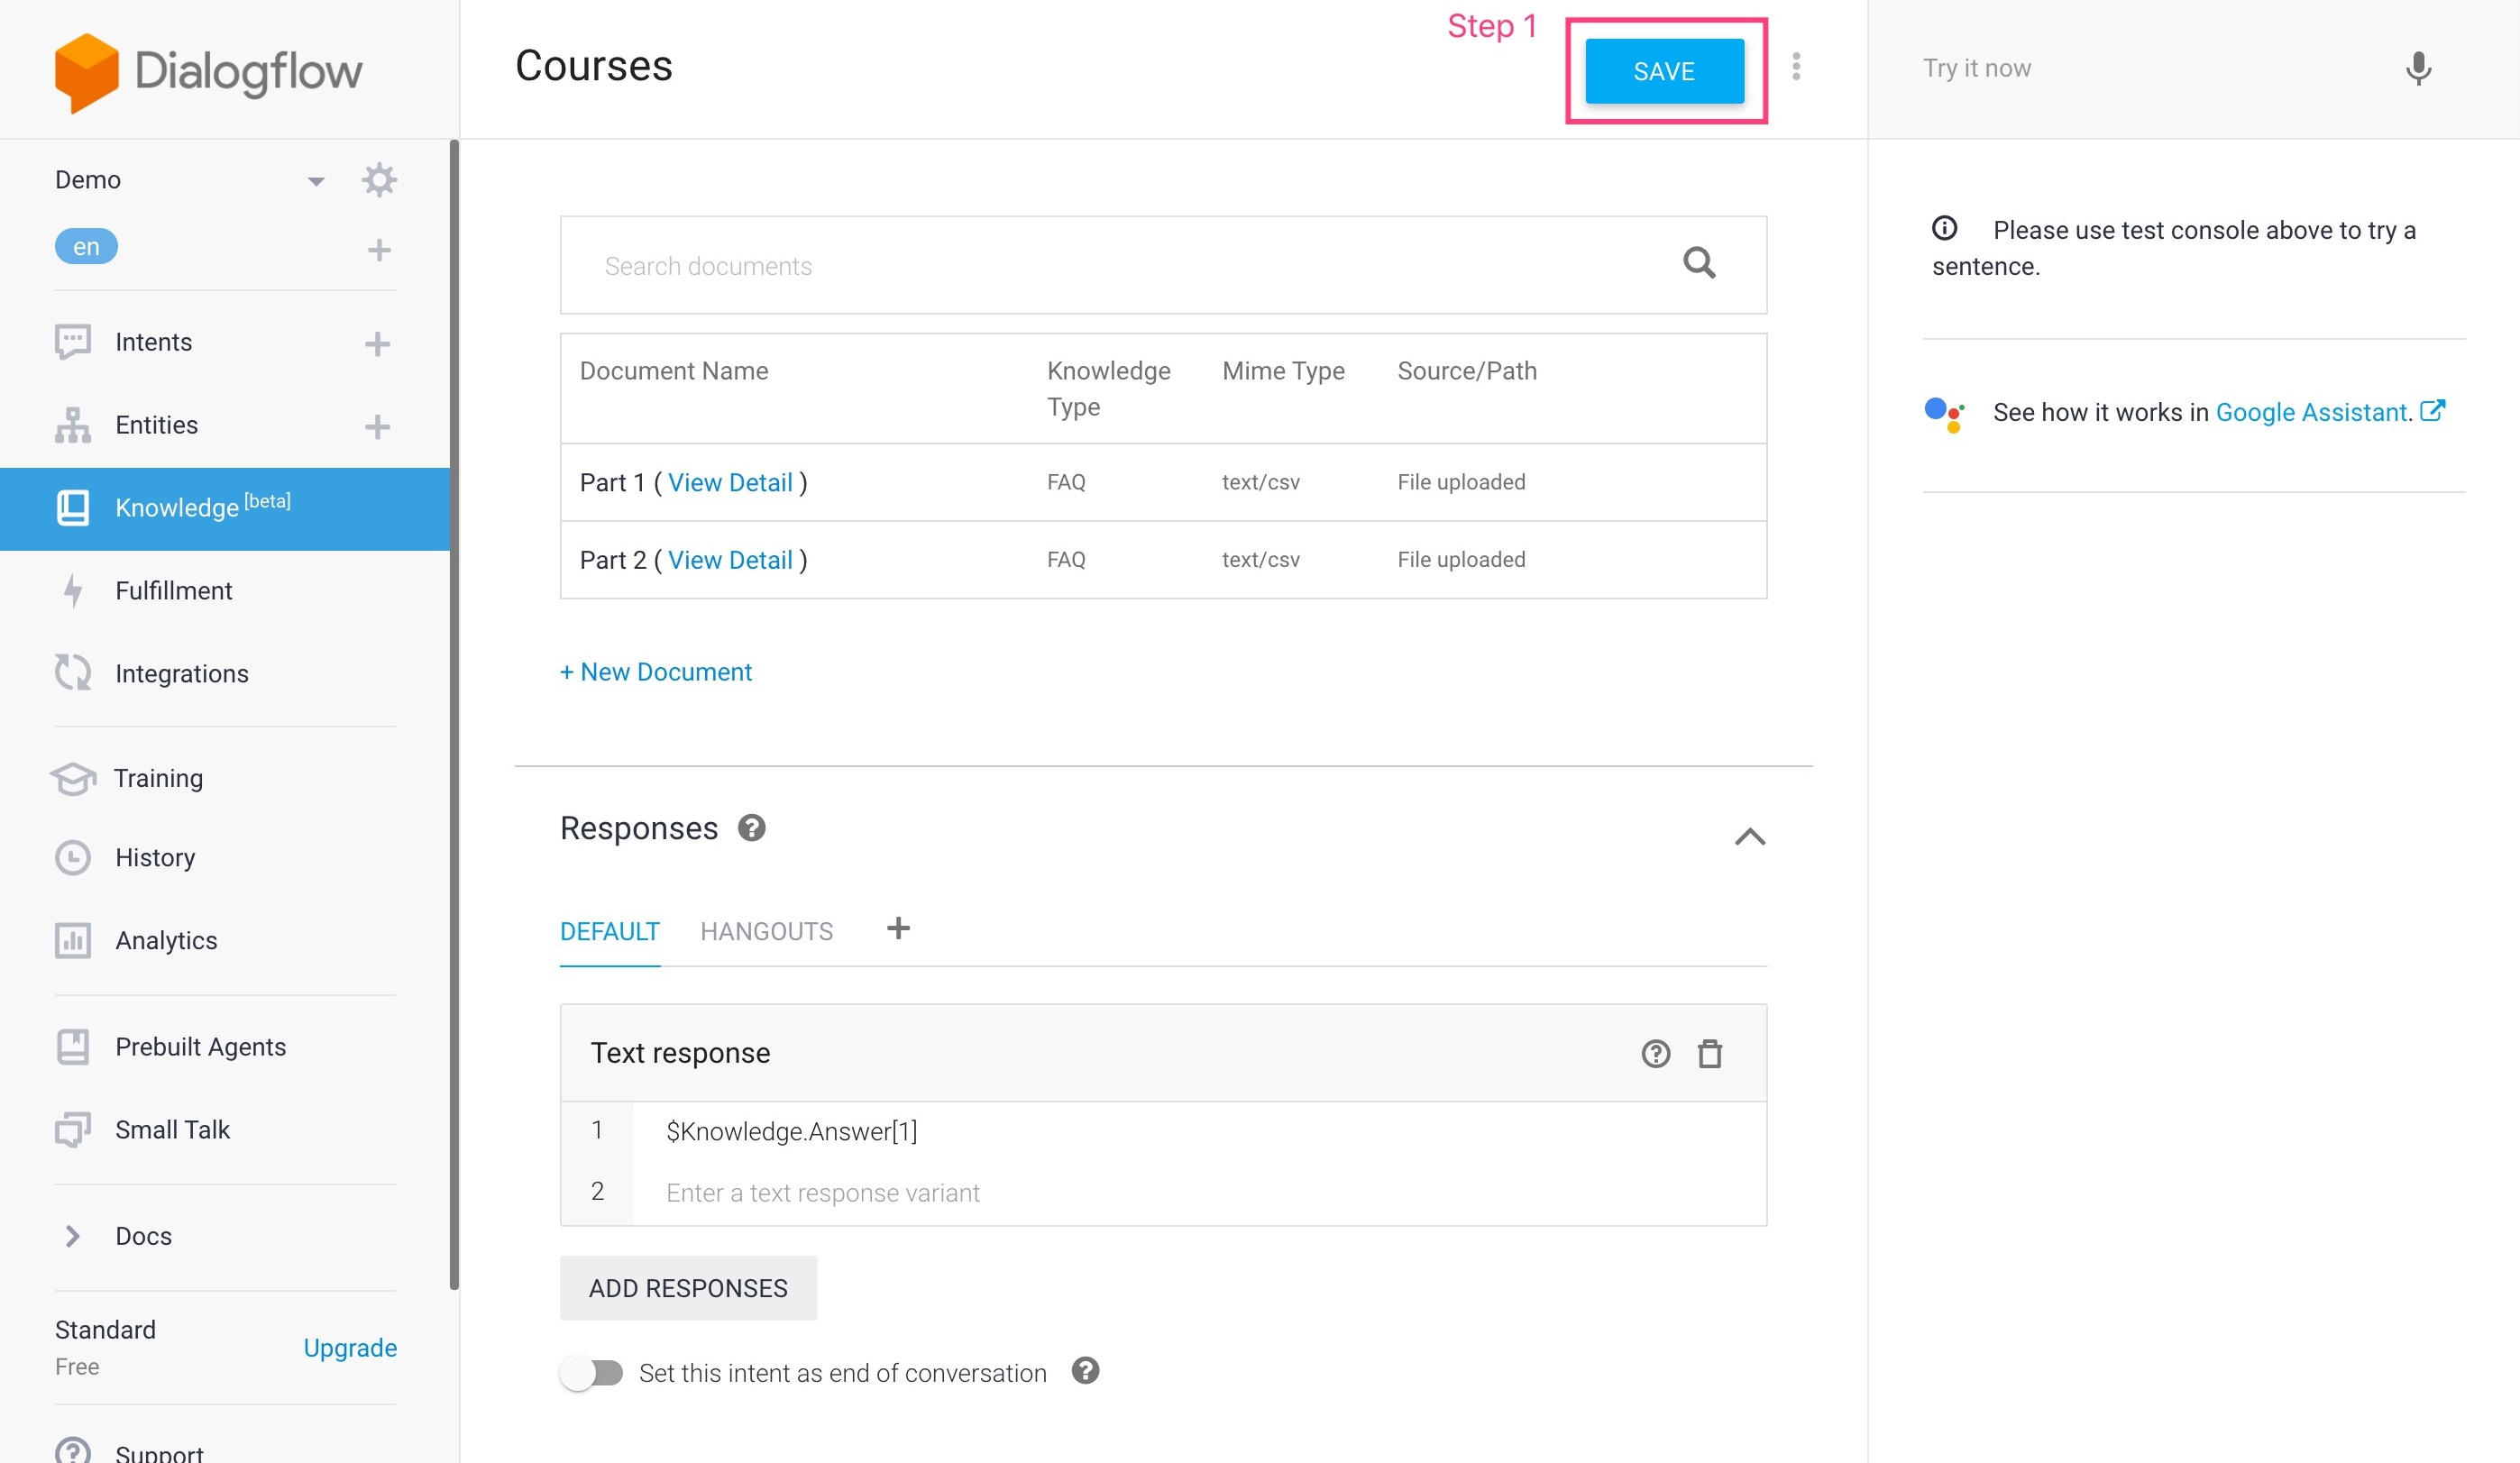
\includegraphics[width=\linewidth, frame]{img/manual_14.jpg}
	\end{figure}

\end{enumerate}
% section create_knowledge (end)

\section{Create Fulfilment} % (fold)
\label{sec:create_fulfilment}
	Click “Fulfillment” and enable “Inline Editor”, copy “IChat.js” and replace the content in “Index.js”. Then click “DEPLOY” button

	\begin{figure}[H]
		\centering
		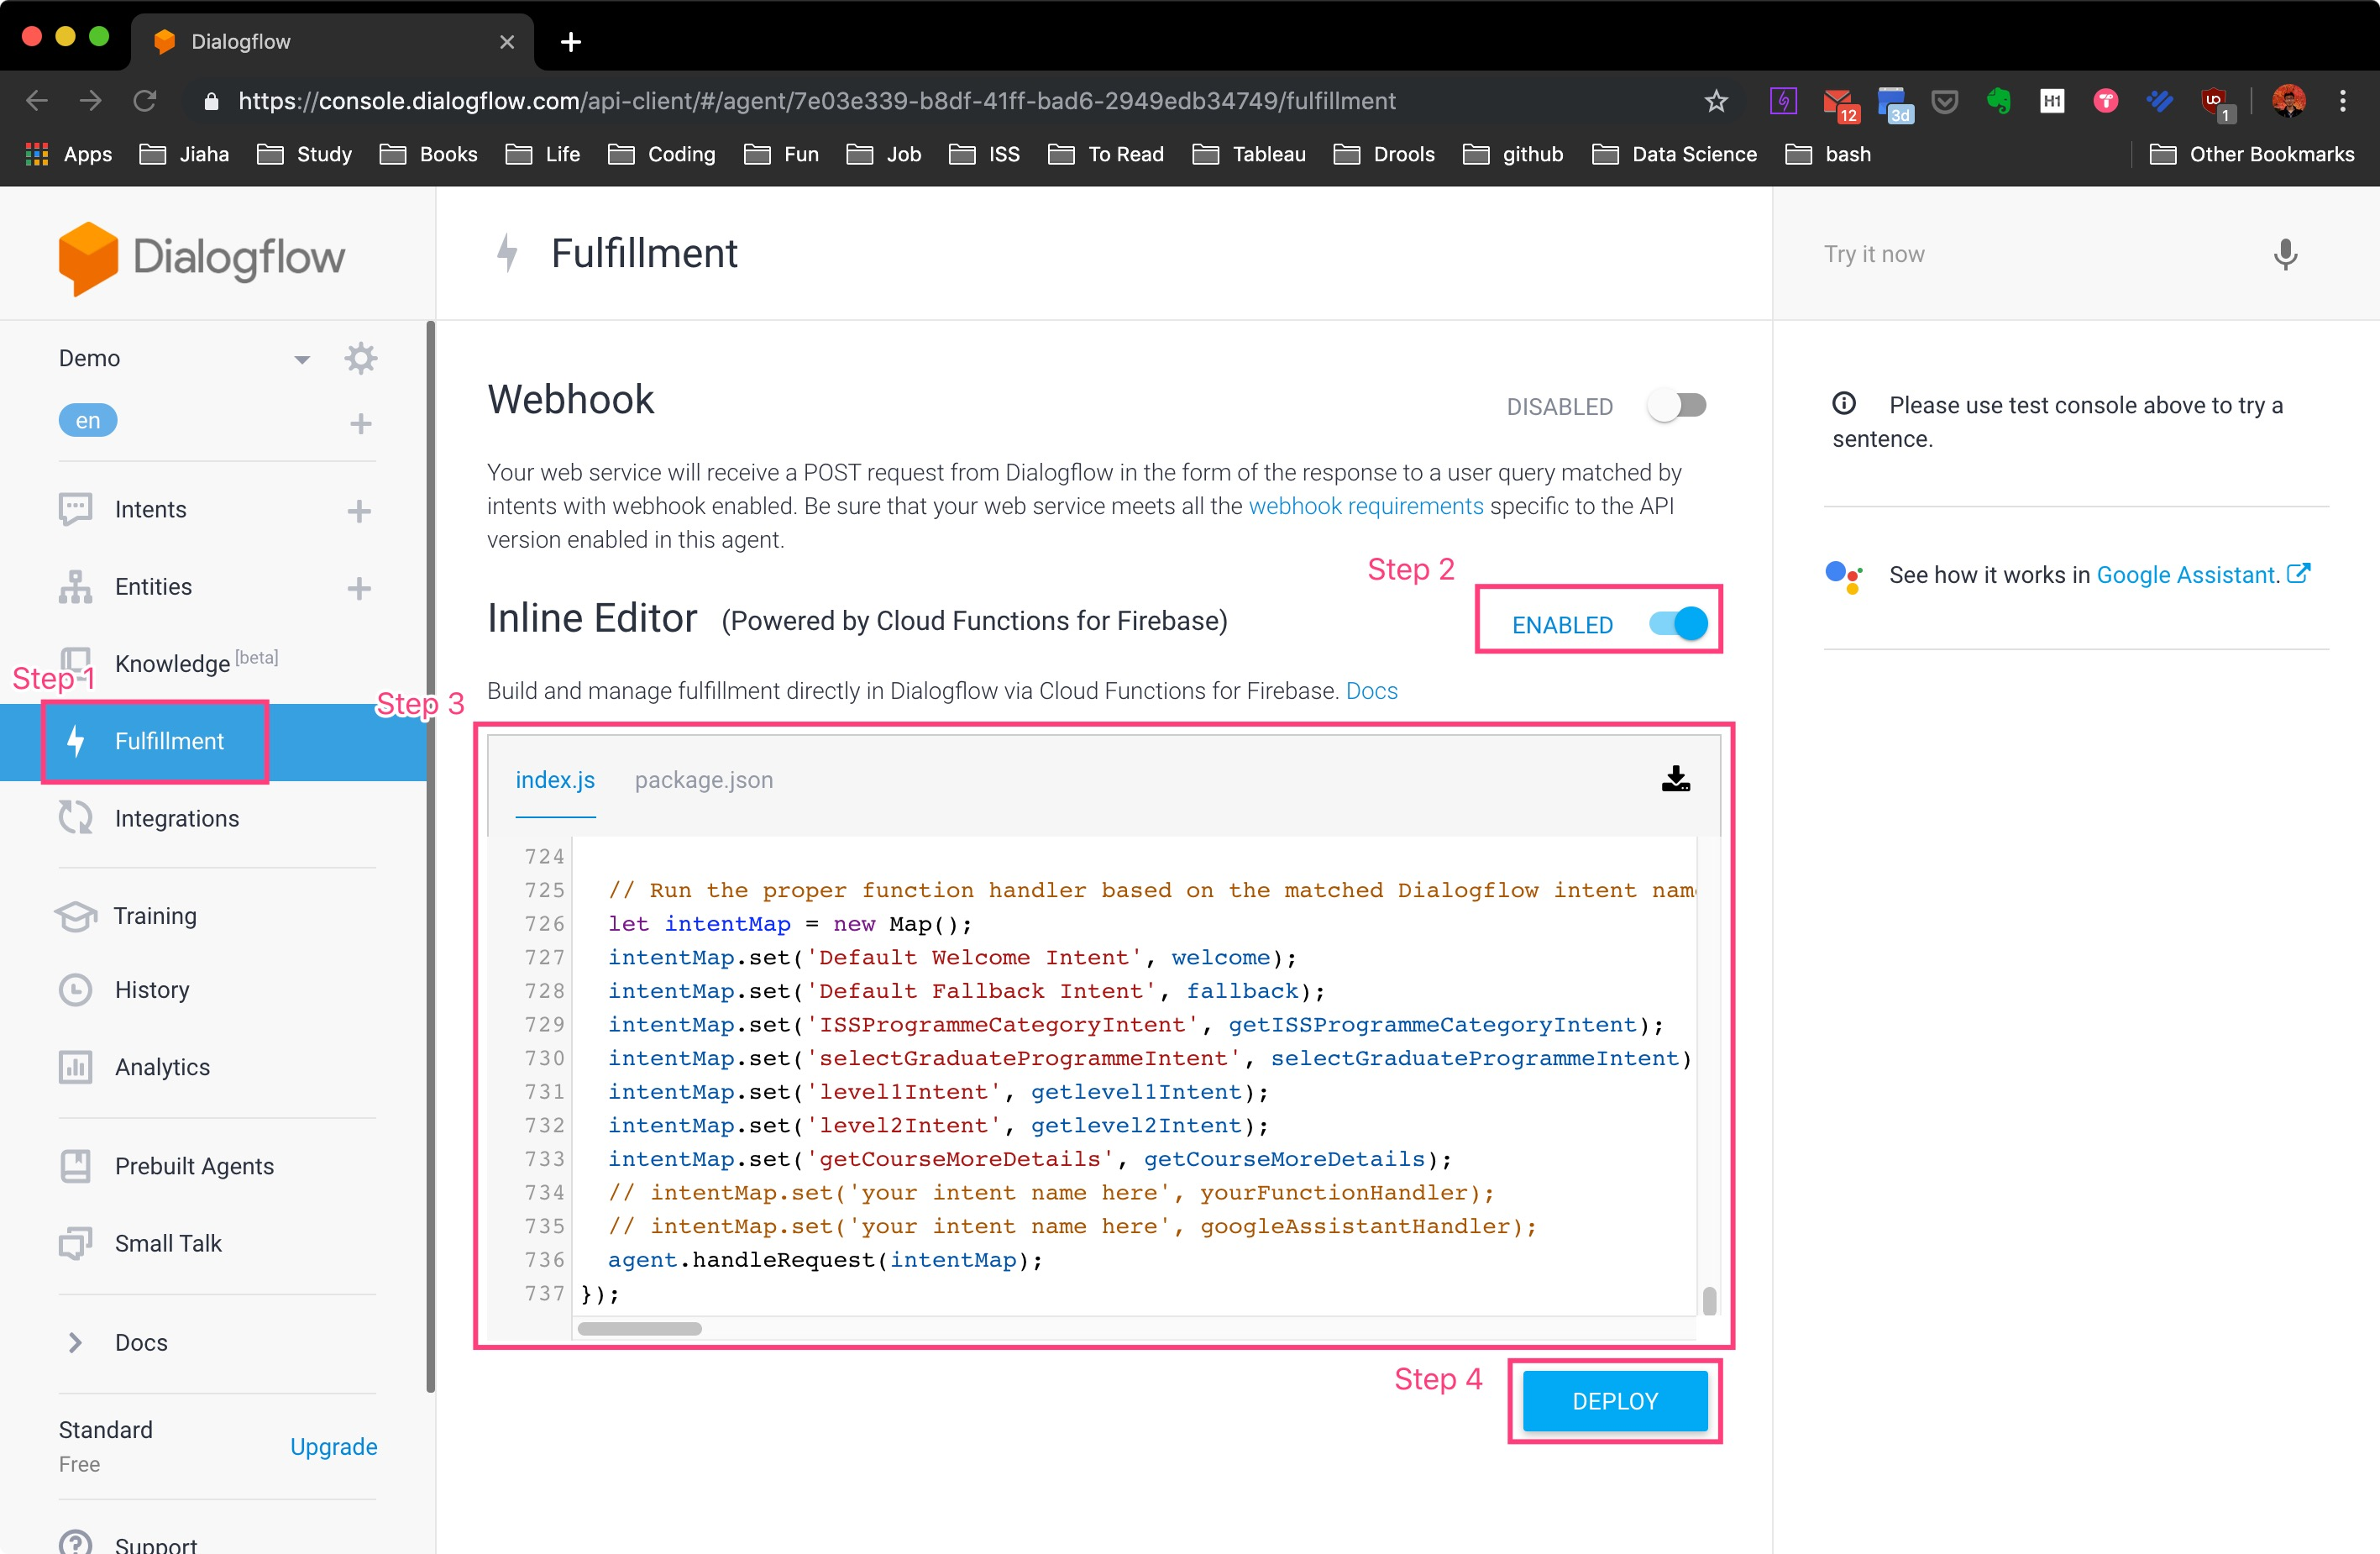
\includegraphics[width=\linewidth, frame]{img/manual_15.jpg}
	\end{figure}
% section create_fulfilment (end)

\section{Integration} % (fold)
\label{sec:integration}
	\begin{enumerate}
		\item Click “Integrations” and then enable “Slack”
		\nopagebreak
		\begin{figure}[H]
			\centering
			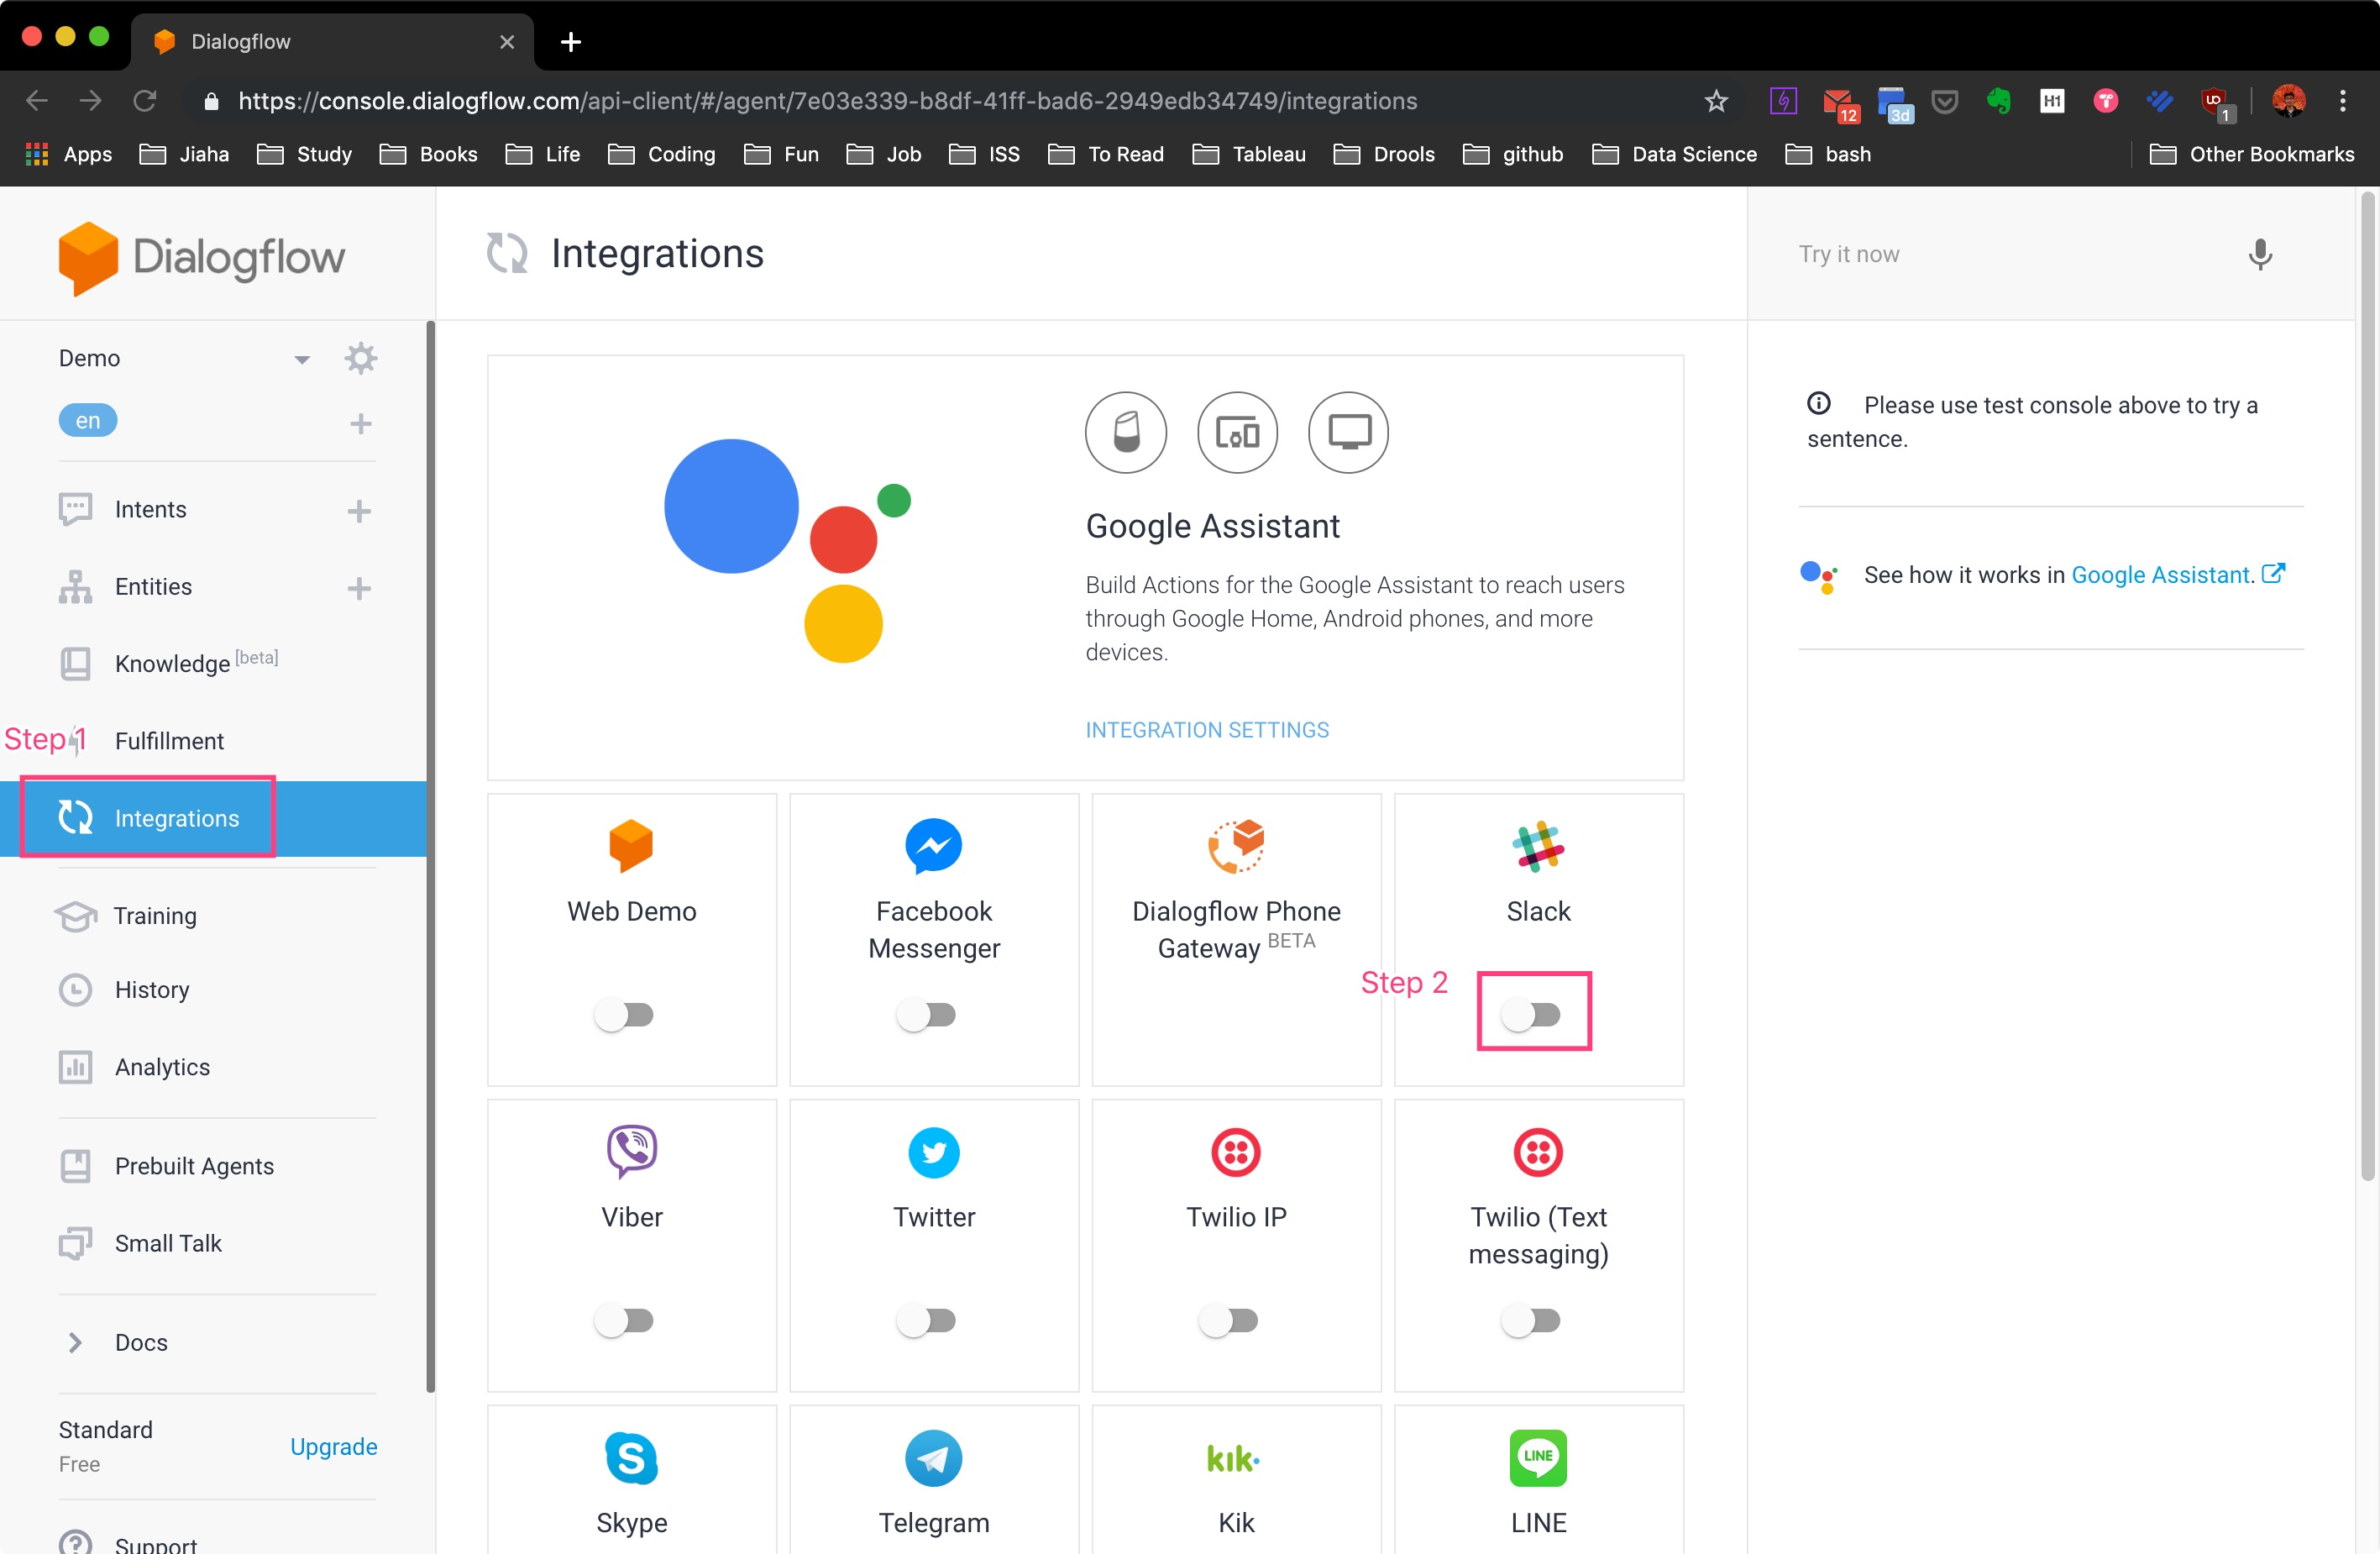
\includegraphics[width=\linewidth, frame]{img/manual_16.jpg}
		\end{figure}

		\item Follow the “Launch” to use, or click “TEST IN SLACK” with proper Slack set-up for testing

		\begin{figure}[H]
			\centering
			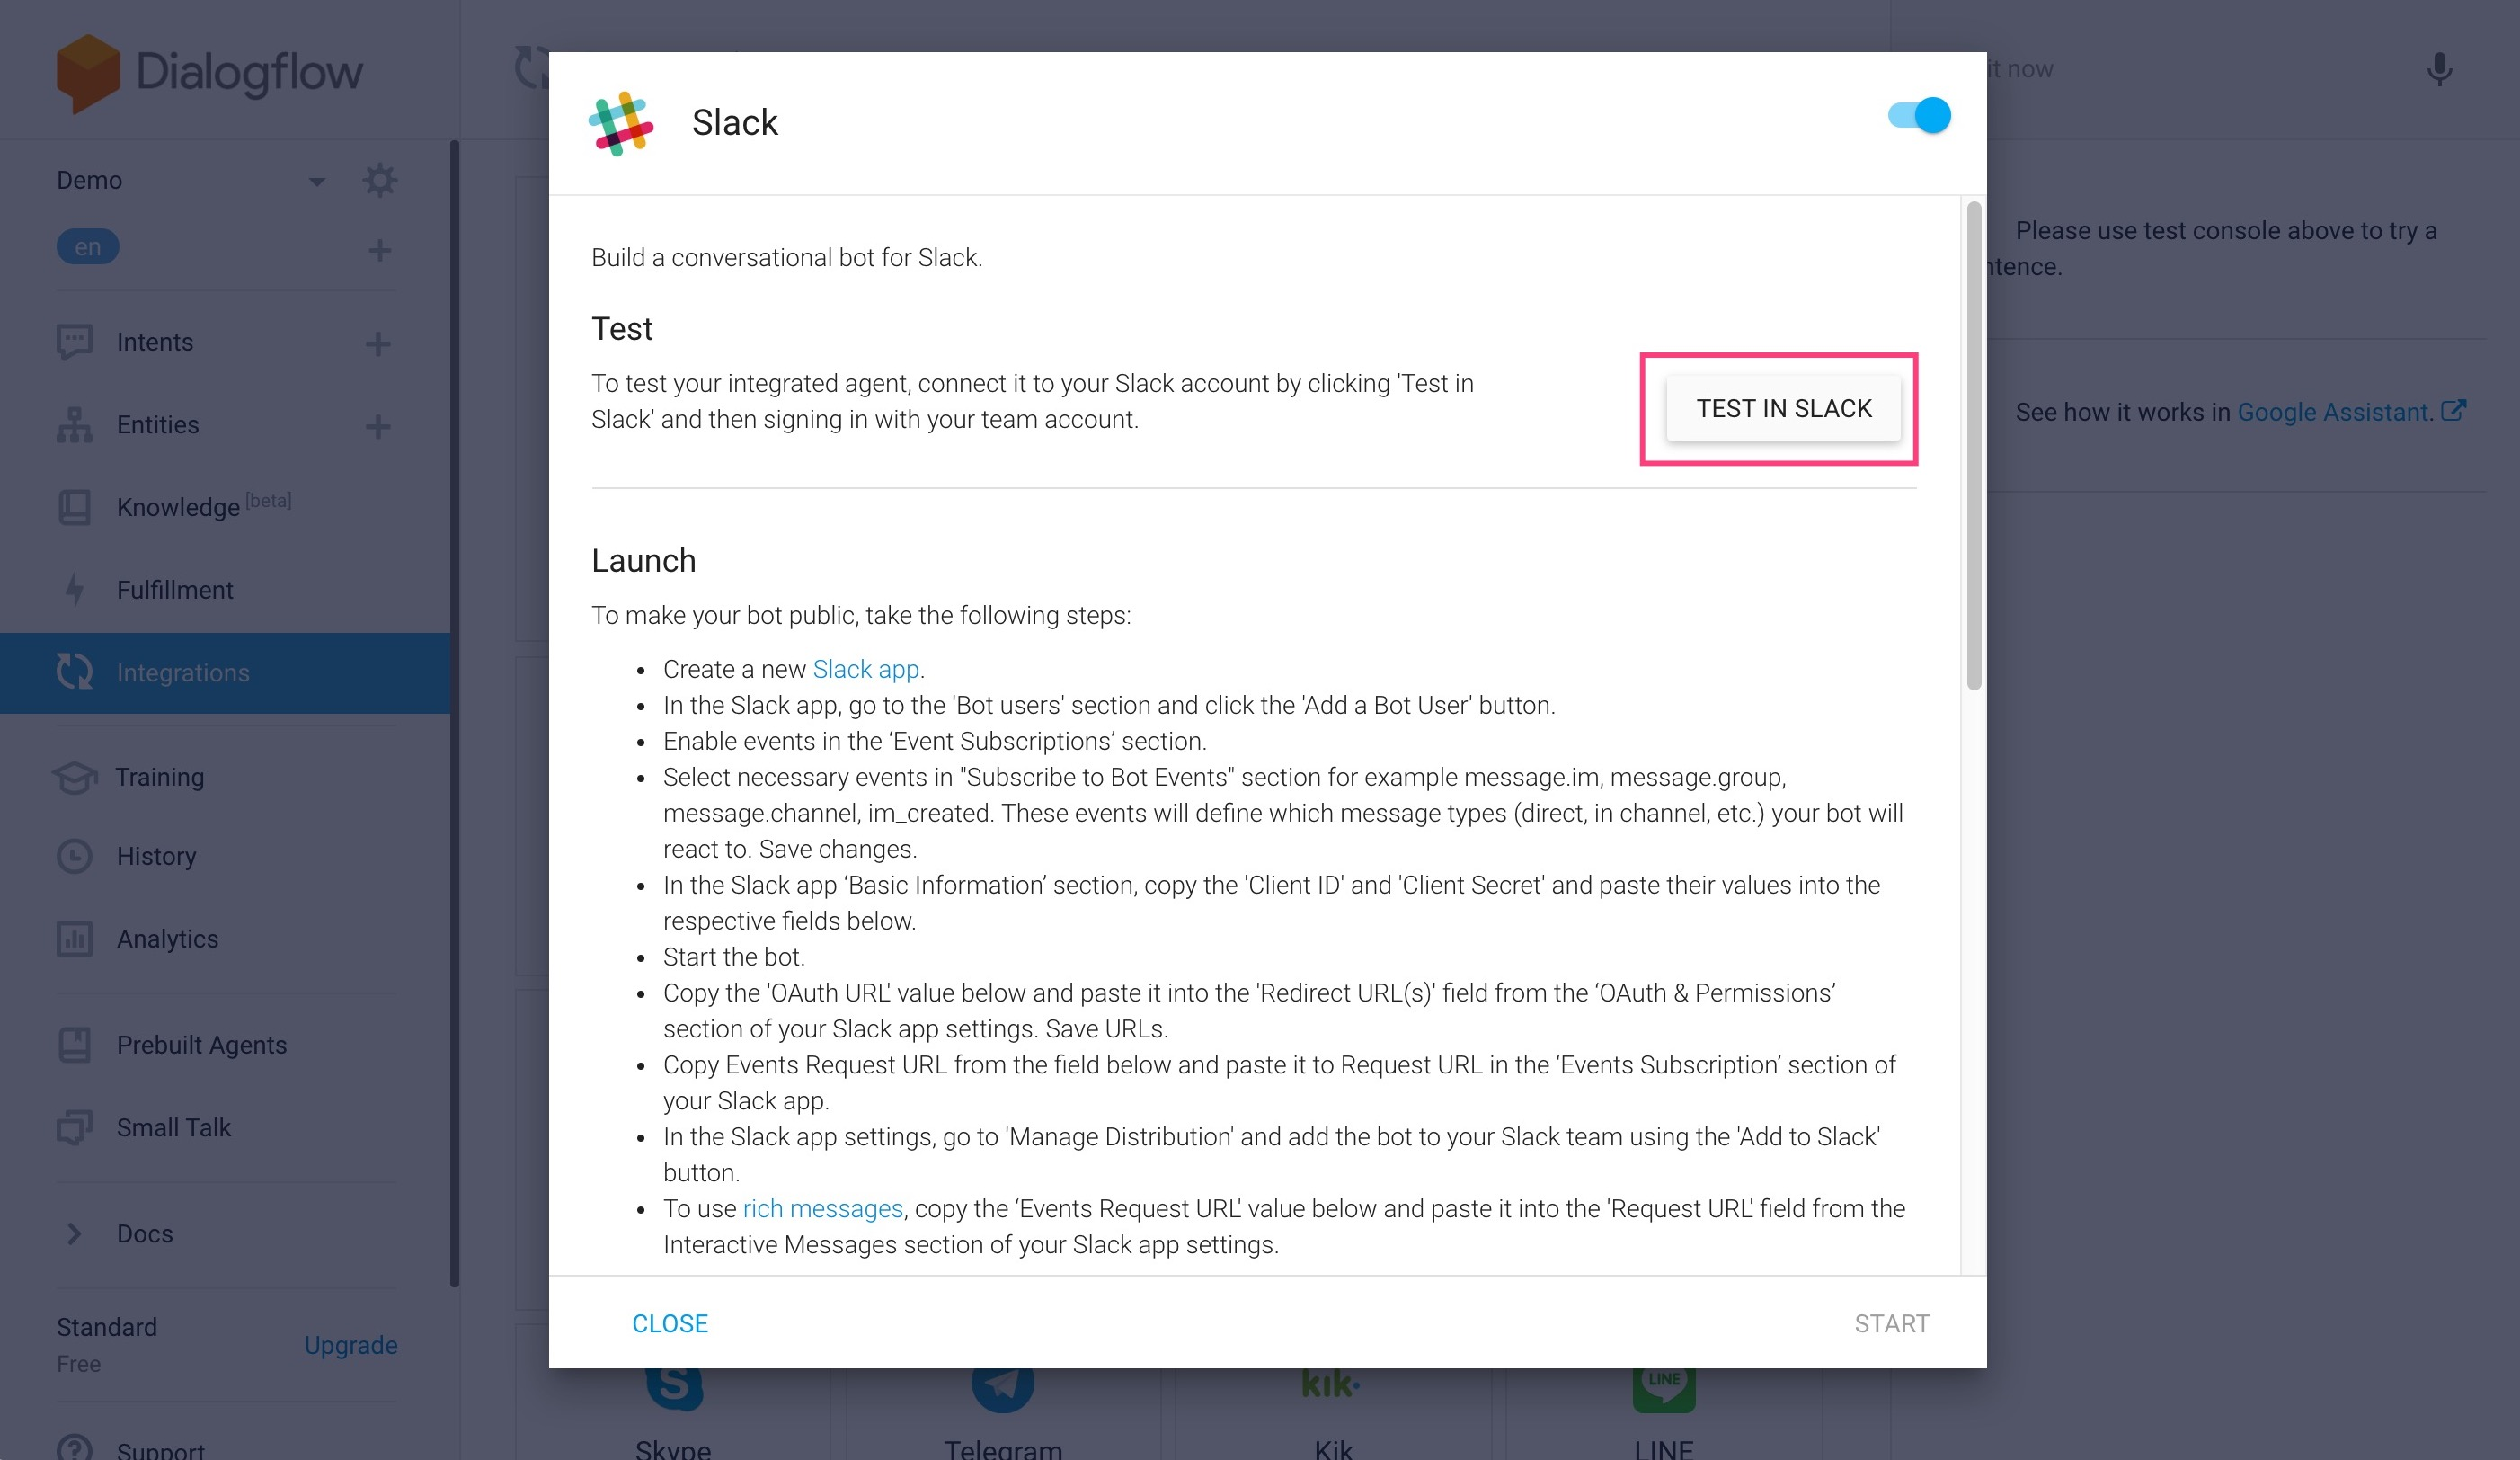
\includegraphics[width=\linewidth, frame]{img/manual_17.jpg}
		\end{figure}
	\end{enumerate}

% section integration (end)

\section{Test Demo} % (fold)
\label{sec:test}

	If Dialogflow is successfully integrated with Slack, you can say “hi” or other welcome words, and IChat will answer you enquiries.

	\begin{figure}[H]
		\centering
		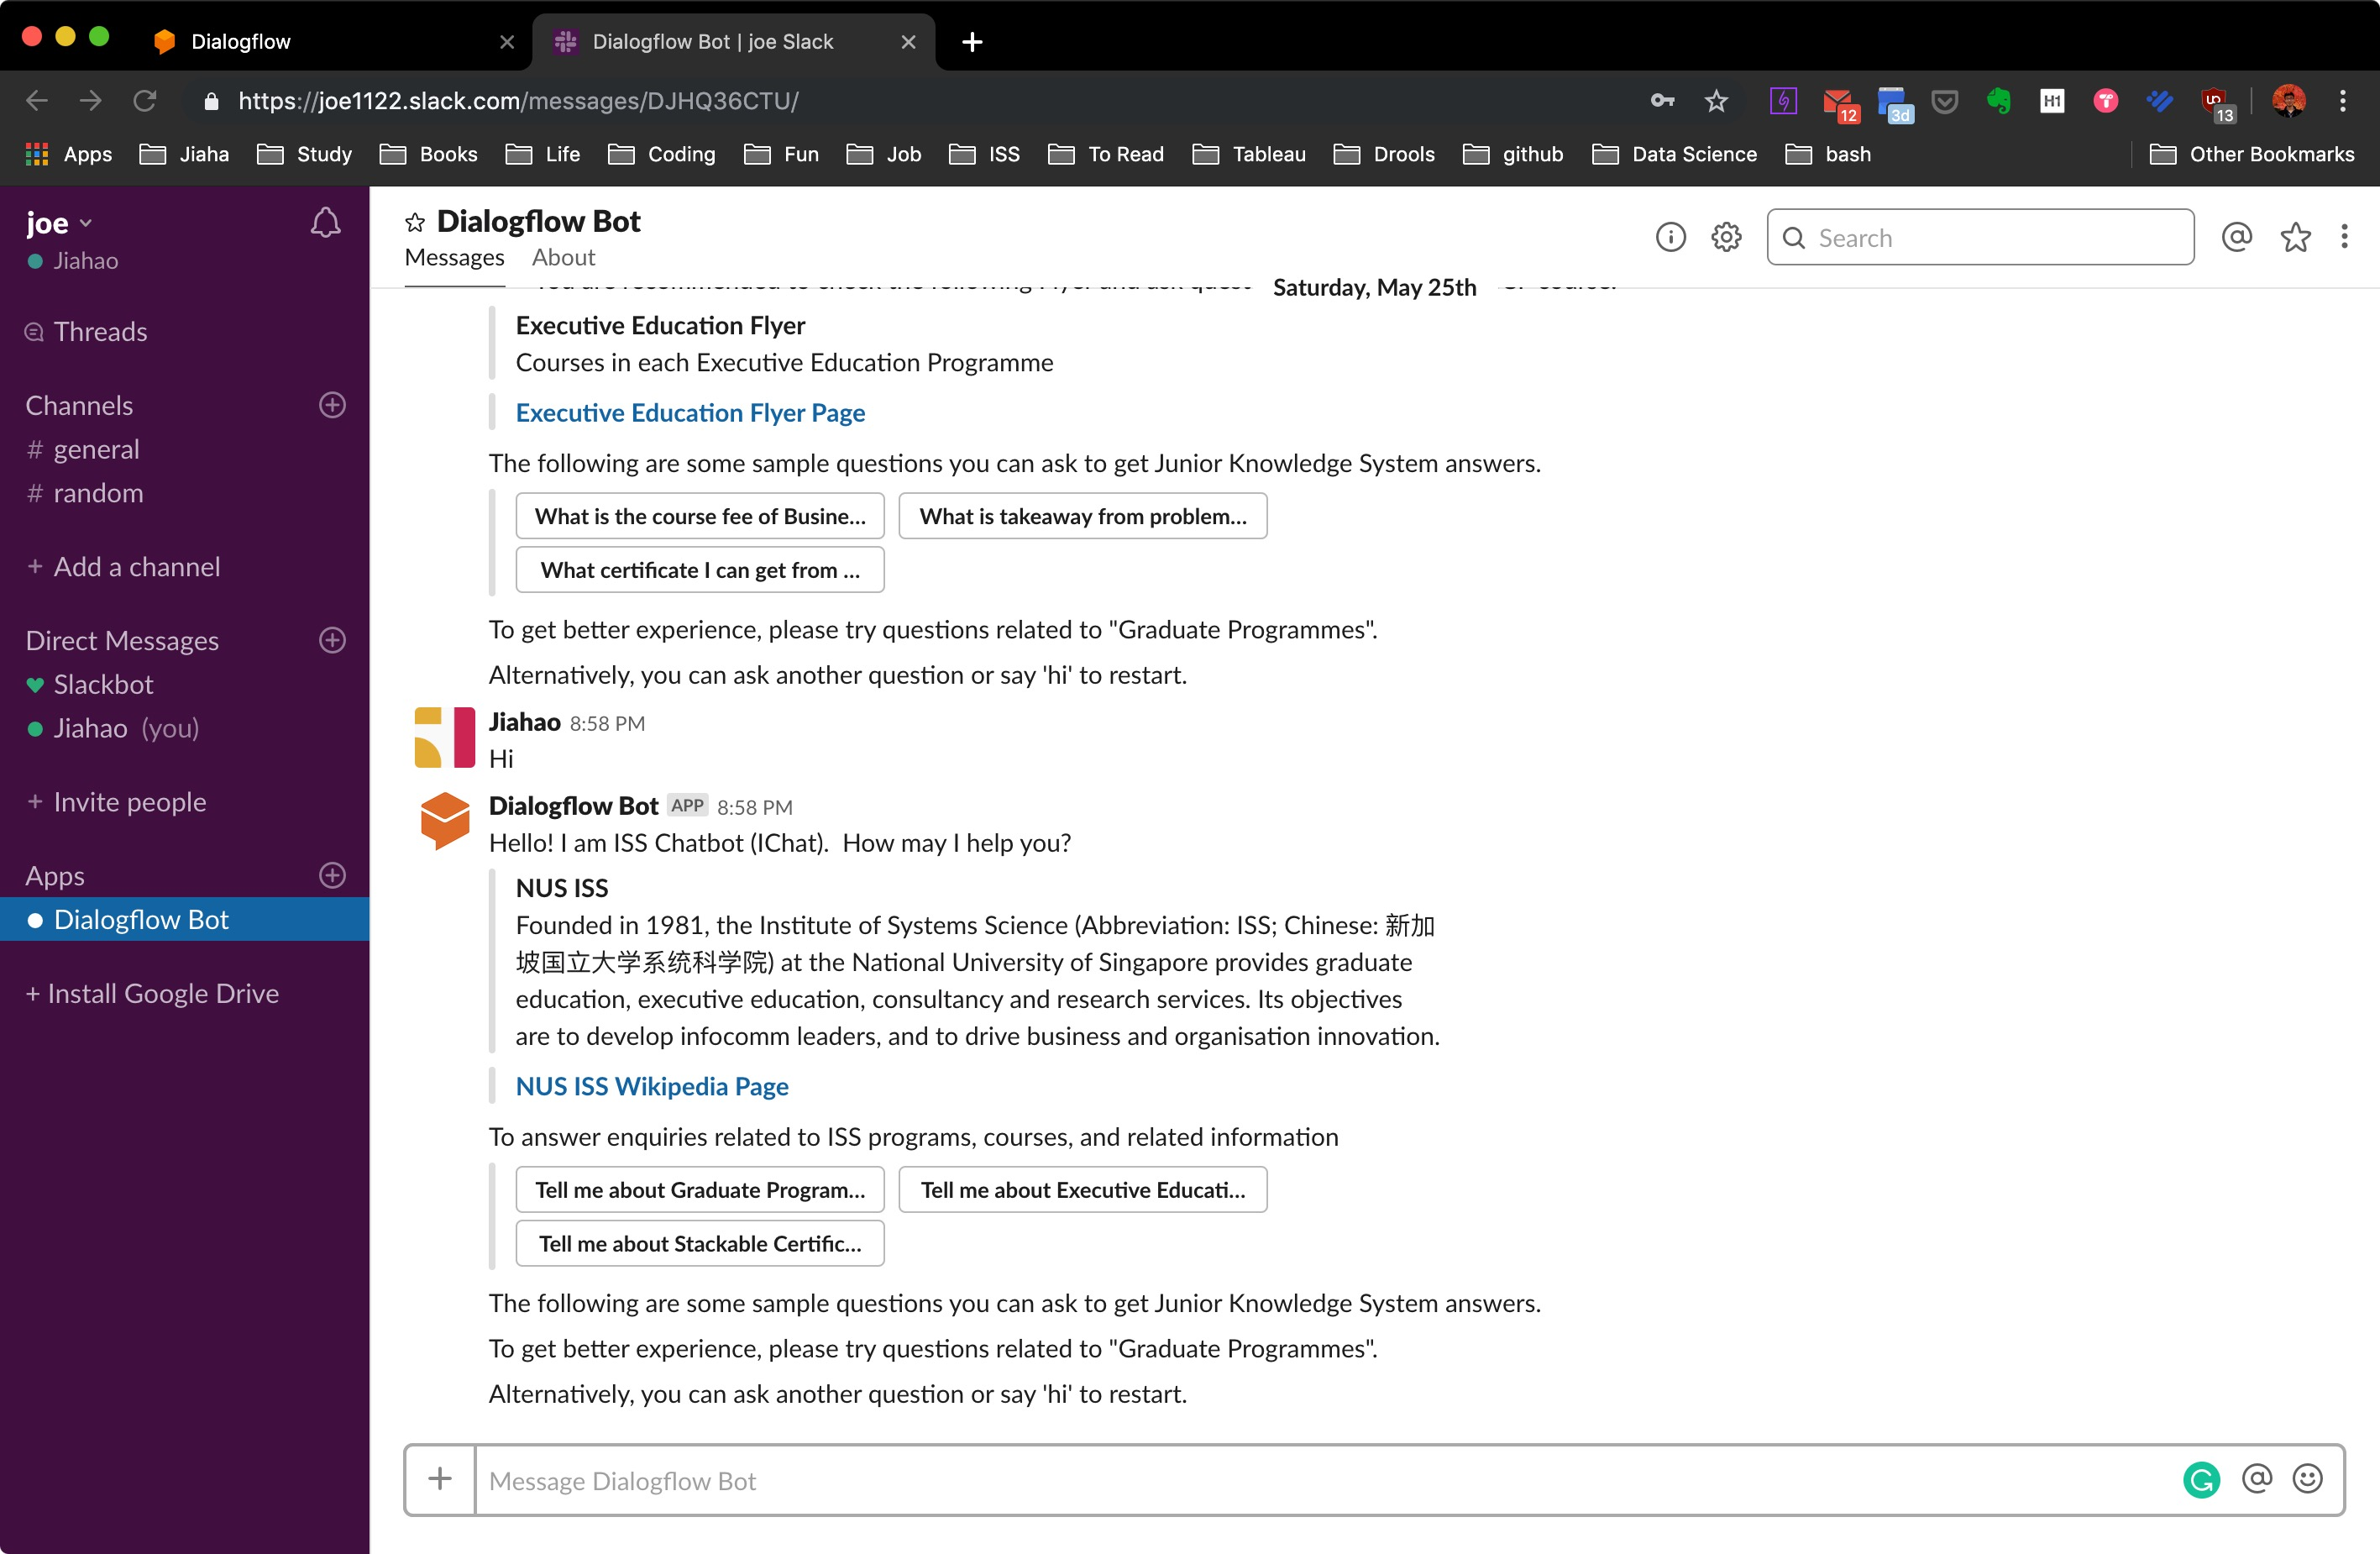
\includegraphics[width=\linewidth, frame]{img/manual_18.jpg}
	\end{figure}

	To easier test, the invite link is created for one of my demo.

	Here is the \href{https://join.slack.com/t/joe1122/shared_invite/enQtNjQxNTQ0MTY0Nzg1LTM3NDI3NGZjYWQzMjQ4YTJjMGIxZmQ4Y2VkMWYzNDAxOTQ0OTFlMmFjMzIzNDgyZjNkY2Q5YzQ2MjVlOTlmYWI}{\color{blue}{\underline{link}}}.

% section test (end)

\chapter{Test Result} % (fold)
\label{cha:test_result}

\begin{table}[h]
\centering
\resizebox{\textwidth}{!}{%
\begin{tabular}{|p{7cm}|p{5cm}|p{2cm}|p{2cm}|}
	\hline
	Can you give me an overview of Machine Reasoning? & Knowledge & 0.871 & \cellcolor[HTML]{9AFF99}Pass \\ \hline
	About Machine Reasoning & Knowledge & 0.671 & \cellcolor[HTML]{9AFF99}Pass \\ \hline
	What are the Machine Reasoning course pre-requsites? & Knowledge & 0.974 & \cellcolor[HTML]{9AFF99}Pass \\ \hline
	What are the Machine Reasoning course pre-requested knowledge? & Knowledge & 0.974 & \cellcolor[HTML]{9AFF99}Pass \\ \hline
	What are the Machine Reasoning course learning points? & Knowledge & 0.974 & \cellcolor[HTML]{9AFF99}Pass \\ \hline
	Learning result of Machine Reasoning & Knowledge & 0.587 & \cellcolor[HTML]{9AFF99}Pass \\ \hline
	What is the Machine Reasoning course key takeaway? & Knowledge & 0.974 & \cellcolor[HTML]{9AFF99}Pass \\ \hline
	Target Audience & Intent: Default Fallback Intent &  & \cellcolor[HTML]{FFCCC9}Fail \\ \hline
	Who should attend Machine Reasoning course? & Knowledge & 0.973 & \cellcolor[HTML]{9AFF99}Pass \\ \hline
	What will be covered in this Machine Reasoning course? & Knowledge & 0.976 & \cellcolor[HTML]{9AFF99}Pass \\ \hline
	What are the certs obtained from Machine Reasoning course? & Knowledge & 0.974 & \cellcolor[HTML]{9AFF99}Pass \\ \hline
	How much is Machine Reasoning? & Knowledge & 0.961 & \cellcolor[HTML]{9AFF99}Pass \\ \hline
	What are price for the Machine Reasoning? & Knowledge & 0.968 & \cellcolor[HTML]{9AFF99}Pass \\ \hline
	What are the Machine Reasoning course fees? & Knowledge & 0.974 & \cellcolor[HTML]{9AFF99}Pass \\ \hline
\end{tabular}%
}
\caption{FAQ Test}
\label{table:faq_test}
\end{table}

\begin{table}[h]
\centering
\resizebox{\textwidth}{!}{%
\begin{tabular}{|p{7cm}|p{5cm}|p{3cm}|}
	\hline
	\textbf{Test Question} & \textbf{Intent Returned} & \textbf{Final Test Case Result} \\ \hline
	Hi, tell me more about NUS ISS & Default Welcome Intent & \cellcolor[HTML]{9AFF99}Pass \\ \hline
	Graduate Programmes & ISSProgramCategoryIntent & \cellcolor[HTML]{9AFF99}Pass \\ \hline
	Overview of Master of Intelligence Systems & level1Intent & \cellcolor[HTML]{9AFF99}Pass \\ \hline
	Purpose & level2Intent & \cellcolor[HTML]{9AFF99}Pass \\ \hline
	Modules & level2Intent & \cellcolor[HTML]{9AFF99}Pass \\ \hline
	Price & level2Intent & \cellcolor[HTML]{9AFF99}Pass \\ \hline
	Application & level2Intent & \cellcolor[HTML]{9AFF99}Pass \\ \hline
	Career & level2Intent & \cellcolor[HTML]{9AFF99}Pass \\ \hline
	About Master of Intelligence Systems & level1Intent & \cellcolor[HTML]{9AFF99}Pass \\ \hline
	Learning Point & level2Intent & \cellcolor[HTML]{9AFF99}Pass \\ \hline
	Course & level2Intent & \cellcolor[HTML]{9AFF99}Pass \\ \hline
	Fees & level2Intent & \cellcolor[HTML]{9AFF99}Pass \\ \hline
	Application & level2Intent & \cellcolor[HTML]{9AFF99}Pass \\ \hline
	Furture Job & level2Intent & \cellcolor[HTML]{9AFF99}Pass \\ \hline
	Overview of Master of Intelligence Systems & level1Intent & \cellcolor[HTML]{9AFF99}Pass \\ \hline
	Purpose & level2Intent & \cellcolor[HTML]{9AFF99}Pass \\ \hline
	Courses & level2Intent & \cellcolor[HTML]{9AFF99}Pass \\ \hline
	School fee & level2Intent & \cellcolor[HTML]{9AFF99}Pass \\ \hline
	Admission & level2Intent & \cellcolor[HTML]{9AFF99}Pass \\ \hline
\end{tabular}%
}
\caption{Intent Test}
\label{table:intent_test}
\end{table}
% chapter test_result (end)

\chapter{Demo} % (fold)
\label{cha:demo}

	\section{Scenario 1} % (fold)
	\label{sec:scenario_1}
		A future student wants to check some information about \textbf{Master of Technology in Intelligent Systems}, which is under \textbf{Graduate Programme}. This student wants to know when the next intake time and how long will the programme last. In this scenario, the user only need to click suggestion button to get answers.

		\begin{figure}[H]
			\centering
			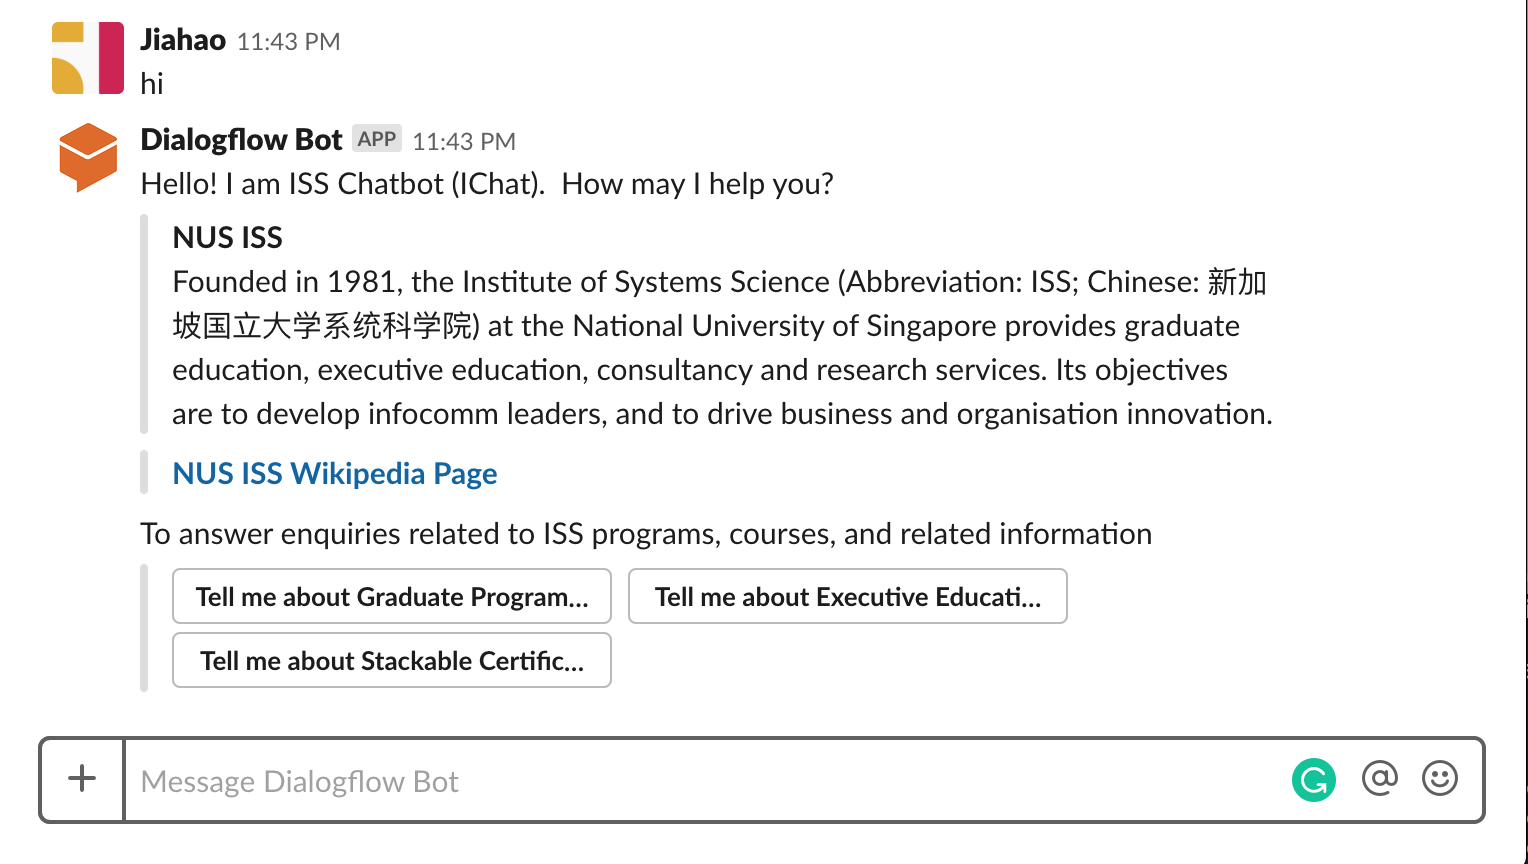
\includegraphics[width=\linewidth, frame]{img/scenario_1.png}
		\end{figure}

		\begin{figure}[H]
			\centering
			
\includegraphics[width=\linewidth, frame]{img/scenario_2.png}
		\end{figure}

		\begin{figure}[H]
			\centering
			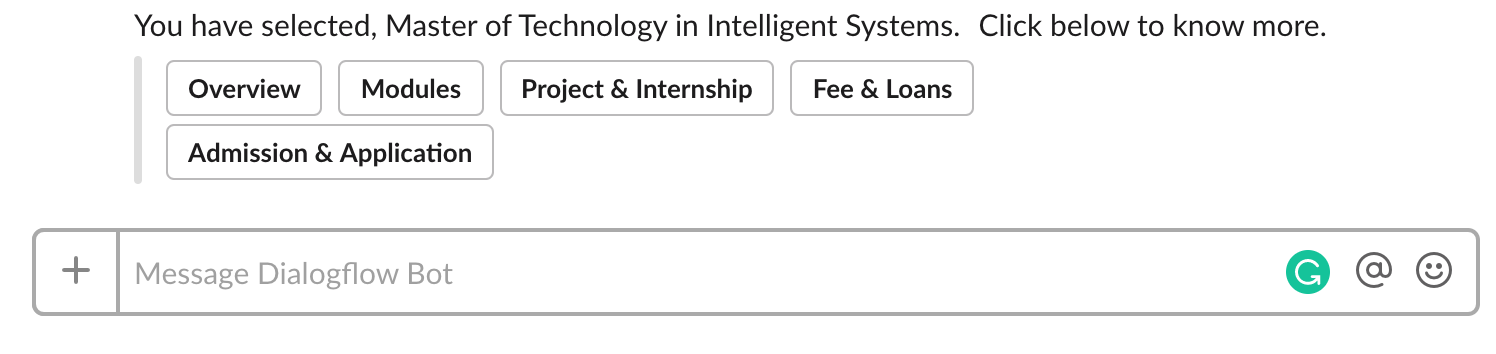
\includegraphics[width=\linewidth, frame]{img/scenario_3.png}
		\end{figure}

		\begin{figure}[H]
			\centering
			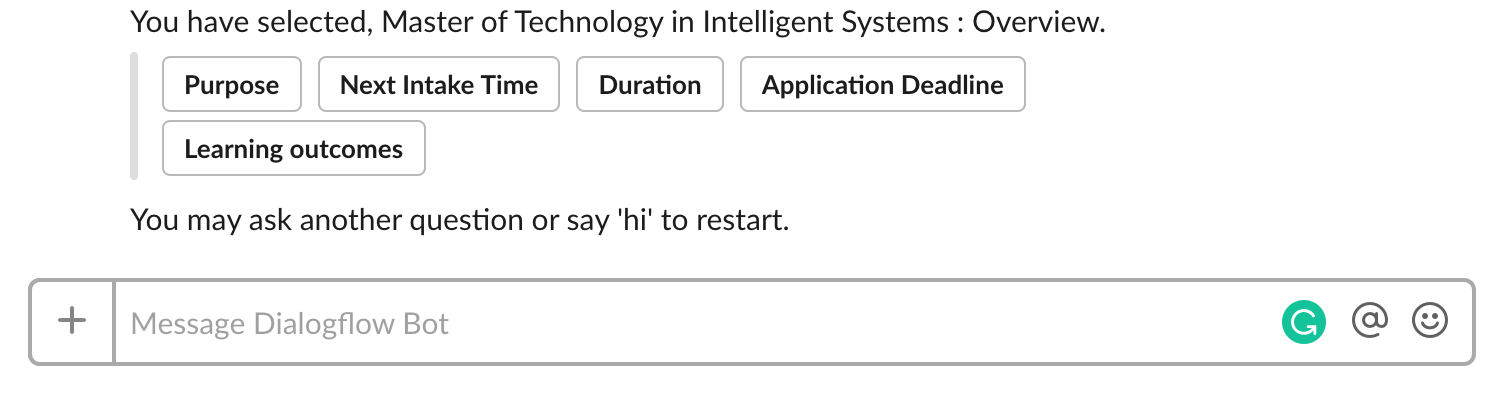
\includegraphics[width=\linewidth, frame]{img/scenario_4.png}
		\end{figure}

		\begin{figure}[H]
			\centering
			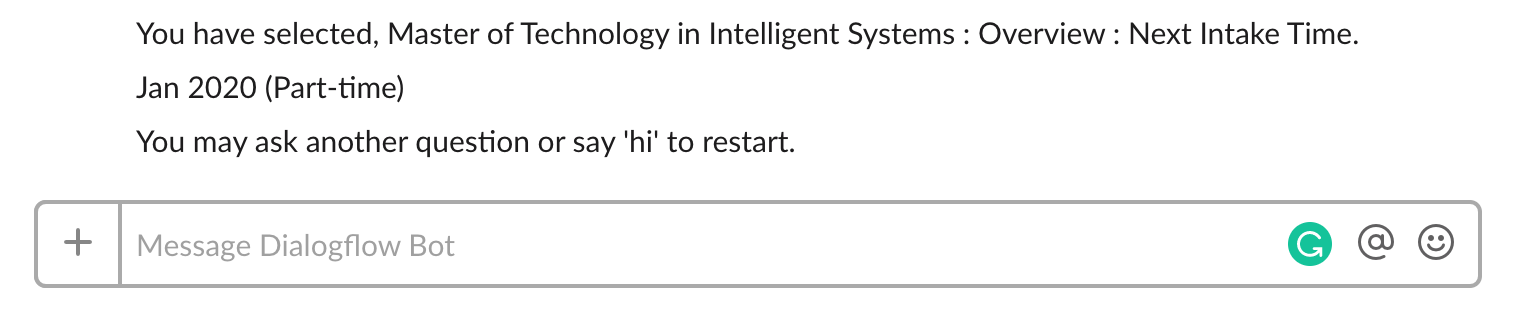
\includegraphics[width=\linewidth, frame]{img/scenario_5.png}
		\end{figure}

		\begin{figure}[H]
			\centering
			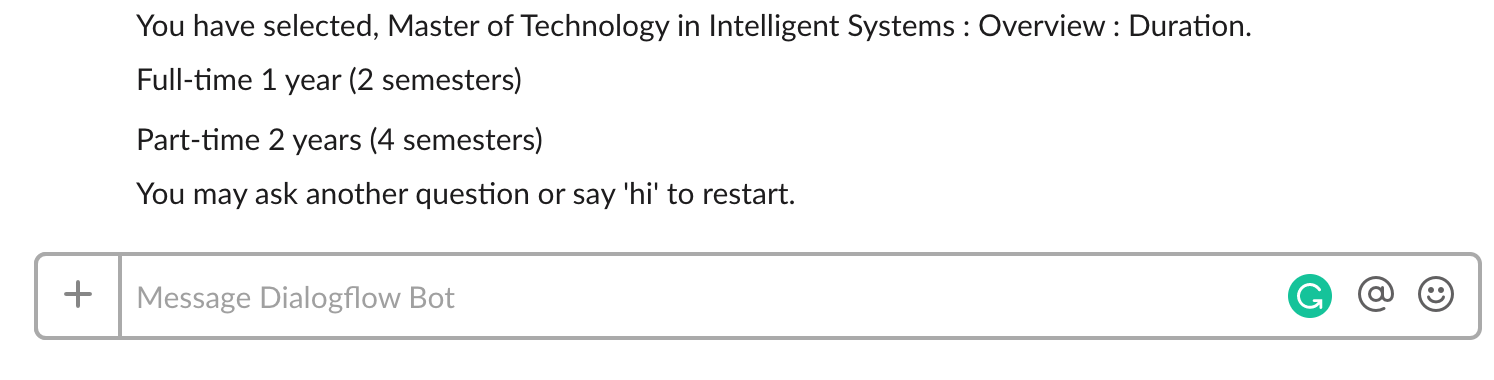
\includegraphics[width=\linewidth, frame]{img/scenario_6.png}
		\end{figure}
	% section scenario_1 (end)

	\section{Scenario 2} % (fold)
	\label{sec:scenario_2}
		An employee wants to learn more about \textbf{Machine Reasoning} course in \textbf{Executive Education Programmes}. The user needs to input questions related to the course in this scenario.

		\begin{figure}[H]
			\centering
			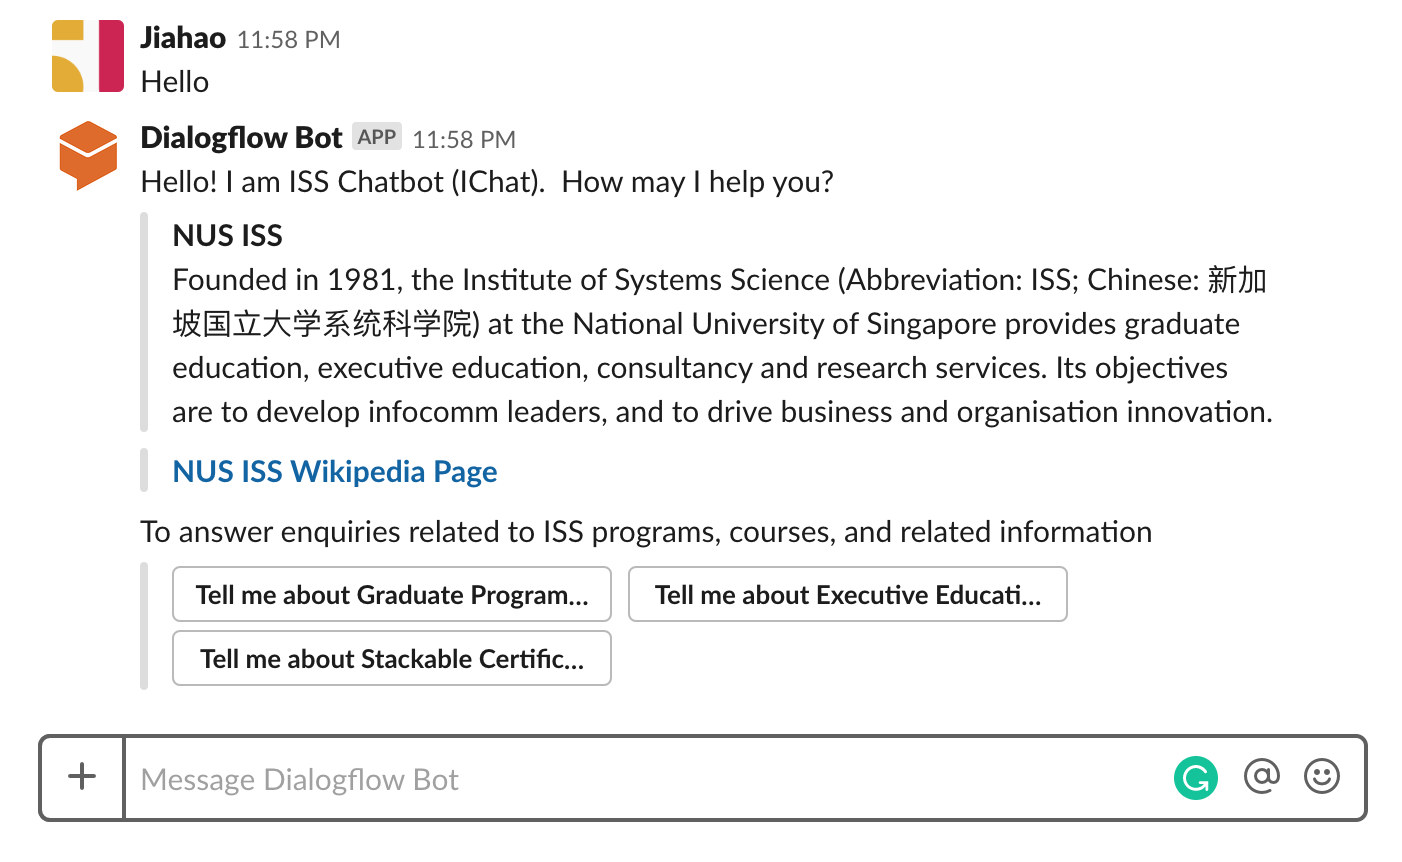
\includegraphics[width=\linewidth, frame]{img/scenario_2_1.png}
		\end{figure}

		\begin{figure}[H]
			\centering
			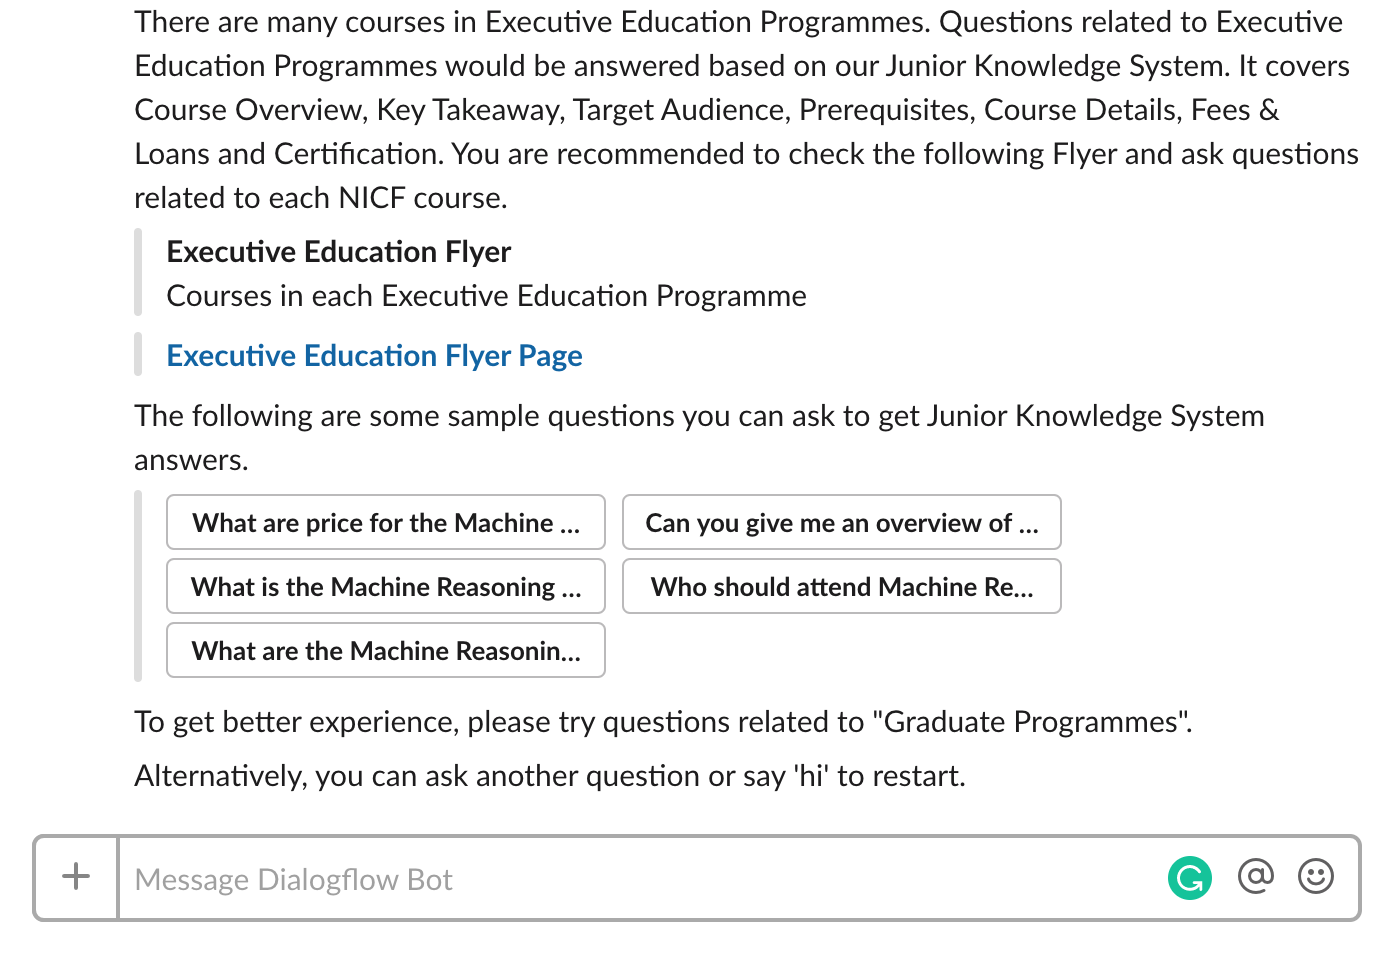
\includegraphics[width=\linewidth, frame]{img/scenario_2_2.png}
		\end{figure}

		\begin{figure}[H]
			\centering
			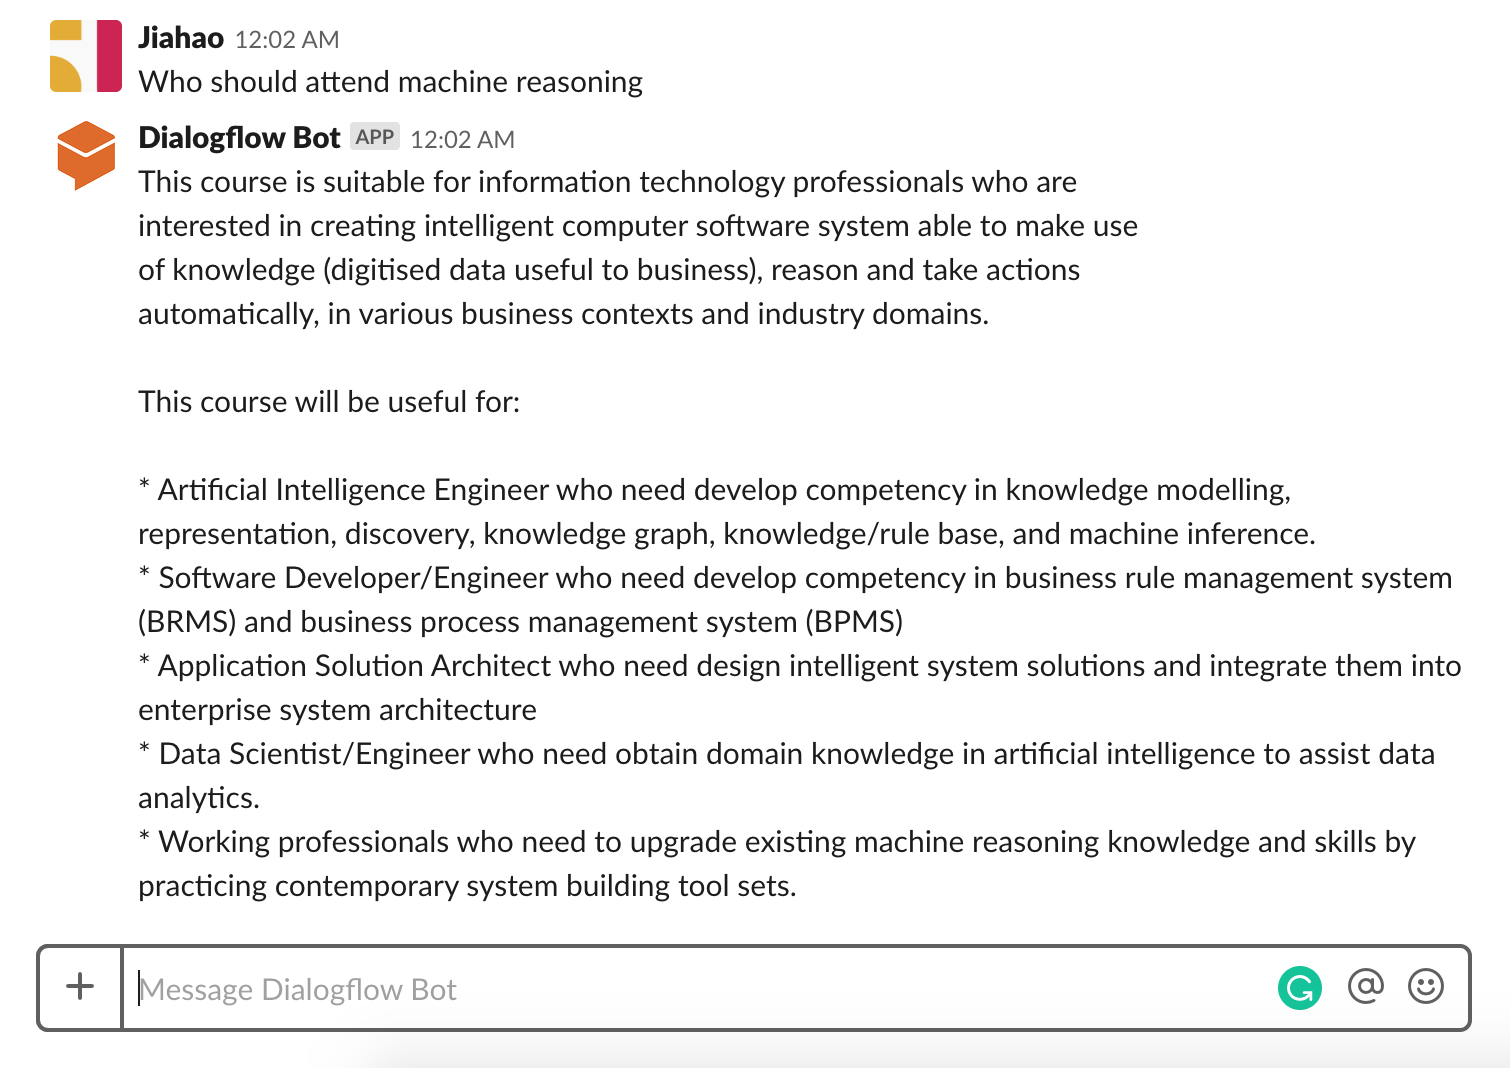
\includegraphics[width=\linewidth, frame]{img/scenario_2_3.png}
		\end{figure}

		\begin{figure}[H]
			\centering
			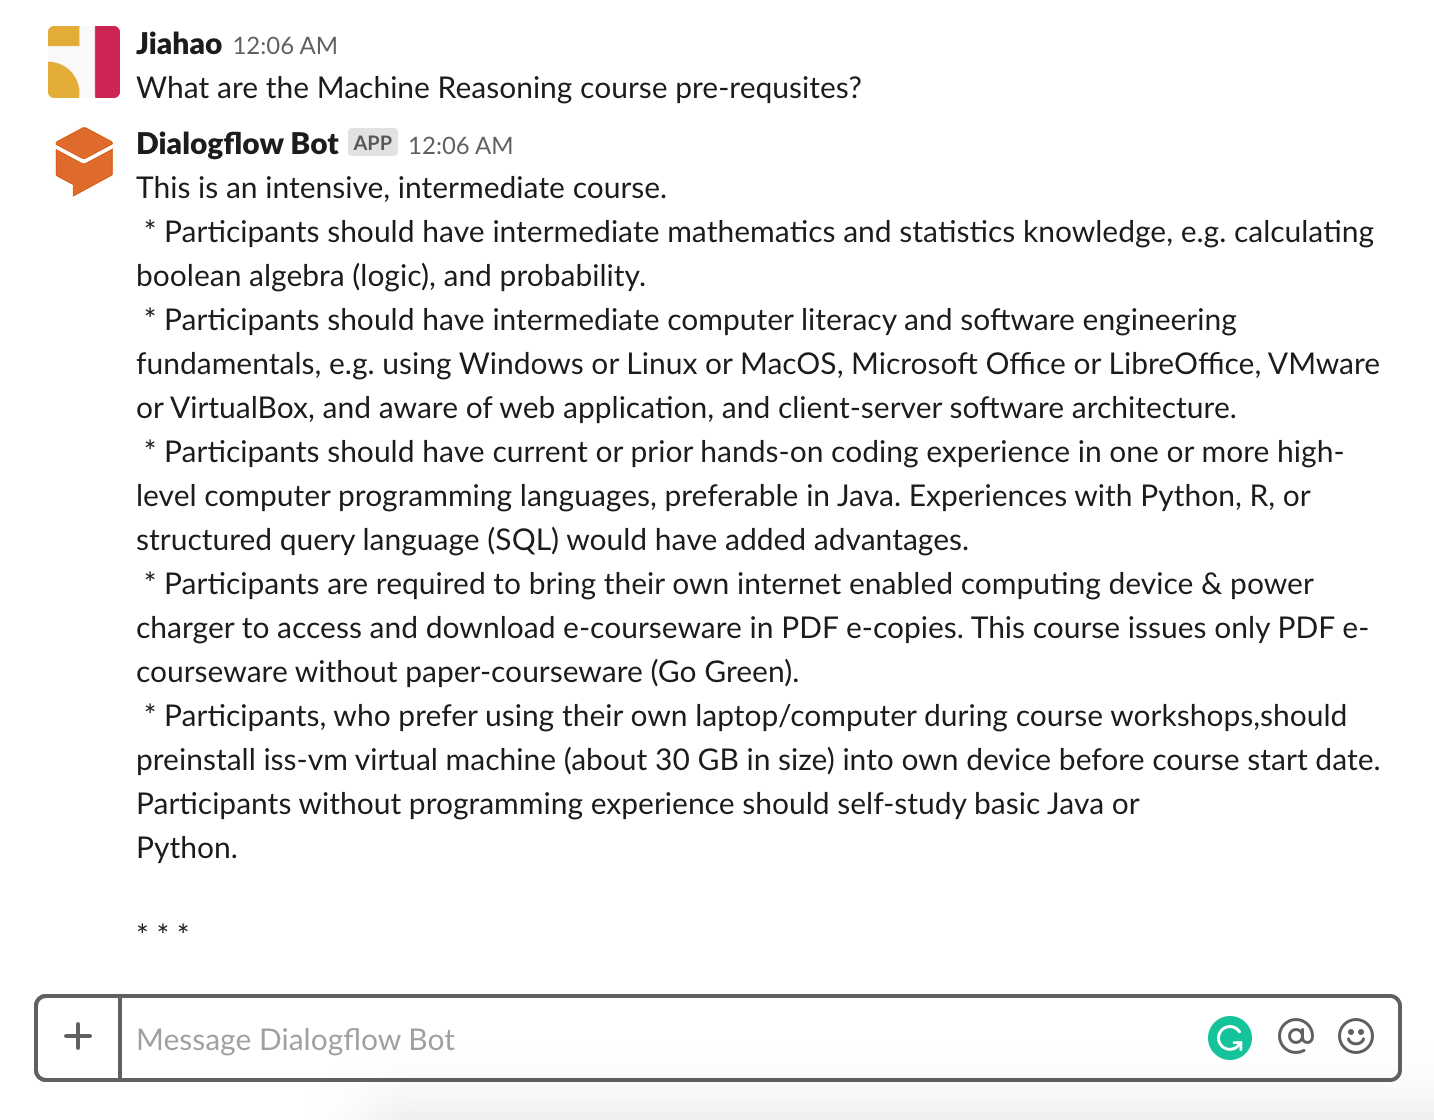
\includegraphics[width=\linewidth, frame]{img/scenario_2_4.png}
		\end{figure}
	% section scenario_2 (end)
% chapter demo (end)



\chapter{Project Related Files} % (fold)
\label{sub:project_related_files}
	\textbf{Presentation Video:} \url{https://youtu.be/QOxnEkNSttI}

	\textbf{Intent and Test:} \url{https://github.com/yaaazhiii/IRS-CS-2019-04-27-IS1PT-GRP-IChat/blob/master/Miscellaneous/Intent%20and%20Test.xlsx}

% section project_related_files (end)


% section appendices (end)